%%%%%%%%%%%%%%%%%%%%%%%%%%%%%%%%%%%%%%%%%%%%%%%%%%%
%
%  New template code for TAMU Theses and Dissertations starting Fall 2012.  
%  For more info about this template or the 
%  TAMU LaTeX User's Group, see http://www.howdy.me/.
%
%  Author: Wendy Lynn Turner 
%	 Version 1.0 
%  Last updated 8/5/2012
%
%%%%%%%%%%%%%%%%%%%%%%%%%%%%%%%%%%%%%%%%%%%%%%%%%%%
%%%%%%%%%%%%%%%%%%%%%%%%%%%%%%%%%%%%%%%%%%%%%%%%%%%%%%%%%%%%%%%%%%%%%%
%%                           SECTION III
%%%%%%%%%%%%%%%%%%%%%%%%%%%%%%%%%%%%%%%%%%%%%%%%%%%%%%%%%%%%%%%%%%%%%



\chapter{\uppercase{Grey Thermal Radiative Transfer- Numerical Results}}
\label{sec:chapter6_grey_radtran_results}


We now consider several test problems to verify and demonstrate the capability of the self-lumping DFEM spatial discretizations we have developed to solve the grey TRT equations.
First, in \secref{sec:chap6_analytic_results} we will consider problems with analytic solutions to verify and demonstrate the asymptotic convergence rates of our DFEM and SDIRK discretizations of the grey thermal radiative transfer equations.
In \secref{sec:marshak_waves}, we will consider two Marshak wave problems.  
A Marshak wave test problem consists of an initially cold slab that is heated by a strong, incident photon source, and is characteristic of several thermal radiative transfer problems of interest, such as inertial confinement fusion.
Finally, we summarize the effectiveness of the modified interior penalty diffusion synthetic acceleration operator in accelerating the iterative convergence of the grey TRT equations in \secref{sec:mip_results}.

We present numerical results for several DFEM schemes:
\begin{enumerate}
\item TL: traditional mass matrix lumping using equally-spaced interpolation points with cell-wise constant material properties,
\item SL Lobatto: self-lumping quadrature using Lobatto interpolation points with cell-wise constant material properties,
\item SL Gauss: self-lumping quadrature using Gauss interpolation points with cell-wise constant material properties, 
\item SLXS Lobatto: self-lumping quadrature using Lobatto interpolation points with approximate integration of spatially varying $\mathbf{R}$, and
\item SLXS Gauss: self-lumping quadrature using Gauss interpolation points with approximate integration of spatially varying $\mathbf{R}$.
\end{enumerate}  
In problems where opacities and heat capacities are constant functions of temperature, SL Lobatto is equivalent to SLXS Lobatto and SL Gauss is equivalent to SLXS Gauss.
However, for problems with temperature dependent material properties, SL Lobatto and SL Gauss will approximate the within cell variation of material properties assuming a cell-wise constant equal to the volumetric average of each material property, whereas SLXS Gauss and SLXS Lobatto will explicitly account for the within cell variation of material properties following the example of \eqt{eq:chap3_sl_react}.

Accuracy comparisons will be based upon the discrete $L_2$ norm of the error in angle integrated intensity, $E_{\phi} = \norm{ \widetilde{\phi}(x) - \phi(x)}_{L^2}$, and the $L_2$ error in temperature, $E_T = \norm{ \widetilde{T}(x) - T(x) }_{L^2}$.
We calculate $E_{\phi}$ as
\benum
E_{\phi} = \sqrt{\sum_{c=1}^{N_{cell}}{ \frac{\Delta x_c}{2} \sum_{q=1}^{N_{qf}}{ w_q \left(\widetilde{\phi}(s_q , t_{end}) - \phi(s_q,t_{end})  \right)^2 } } }\pec
\label{eq:e_phi_6}
\eenum
where $w_q$, $s_q$ are Gauss quadrature points and $N_{qf} = 2P+7$, and $P$ is the DFEM trial space degree.  
$E_{T}$ is calculated analogously to $E_{\phi}$.
Additionally, we will consider $L^2$ like norms of the cell average angle integrated intensity, $E_{\phi_A}$, and cell average temperature error, $E_{T_A}$.
$E_{\phi_A}$ is approximated as:
\benum
E_{\phi_A} = \sqrt{
\sum_{c=1}^{N_{cell}}{ 
\frac{\Delta x}{2} 
\left( 
\frac{1}{2}\sum_{q=1}^{N_{qf}}{ w_q \widetilde{\phi}(s_q , t_{end})}  - \frac{1}{2}\sum_{q=1}^{N_{qf}}{ w_q \phi(s_q , t_{end})} 
\right)^2 
} 
} \pec
\eenum
with $N_{qf}$ defined as in \eqt{eq:e_phi_6}.  $E_{T_A}$ is estimated in a similar fashion.

\section{Problems with Analytic Solutions}
\label{sec:chap6_analytic_results}

\subsection{Su-Olson Problem}

The Su-Olson problem \cite{su_olson_1} is an analytic benchmark that consists of an initially cold (initial radiation energy density and temperature conditions are identically absolute zero) half-space slab, heated for a finite amount of time by a volumetric, isotropic radiation source.
The slab's scattering and absorption opacities are constant in space and temperature and $C_v \propto T^3$.
Assuming $C_v = \alpha T^3$ is critical; as Long, et al. \cite{alex_paper} noted, the assumption regarding $C_v$ is not physical, but is required to make the thermal radiative transfer equations linear in $I$ and $T^4$, or conversely linear in $I$ and material energy density. 
After a series of transformations, Su and Olson derived an analytic solution to the thermal radiative transfer equations under these conditions; their solution is more accurately described as being semi-analytic.
While the radiation energy density and material temperature at every point can be expressed as a closed form integral, evaluation of each integral requires numerical estimation.
Further, the integral is a 2-D, indefinite integral (in both variables) of a trigonometric function with a slowly  decaying exponential argument.
However, \cite{su_olson_1} provides several radiation energy density and material energy density points in space, and thus the Su-Olson problem is beneficial as a benchmark problem to verify the physics of a given radiative transfer implementation.

Given the initial temperature condition is explicitly zero, this implies the initial $C_v$ is also zero.
This is problematic when solving explicitly for temperature and not material energy.
A near-zero heat capacity would result in the material rapidly heating, but a zero heat capacity implies a material that cannot accept heat, and thus can never be heated up.
To prevent this problem, we modify the definition of $C_v$:
\benum
C_v = 10^{-8} + \alpha T^3 \pep
\eenum
Alternatively, we could set an initial temperature to be a non absolute zero value.

Since \cite{su_olson_1} presents results in a non-dimensional format, we elect to define $a=c=1$, $\sigma_a = 1$, $\sigma_s=0$, $\alpha = 4$, truncate the full half space to $x\in[0,5]$, and define the reference temperature, $T_H = 1$.
We solve the problem using 200 spatial mesh cells, linear SLXS Lobatto, the SDIRK 2-2 time differencing scheme, an initial time step size of $\Delta t = 10^{-5}$, and increase the time step size by a factor of 1.1 until a maximum time step size of $\Delta t = 10^{-3}$ is reached.

In \fig{fig:su_olson_s2_rad} we present the radiation energy density solution, ($W(x)$ in the notation on \cite{su_olson_1}) for $S_2$ angular differencing plotted against the analytic diffusion and transport solutions.  Likewise, in \fig{fig:su_olson_s2_mat}, we plot the material energy density ($V(x)$ in the notation on \cite{su_olson_1}) for $S_2$ angular differencing.
Solutions at non-dimensional times $\tau = 1$ and $\tau=10$ are given in both plots.
As expected, the $S_2$ solution is nearly identical to diffusion, but skews slightly in the direction of the full transport solution.
\begin{figure}[!htp]
\centering
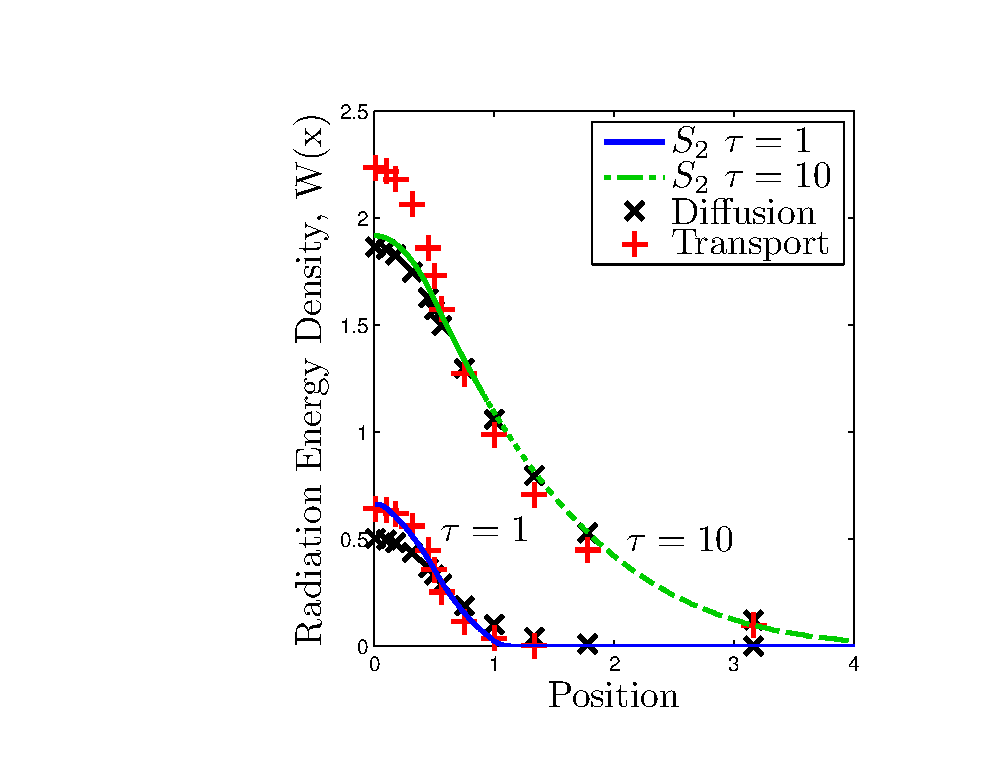
\includegraphics[width=8cm,trim=1.75in  0.5in 0.75in 0.5in,clip=true]{chapter6_grey_radtran/Dissertation_Data/Su_Olson_S2_Radiation_Energy.pdf}
\caption{$S_2$ radiation energy density profile for Su-Olson problem.}
\label{fig:su_olson_s2_rad}
\end{figure}
\begin{figure}[!hbp]
\centering
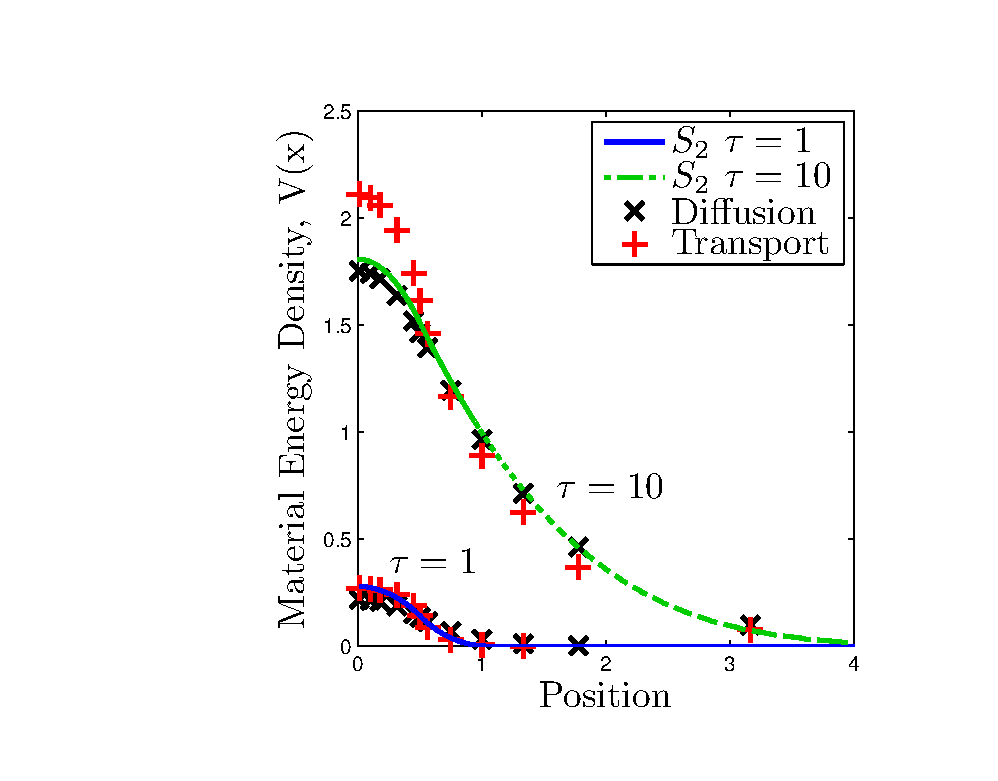
\includegraphics[width=8cm,trim=1.75in  0.5in 0.75in 0.5in,clip=true]{chapter6_grey_radtran/Dissertation_Data/Su_Olson_S2_Material_Energy.pdf}
\caption{$S_2$ material energy density profile for Su-Olson problem.}
\label{fig:su_olson_s2_mat}
\end{figure}

Increasing the number of discrete ordinates, the radiation energy density profile and material energy density profiles are given in \fig{fig:su_olson_s8_rad} and \fig{fig:su_olson_s8_mat} for $S_8$ angular differencing.
\begin{figure}[!htp]
\centering
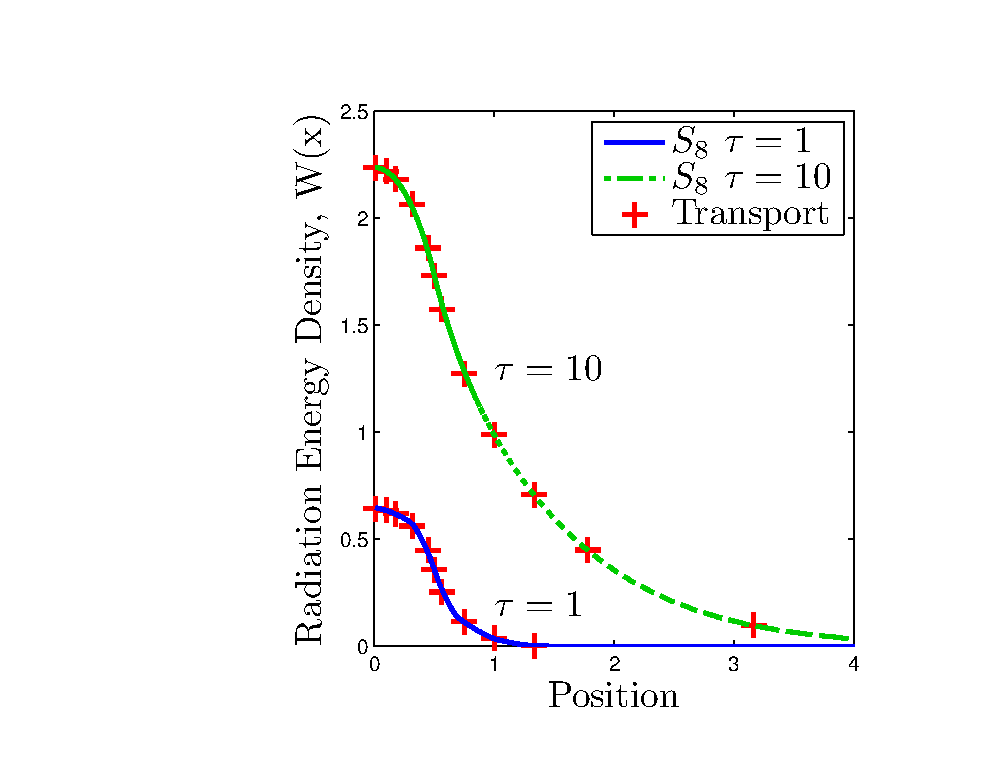
\includegraphics[width=8cm,trim=1.75in  0.5in 0.75in 0.5in,clip=true]{chapter6_grey_radtran/Dissertation_Data/Su_Olson_S8_Radiation_Energy.pdf}
\caption{$S_8$ radiation energy density profile for Su-Olson problem.}
\label{fig:su_olson_s8_rad}
\end{figure}
\begin{figure}[!htp]
\centering
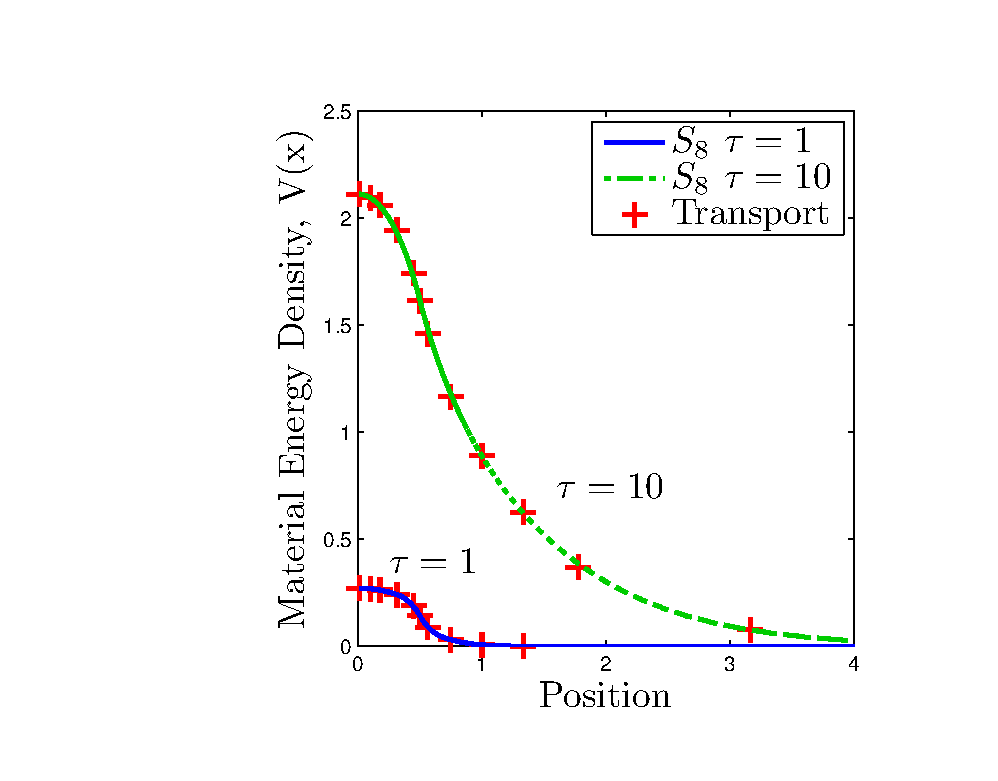
\includegraphics[width=8cm,trim=1.75in  0.5in 0.75in 0.5in,clip=true]{chapter6_grey_radtran/Dissertation_Data/Su_Olson_S8_Material_Energy.pdf}
\caption{$S_8$ material energy density profile for Su-Olson problem.}
\label{fig:su_olson_s8_mat}
\end{figure}
By adding a few discrete directions to the quadrature set, our numerical solution becomes indistinguishable from published results of \cite{su_olson_1}, and we conclude that our TRT equation implementation is valid.

\newpage

\subsection{Method of Manufactured Solutions}

The method of manufactured solutions, MMS, consists of choosing an analytic solution, then defining the driving source necessary to achieve that solution \cite{mms}.
Though MMS solutions are derived, they are excellent for testing the convergence of numerical methods devised to solve complex physics phenomena.
While analytic solutions that do not use exotic source terms are more appealing for verification purposes, these types of solutions are difficult to devise for complex physics phenomena, especially for coupled physical phenomena like radiative transfer.  
For those multiphysics problems for which an analytic solution does exist, the solutions are usually semi-analytic, and cannot be used effectively as a reference solution for a convergence study because the semi-analytic solution has numerical errors of the same magnitude (or greater) than the numerical simulations we are attempting to verify.
%Similarly experimental results will contain measurement errors, and will almost certainly be of low resolution, either measuring only integral quantities, or providing data at only a few points in space, and thus do not permit convergence studies.

We elect to choose separable manufactured solutions of the form:
\begin{subequations}
\beanum
I_d(x,\mu_d,t) &=& M(\mu_d) F(t) W_I(x) \\
T(x) &=& F(t) W_T(x) \\
\phi(x) &=& C_M F(t) W_I(x) \\
C_M &=& \sum_{d=1}^{N_{dir}} { w_d M(\mu_d) } \pep
\eeanum
\label{eq:mms_solns}
\end{subequations}
where $M(\mu_d)$ is as angular component of the intensity solution desired, $I_d(x,\mu_d,t)$; $F(t)$ is the time component of the manufactured solution, chosen to be the same for the angular intensity, angle integrated intensity, and temperature; $W_I(x)$ is the spatial component of the angular intensity; and $W_T(x)$ is the spatial component of the temperature solutions.
The definition of $C_M$ given in \eqts{eq:mms_solns} and $W_I(x)$ being the spatial component of $\phi$ is required for the $S_N$ approximation to be true.

For all MMS simulations, our initial conditions are
\beanum
I(x,\mu_d,t_0) &=& M(\mu_d)W_I(x)F(t_0) \\
T(x,t_0) &=& W_T(x)F(t_0) \\
\phi(x,t_0) &=& \left[ \sum_{d=1}^{N_{dir}}{w_d M(\mu_d)} \right] W_I(x)F(t_0) \pep
\eeanum
Likewise, we always use an incident flux intensity boundary condition, for $\mu_d >0$:
\benum
I_{in}(\mu_d,t) = M(\mu_d) W_I(x_{1/2}) F(t) \pec
\eenum
and for $\mu_d < 0$
\benum
I_{in}(\mu_d,t) = M(\mu_d) W_I(x_{N_{cell}+1/2}) F(t) \pec
\eenum
where $x_{1/2}$ is the left domain boundary and $x_{N_{cell}+1/2}$ is the right domain boundary.
We do not impose, and no boundary conditions are required for the material temperature.
We evaluate $\vec{S}_I$ and $\vec{S}_T$ using the spatially analytic definitions of $S_I$ and $S_T$ respectively, and numerically integrate the source moments using a $N_q$ Gauss-Legendre quadrature points, with $N_q = 2N_P + 5$, and $N_P$ is the number of DFEM interpolation points, as defined previously.

\subsubsection{Linear in Time - Trigonometric in Space  }
In our first method of manufactured solutions problem, MMS1, we design a source whose radiation and temperature solutions is a cosine in space and  linear in time.
We use a non-dimensional form of the TRT, assume that $a=c=1$, and that material opacities and heat capacities are constant functions of space and temperature.
We impose the solution:
\beanum
M(\mu_d) &=& \frac{1}{4\pi} \\
W_I(x) &=& 10 \cos\left( \frac{\pi x}{10} - \frac{\pi}{2} \right) + 15\\
W_T(x) &=&  25 \cos\left( \frac{\pi x}{10} - \frac{\pi}{2} \right) + 30\\
F(t) &=& 1+.02t \pep
\eeanum
Physically, $x\in[0,10]$, $C_v = 0.1$, $\sigma_a = 100.0$, $\sigma_s = 0.5$, we start the simulation at $t_0 = 0$, end the simulation at $t_{end}=1$, 
taking 100 equal time steps of length $\Delta t = 0.01$, with the SDIRK 2-2 scheme.  

Figure \ref{fig:mms1_tl_phi}, \fig{fig:mms1_lobatto_phi}, and \fig{fig:mms1_gauss_phi} plot the order of convergence of $E_{\phi}$ for the TL, SL Lobatto, and SL Gauss schemes, respectively, as a function of trial space degree and cell size.
Analogous data for $E_{T}$ is given in \figs{fig:mms1_tl_temp}{fig:mms1_gauss_temp}.
%
\begin{figure}[!htp]
\centering
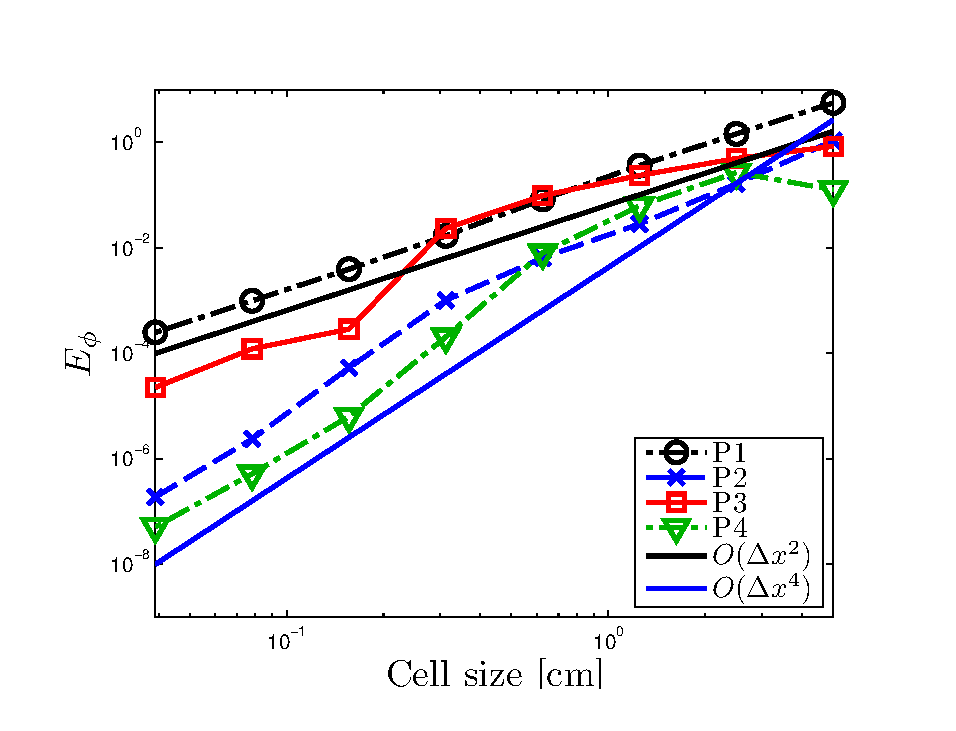
\includegraphics[width=10cm,trim=0.25in  0.5in 0.75in 0.75in,clip=true]{chapter6_grey_radtran/Dissertation_Data/MMS2_TL_phi_L2.pdf}
\caption{Convergence of $E_{\phi}$ for the TL scheme in problem MMS1.}
\label{fig:mms1_tl_phi}
\end{figure}
%
%
\begin{figure}[!hbp]
\centering
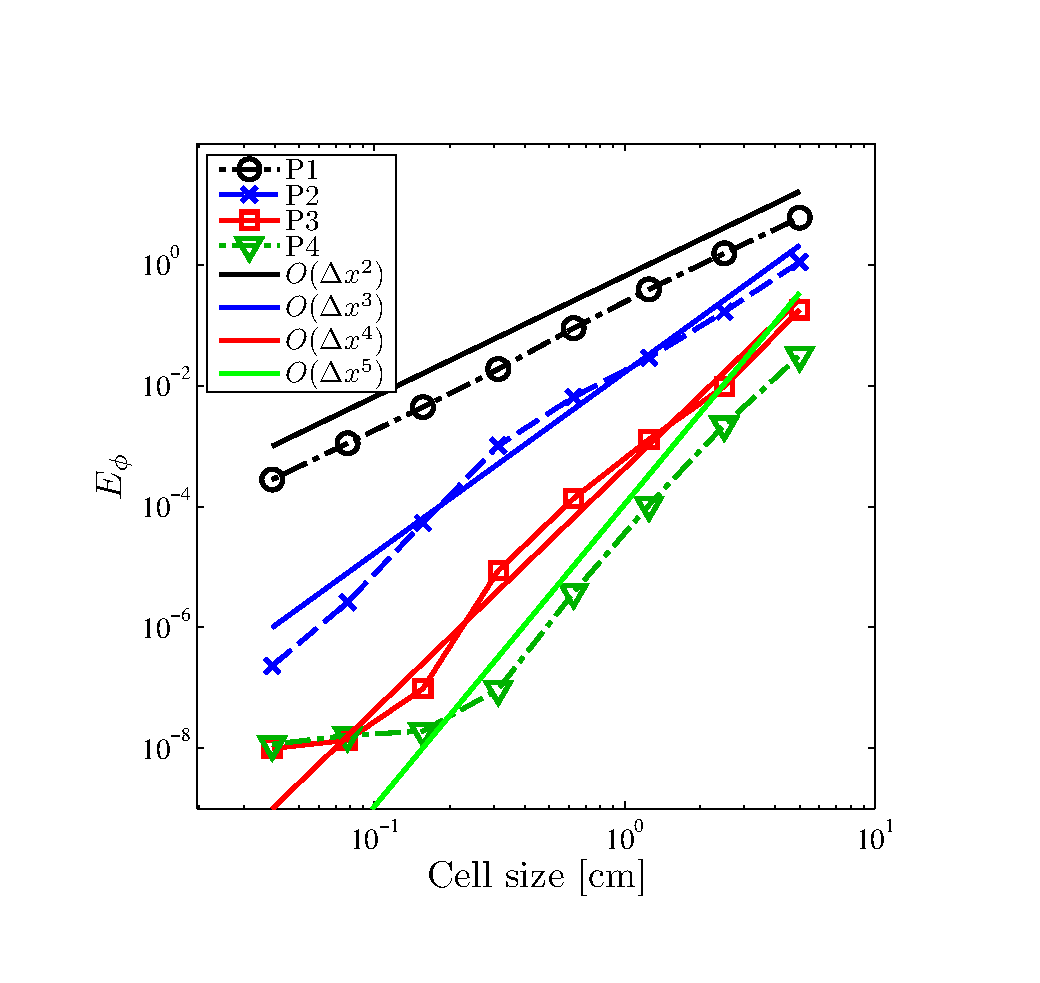
\includegraphics[width=10cm,trim=0.25in  0.5in 0.75in 0.75in,clip=true]{chapter6_grey_radtran/Dissertation_Data/MMS2_SLXS_Lobatto_phi_L2.pdf}
\caption{Convergence of $E_{\phi}$ for the SL Lobatto scheme in problem MMS1.}
\label{fig:mms1_lobatto_phi}
\end{figure}
%
%
\begin{figure}[!htp]
\centering
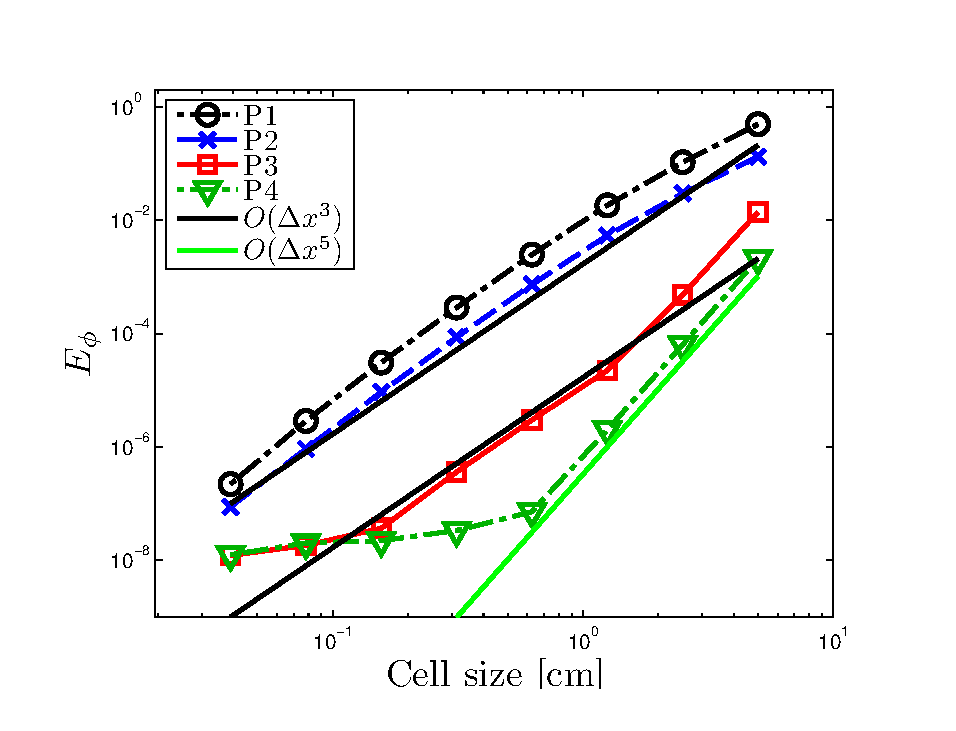
\includegraphics[width=10cm,trim=0.25in  0.5in 0.75in 0.75in,clip=true]{chapter6_grey_radtran/Dissertation_Data/MMS2_SLXS_Gauss_phi_L2.pdf}
\caption{Convergence of $E_{\phi}$ for the SL Gauss scheme in problem MMS1.}
\label{fig:mms1_gauss_phi}
\end{figure}
%
\begin{figure}[!hbp]
\centering
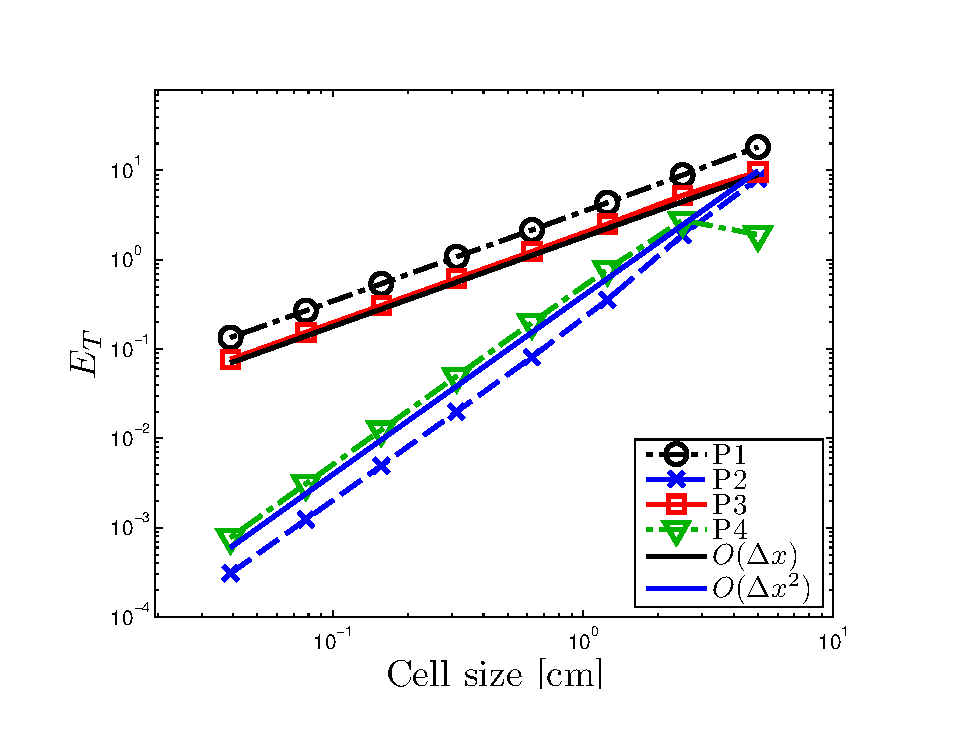
\includegraphics[width=10cm,trim=0.25in  0.5in 0.75in 0.75in,clip=true]{chapter6_grey_radtran/Dissertation_Data/MMS2_TL_temp_L2.pdf}
\caption{Convergence of $E_{T}$ for the TL scheme in problem MMS1.}
\label{fig:mms1_tl_temp}
\end{figure}
%
%
\begin{figure}[!htp]
\centering
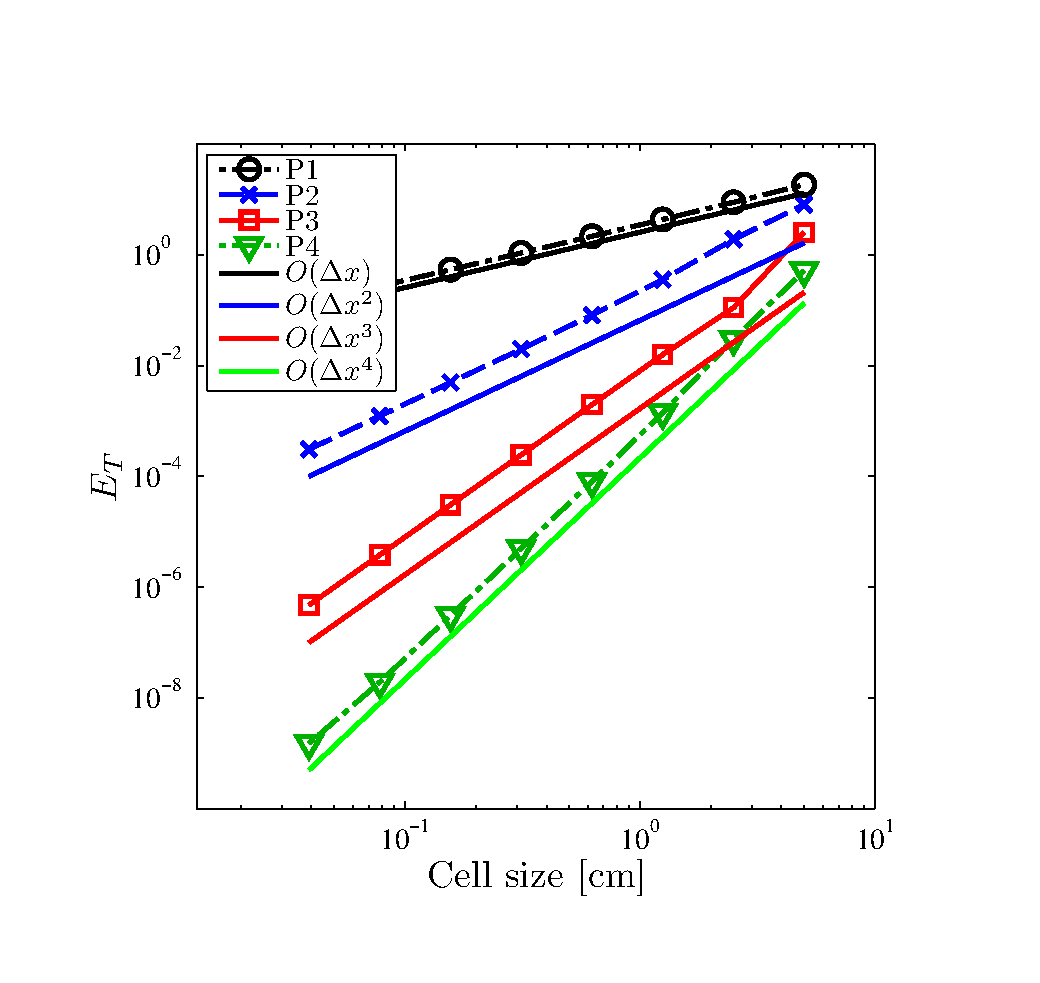
\includegraphics[width=10cm,trim=0.25in  0.5in 0.75in 0.75in,clip=true]{chapter6_grey_radtran/Dissertation_Data/MMS2_SLXS_Lobatto_temp_L2.pdf}
\caption{Convergence of $E_{T}$ for the SL Lobatto scheme in problem MMS1.}
\label{fig:mms1_lobatto_temp}
\end{figure}
%
%
\begin{figure}[!hbp]
\centering
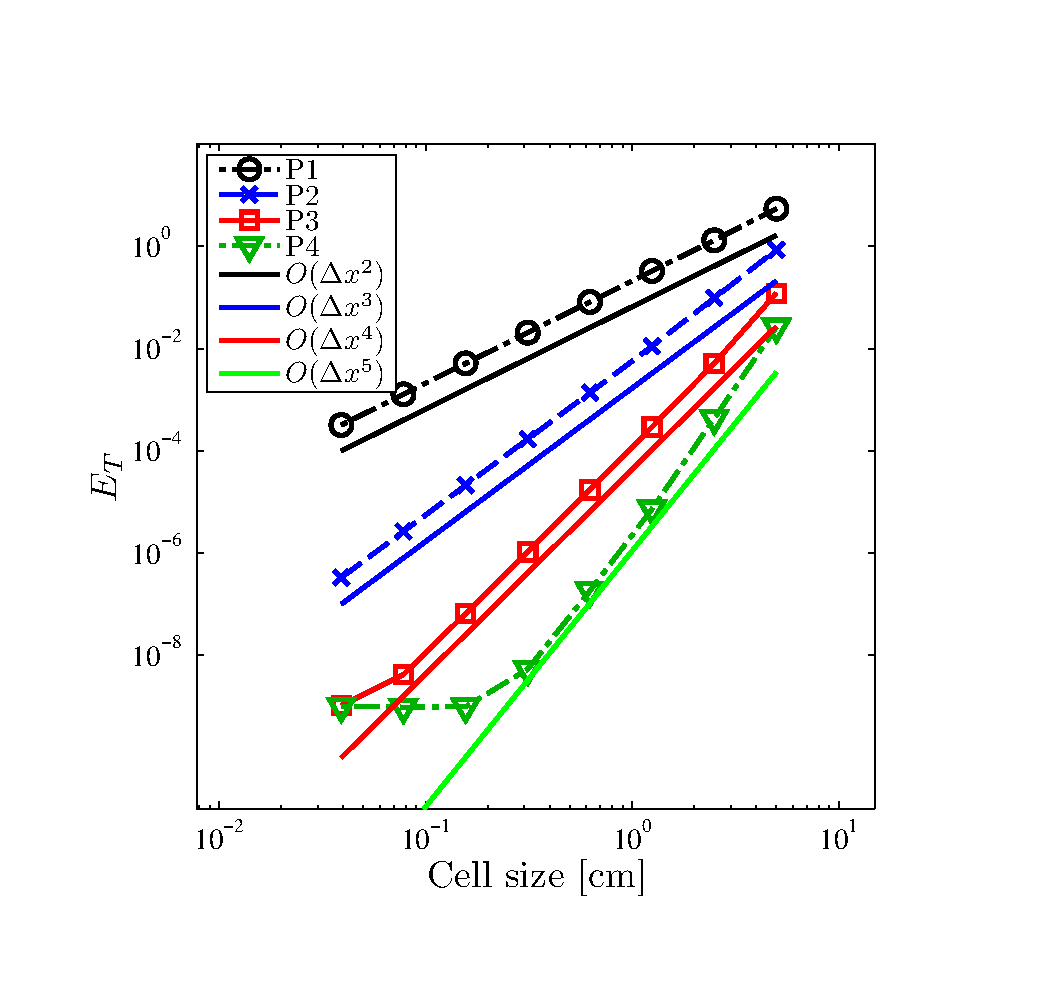
\includegraphics[width=10cm,trim=0.25in  0.5in 0.75in 0.75in,clip=true]{chapter6_grey_radtran/Dissertation_Data/MMS2_SLXS_Gauss_temp_L2.pdf}
\caption{Convergence of $E_{T}$ for the SL Gauss scheme in problem MMS1.}
\label{fig:mms1_gauss_temp}
\end{figure}

We make several observations regarding \figs{fig:mms1_tl_phi}{fig:mms1_gauss_temp}.  
First, the TL scheme does not necessarily increase in accuracy with an increase in trial space degree.
TL convergence of $E_{\phi}$ is limited to second order in space for odd degree trial space DFEM and third order spatial convergence for even degree trial space schemes, behavior identical to that demonstrated in our neutron transport testing.
A similar limit exists for TL convergence of $E_T$; TL converges $E_T$ at most first order for odd trial space DFEM and second order for even trial space degree DFEM.
Second, SL Lobatto converges the $L^2$ norm of the angle integrated intensity $\propto P+1$, the same order of convergence achieved in our neutron transport test problems for the convergence of $L^2$ error of the angular and scalar fluxes.
However, SL Lobatto only converges $E_T \propto P$, not $P+1$, as was the case for the neutron transport interaction rate.
Finally, SL Gauss converges $E_{\phi}$ and $E_T$ $\propto P+1$, the same order of convergence as seen with neutron transport.

Convergence of $E_{\phi_A}$ is given in \fig{fig:mms1_lobatto_phi_A} for SL Lobatto and \fig{fig:mms1_gauss_phi_A} for SL Gauss.
Convergence of $E_{T_A}$ is given in \figs{fig:mms1_lobatto_temp_A}{fig:mms1_gauss_temp_A} for SL Lobatto and SL Gauss, respectively.
No definitive pattern emerges in the convergence of $E_{\phi_A}$ as a function of $P$ for SL Lobatto in \fig{fig:mms1_lobatto_phi_A} when considering linear through quartic polynomial trial spaces, though SL Lobatto convergence of $E_{\phi_A}$ looks to be $\propto 2P$ or slightly less.
SL Lobatto's apparent order of convergence for $E_{\phi_A}$ for TRT problems as shown in \fig{fig:mms1_lobatto_phi_A} is less than SL Lobatto convergence of $E_{\psi_A}$ for neutron transport (\figs{fig:multi_L2A_p1}{fig:multi_L2A_p4}), but not significantly. 
Similarly, the radiative transfer variant of SL Gauss does not converge $E_{\phi_A}$ for TRT simulations consistently $\propto 2P+1$ as SL Gauss converged $E_{\psi_A}$ neutron transport problems,
but it is close.  
Interestingly, the observed decreases in the convergence of $E_{\phi_A}$ for SL Lobatto and SL Gauss when applied to TRT relative to neutron transport convergence of $E_{\psi_A}$ does not hold when considering the convergence of $E_{T_A}$.  
SL Lobatto converges $E_{T_A}$ for TRT with the same order as SL Lobatto converges $E_{\psi_A}$ and $E_{IR_A}$ for neutron transport, $\propto 2P$.
SL Gauss actually exhibits an $E_{T_A}$ order of convergence that appears to exceed its neutron transport analog, converging $E_{T_A} \propto 2P+2$. \

\begin{figure}[!htp]
\centering
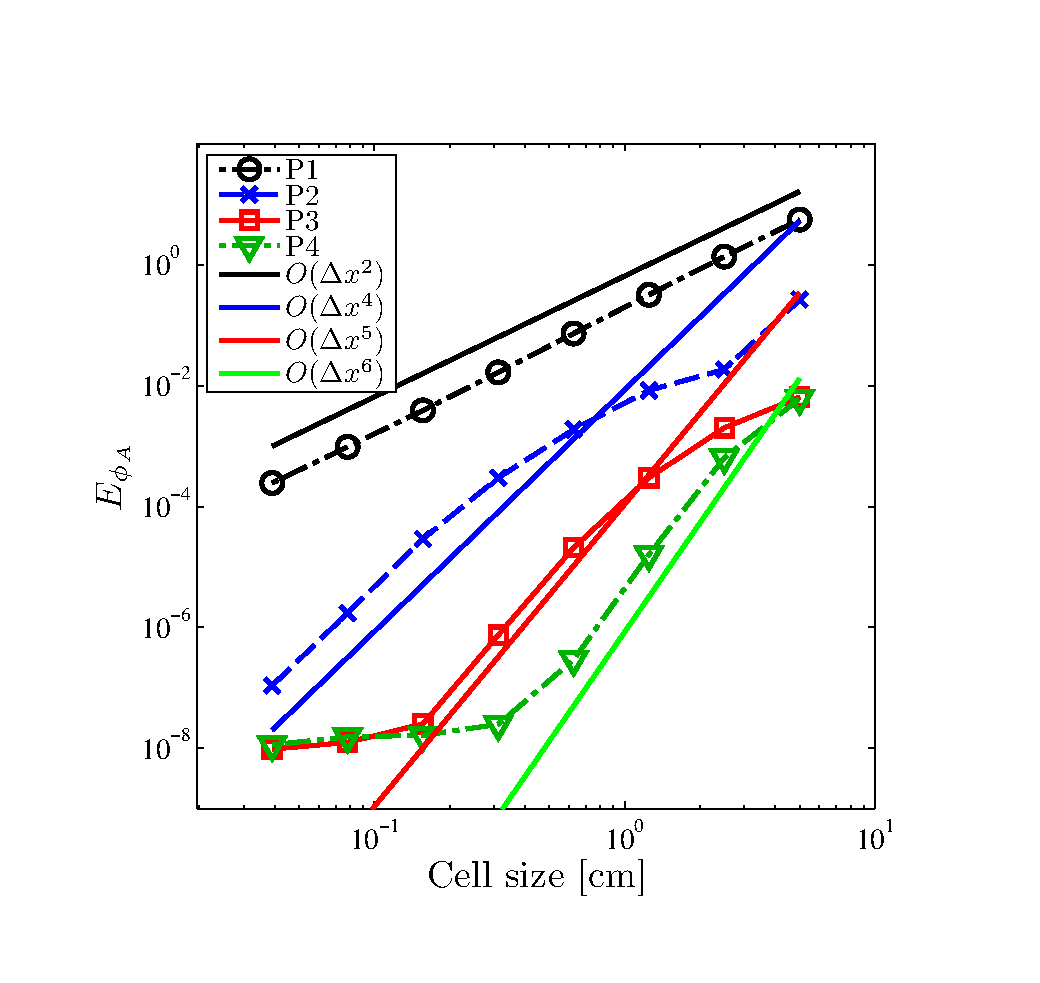
\includegraphics[width=9cm,trim=0.25in  0.5in 0.75in 0.75in,clip=true]{chapter6_grey_radtran/Dissertation_Data/MMS2_SLXS_Lobatto_phi_A.pdf}
\caption{Convergence of $E_{\phi_A}$ for the SL Lobatto scheme in problem MMS1.}
\label{fig:mms1_lobatto_phi_A}
\end{figure}
%
%
\begin{figure}[!hbp]
\centering
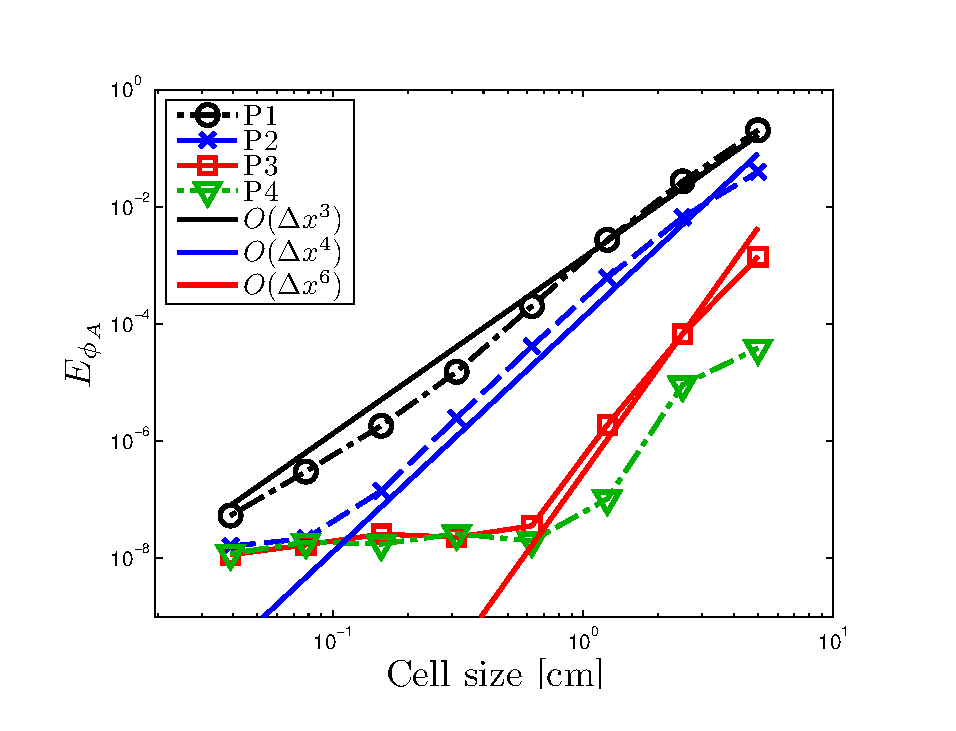
\includegraphics[width=9cm,trim=0.25in  0.1in 0.75in 0.5in,clip=true]{chapter6_grey_radtran/Dissertation_Data/MMS2_SLXS_Gauss_phi_A.pdf}
\caption{Convergence of $E_{\phi_A}$ for the SL Gauss scheme in problem MMS1.}
\label{fig:mms1_gauss_phi_A}
\end{figure}
%
%
\begin{figure}[!htp]
\centering
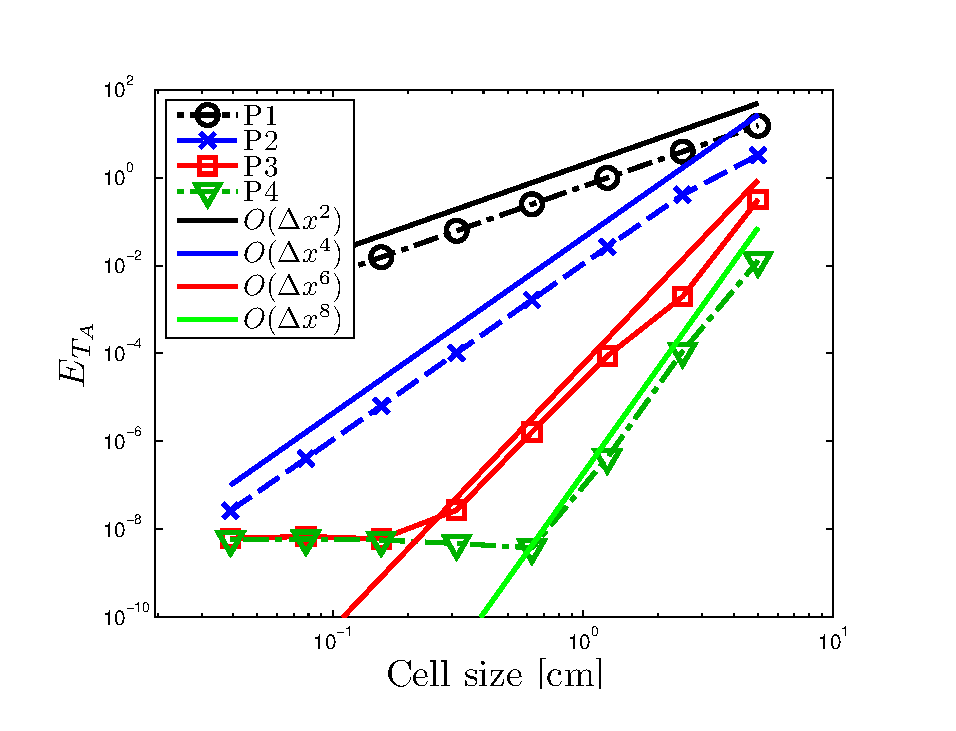
\includegraphics[width=10cm,trim=0.25in  0.5in 0.75in 0.75in,clip=true]{chapter6_grey_radtran/Dissertation_Data/MMS2_SLXS_Lobatto_temp_A.pdf}
\caption{Convergence of $E_{T_A}$ for the SL Lobatto scheme in problem MMS1.}
\label{fig:mms1_lobatto_temp_A}
\end{figure}
%
%
\begin{figure}[!hbp]
\centering
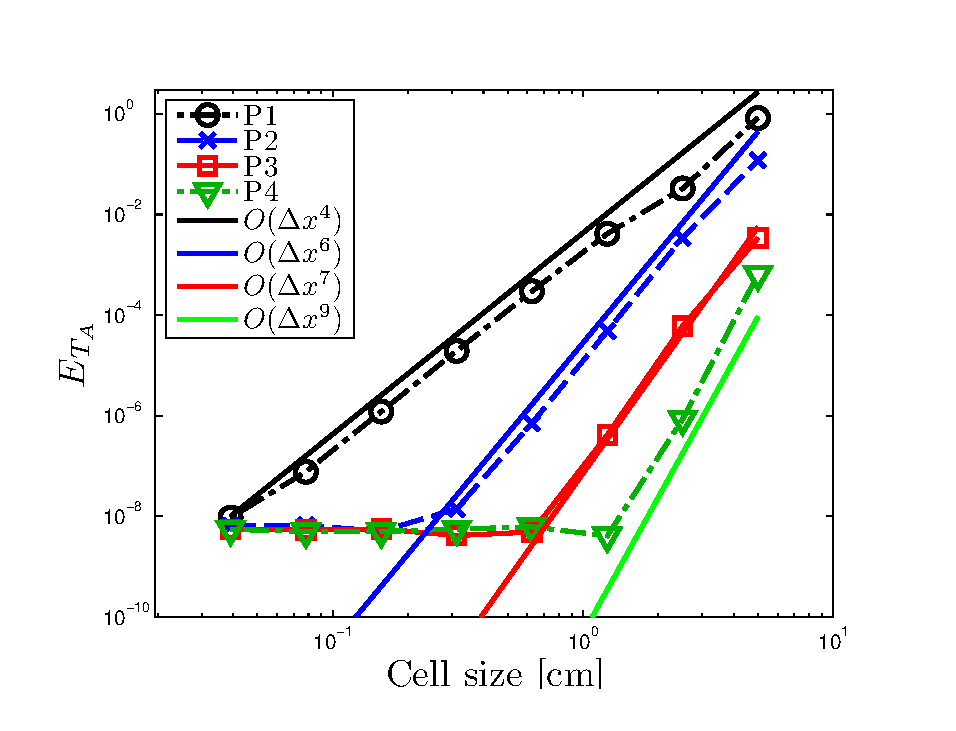
\includegraphics[width=10cm,trim=0.25in  0.5in 0.75in 0.75in,clip=true]{chapter6_grey_radtran/Dissertation_Data/MMS2_SLXS_Gauss_temp_A.pdf}
\caption{Convergence of $E_{T_A}$ for the SL Gauss scheme in problem MMS1.}
\label{fig:mms1_gauss_temp_A}
\end{figure}

It is our hypothesis that the apparent super convergence demonstrated by SL Gauss in converging $E_T$ is related to how we expand the Planckian in the same trial space as the DFEM temperature and radiation solutions. 
That is to say that we suspect the $N_P$ quadrature points of a given trial space degree SL Gauss scheme are significantly more accurate at integrating 
\benum
\B{i}(s) B(\widetilde{T}) \pec
\label{eq:planck_int}
\eenum
a degree $5P$ polynomial, than an $N_P$ Lobatto quadrature.
Though the $N_P$ point Gauss quadrature only exactly integrates polynomials of degree $2P+1$, it may be that the remaining terms are coincidentally very small in magnitude for a degree $5P$ polynomial of the particular nature of \eqt{eq:planck_int}.

%This plateauing of errors seen in the above plots is a result of two things.  
%First, the nested nature of our TRT solution algorithm.
%Due to the nested iterations, we must use the tightest tolerance on the innermost solve, the intensity update.
%We terminate the innermost solve after reaching a certain point-wise change tolerance, $\epsilon_{inner}$, of the zero-th angular moment of the angle integrated intensity: 
%\benum
%\max_{j} { \abs{ \frac{\phi_{j}^{(\ell+1)} - \phi_j^{(\ell)} }{\phi_{j}^{(\ell+1)} } }  } < \epsilon_{inner} \pep
%\eenum
%Similarly, the thermal iteration of SDIRK stage $s$ is terminated when every temperature solution at the DFEM interpolation points, $T_j$,  changes less than $\epsilon_{thermal}$,
%\benum
 %\max_{j} { { \abs{ \frac{ T_{j,s}^{(\ell+1)} - T_j^{(\ell)} }{T_{j}^{(\ell+1)} } }  } }< \epsilon_{thermal} \pep
%\eenum
%For this and all other MMS problems, $\epsilon_{inner} = 10^{-12}$ and $\epsilon_{thermal} = 10^{-10}$.
%Secondly, as the TRT equations are functions of space and time, it possible that the error of a given spatial discretization is smaller than the temporal error of the problem, thus a plateauing of the solution error as a function of spatial mesh refinement occurs.
%Thus, truly accurate solutions require the refinement of both spatial mesh and time step size.

\subsubsection{Trigonometric in  Space - Linear in Time - with Temperature Dependent Material Properties}

We now consider a problem with temperature dependent material properties, MMS2.  We impose the following solution:
\beanum
M(\mu_d) &=& \frac{1}{4\pi} \\
W_I(x) &=& 9 \cos\left( \frac{\pi x}{10} - \frac{\pi}{2} \right) + 3 \pec \\
W_T(x) &=&  5 \cos\left( \frac{\pi x}{10} - \frac{\pi}{2} \right) + 5 \pec \\
F(t) &=&  1 + .02t \pec
\eeanum
and define the following material properties:
\beanum
C_v &=& 0.2 + 0.01 T^3 \\
\sigma_a &=& \frac{10^4}{T^3} \\
\sigma_s &=& 0.5 \pep
\eeanum
In our problem, $x\in[0,10]$, $t\in[0,2]$ and we discretize in time using the SDIRK 3-3 scheme with $\Delta t = 0.001$.  
In total , we consider four different DFEM schemes for this problem, SL Lobatto, SL Gauss, SLXS Lobatto, and SLXS Gauss.  
To reiterate, methods denoted SL assume cell-wise constant opacities and heat capacities,  equal to the cell-wise volumetric average of that quantity;  
SLXS schemes explicitly account for the within cell variation of temperature dependent material properties by evaluating $\mathbf{R}$ as in \eqt{eq:chap3_sl_react}.
$E_{\phi}$ convergence for the SL Lobatto and SL Gauss schemes is plotted in \fig{fig:mms3_constant_lobatto_phi} and \fig{fig:mms3_constant_gauss_phi}, respectively.
\begin{figure}[!hbp]
\centering
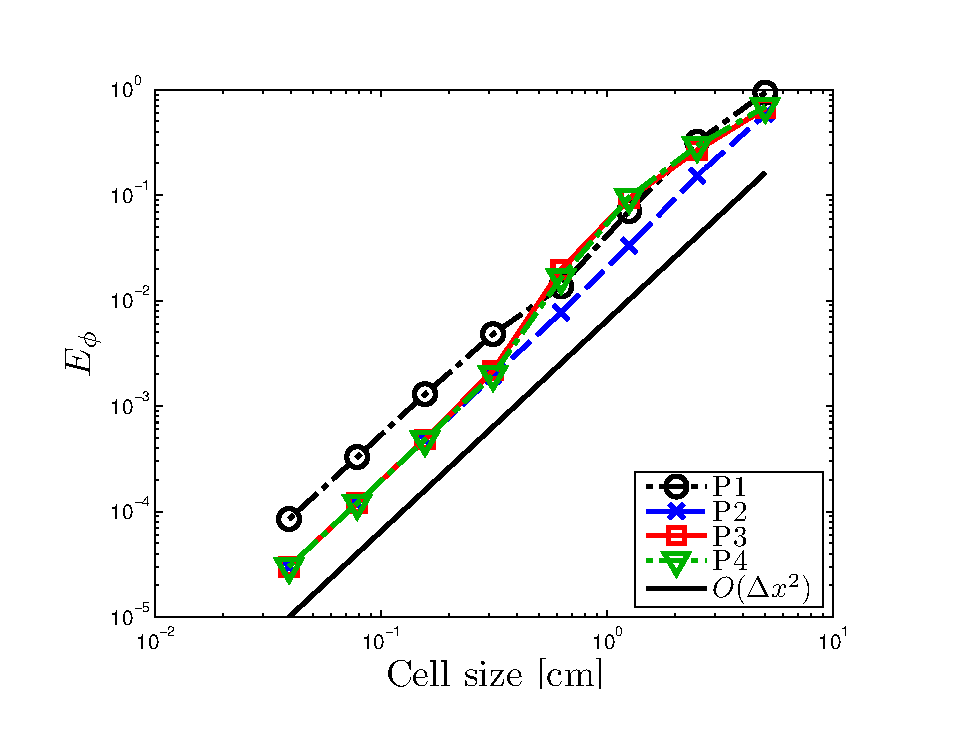
\includegraphics[width=10cm,trim=0.25in  0.25in 0.75in 0.5in,clip=true]{chapter6_grey_radtran/Dissertation_Data/MMS3_Constant_XS_SL_Lobatto_phi_L2.pdf}
\caption{Convergence of $E_{\phi}$ for the SL Lobatto scheme in problem MMS2.}
\label{fig:mms3_constant_lobatto_phi}
\end{figure}
%
%
\begin{figure}[!htp]
\centering
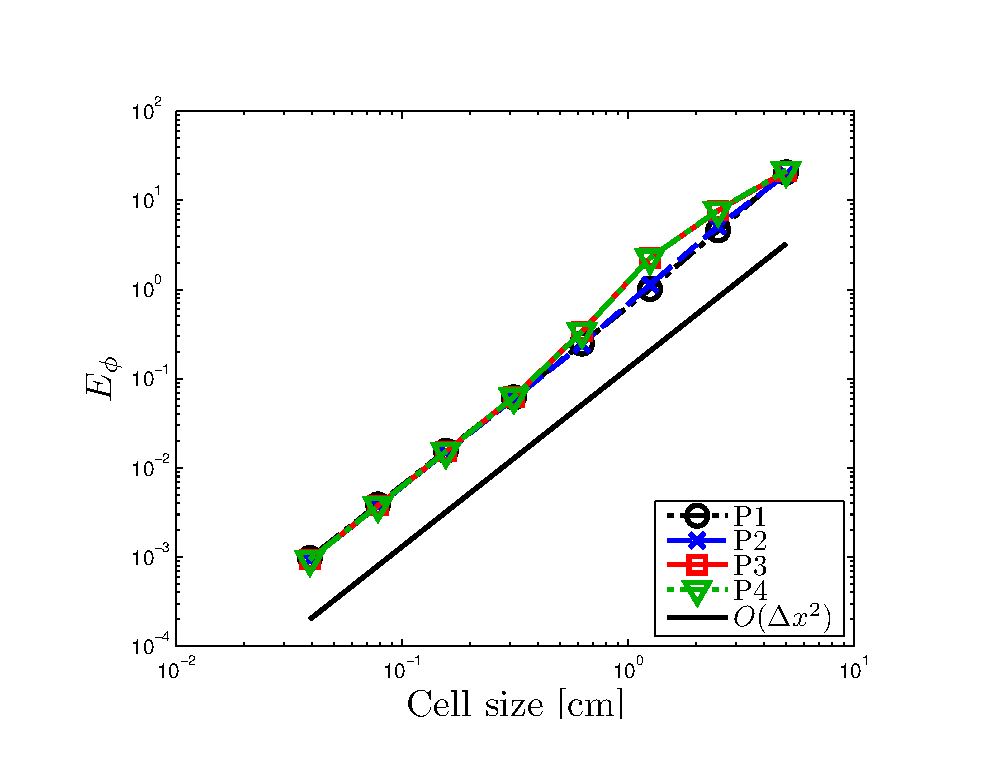
\includegraphics[width=10cm,trim=0.25in  0.25in 0.75in 0.5in,clip=true]{chapter6_grey_radtran/Dissertation_Data/MMS3_Constant_XS_SL_Gauss_phi_L2.pdf}
\caption{Convergence of $E_{\phi}$ for the SL Gauss scheme in problem MMS2.}
\label{fig:mms3_constant_gauss_phi}
\end{figure}
\begin{figure}[!hbp]
\centering
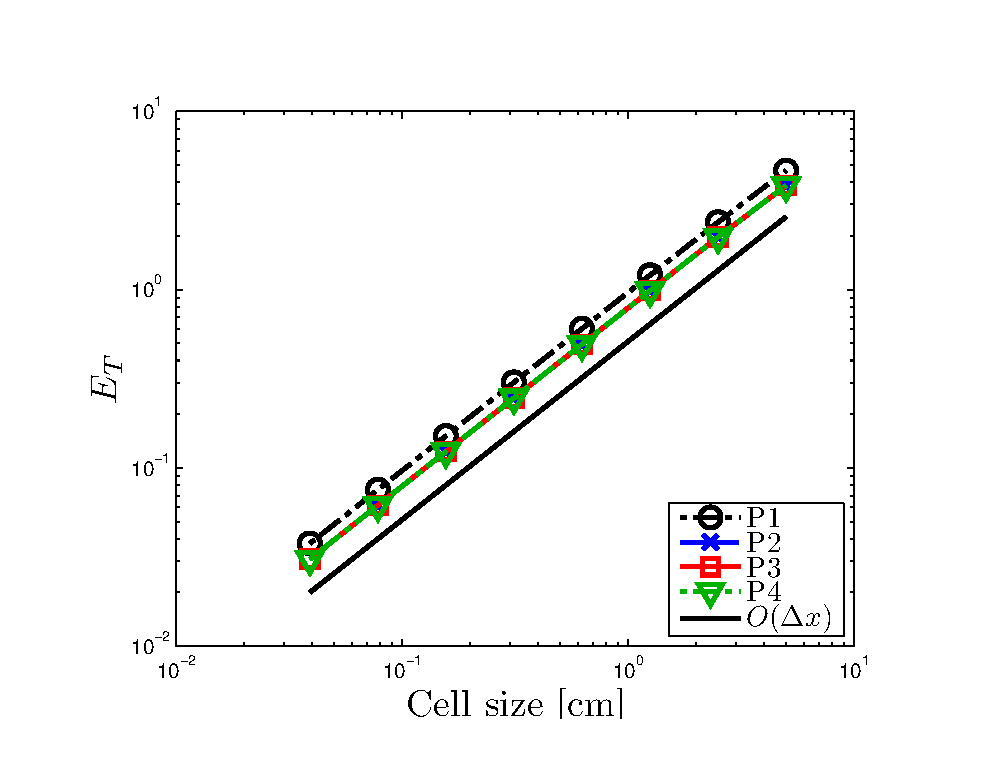
\includegraphics[width=10cm,trim=0.25in  0.2in 0.75in 0.5in,clip=true]{chapter6_grey_radtran/Dissertation_Data/MMS3_Constant_XS_SL_Lobatto_temp_L2.pdf}
\caption{Convergence of $E_{T}$ for the SL Lobatto scheme in problem MMS2.}
\label{fig:mms3_constant_lobatto_temp}
\end{figure}
%
%
\begin{figure}[!htp]
\centering
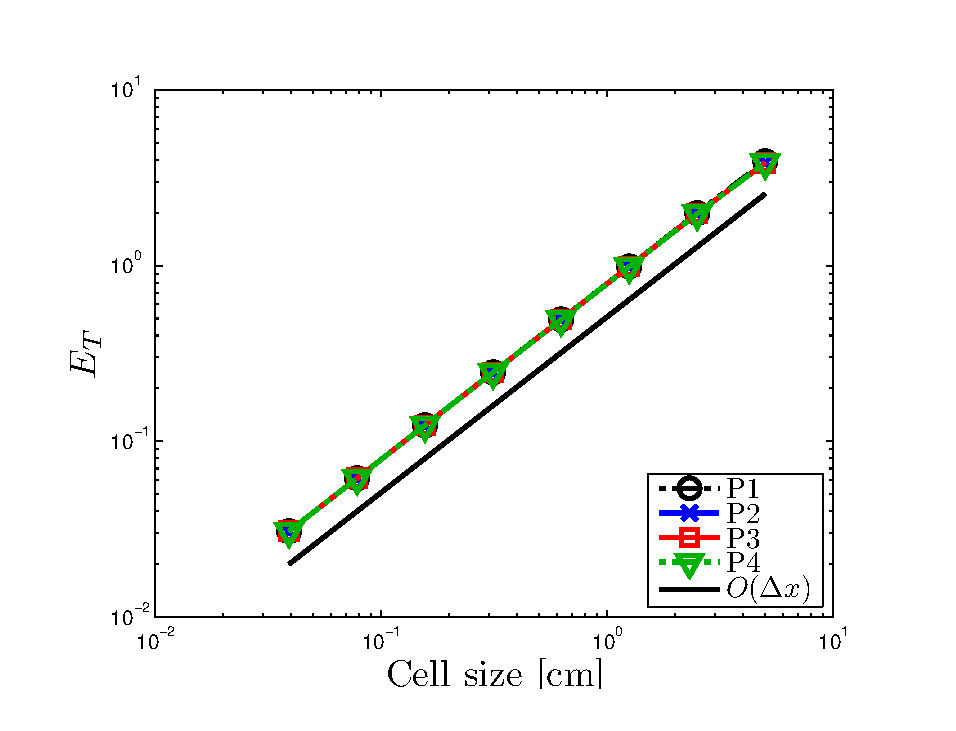
\includegraphics[width=10cm,trim=0.25in  0.2in 0.75in 0.5in,clip=true]{chapter6_grey_radtran/Dissertation_Data/MMS3_Constant_XS_SL_Gauss_temp_L2.pdf}
\caption{Convergence of $E_{T}$ for the SL Gauss scheme in problem MMS2.}
\label{fig:mms3_constant_gauss_temp}
\end{figure}

Regardless of DFEM interpolation point type or trial space degree, assuming cell-wise constant material properties limits spatial convergence of $E_{\phi}$ to at most second order.
Confirming our suspicion that assuming cell-wise constant material properties limit the convergence of $E_T$ as well, we plot the convergence of $E_T$ for the SL Lobatto scheme in \fig{fig:mms3_constant_lobatto_temp} and for the SL Gauss scheme in \fig{fig:mms3_constant_gauss_temp}.
Figures \ref{fig:mms3_constant_lobatto_temp}-\ref{fig:mms3_constant_gauss_temp} verify the hypothesis we developed while discussing our neutron transport results: assuming a cell-wise constant opacity limits $L^2$ convergence of temperature to at most first order in space, regardless of DFEM trial space degree.

Recalling that in \secref{sec:chapter3_variable_xs}, assuming a cell-wise constant cross section equal to the volumetric average cross section in a neutron transport pure absorber problem
resulted in a scheme that converged the cell average interaction rate, $E_{IR_A}$, $\propto 2P+1$, we now consider convergence of $E_{T_A}$, a quantity controlled by cell average interaction rates.
in \fig{fig:mms3_constant_lobatto_temp_A} and \fig{fig:mms3_constant_gauss_temp_A}.
Figure \ref{fig:mms3_constant_lobatto_temp_A} verifies that regardless of trial space degree, the SL Lobatto scheme assuming a cell-wise constant opacity for a problem with temperature or spatially varying opacities converges $E_{T_A}$ second order in space.
Likewise, \fig{fig:mms3_constant_gauss_temp_A} demonstrates the same is true for the SL Gauss scheme.
\begin{figure}[!hbp]
\centering
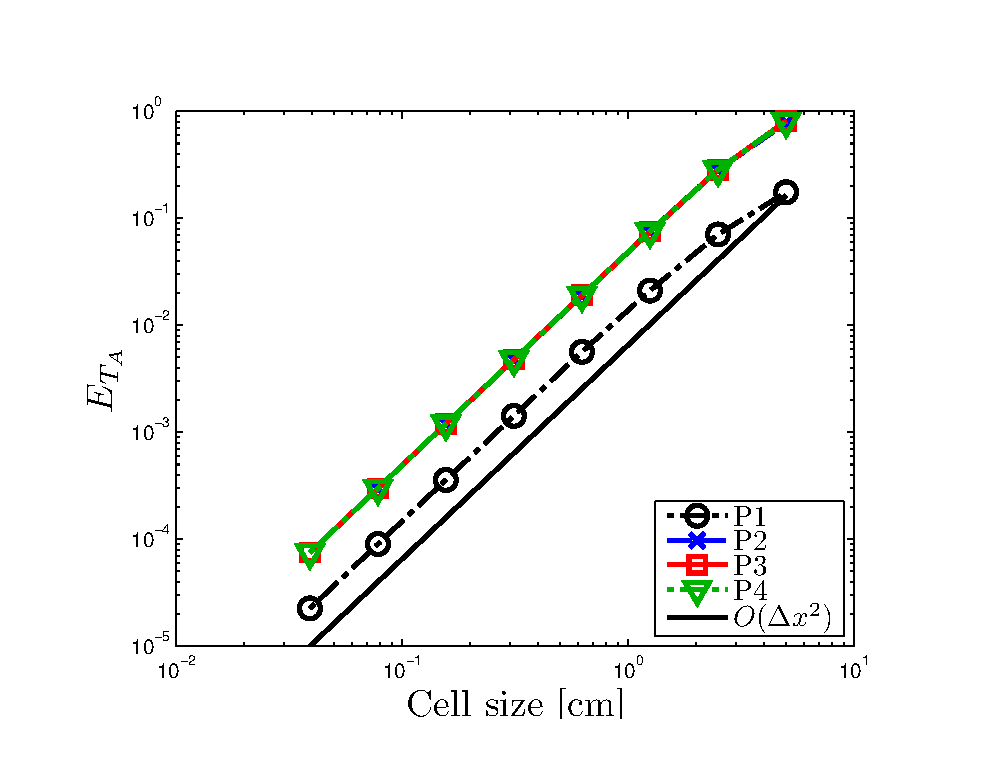
\includegraphics[width=9.5cm,trim=0.25in  0.2in 0.75in 0.5in,clip=true]{chapter6_grey_radtran/Dissertation_Data/MMS3_Constant_XS_SL_Lobatto_temp_A.pdf}
\caption{Convergence of $E_{T_A}$ for the SL Lobatto scheme in problem MMS2.}
\label{fig:mms3_constant_lobatto_temp_A}
\end{figure}
%
%
\begin{figure}[!htp]
\centering
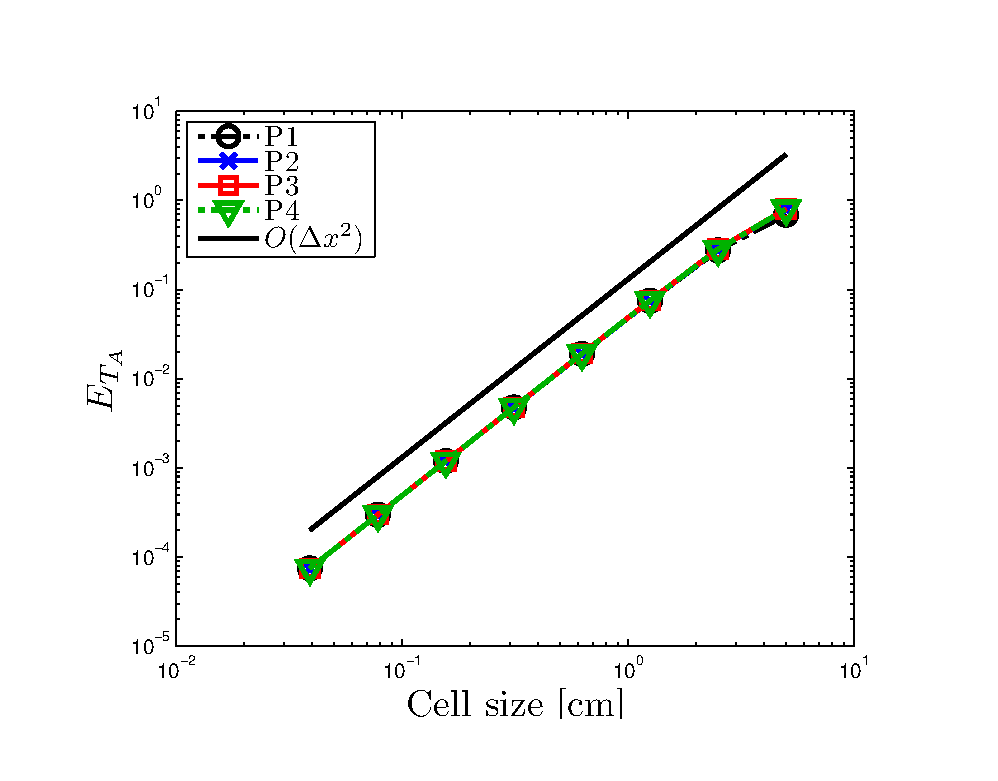
\includegraphics[width=9.5cm,trim=0.25in  0.2in 0.75in 0.5in,clip=true]{chapter6_grey_radtran/Dissertation_Data/MMS3_Constant_XS_SL_Gauss_temp_A.pdf}
\caption{Convergence of $E_{T_A}$ for the SL Gauss scheme in problem MMS2.}
\label{fig:mms3_constant_gauss_temp_A}
\end{figure}

We now consider the convergence of SLXS Lobatto and SLXS Gauss.  
First, we see that in \fig{fig:mms3_slxs_lobatto_e_phi}, SLXS Lobatto converges $E_{\phi} \propto P+1$, and in \fig{fig:mms3_slxs_gauss_e_phi}, SLXS Gauss converges $E_{\phi}$ $\propto P+1$ as well.
Moving on to the convergence of $E_T$, in \fig{fig:mms3_slxs_lobatto_e_t} SLXS Lobatto converges $E_T \propto P$, the same rate SL Lobatto converged $E_T$ for the TRT problem with constant material properties.  
In \fig{fig:mms3_slxs_gauss_e_t} SLXS Gauss converges $E_T$ very rapidly, and only the asymptotic convergence rate of linear and quadratic DFEM can be estimated, though both suggest SLXS Gauss converges $E_T \propto P+2$.
\begin{figure}[!hbp]
\centering
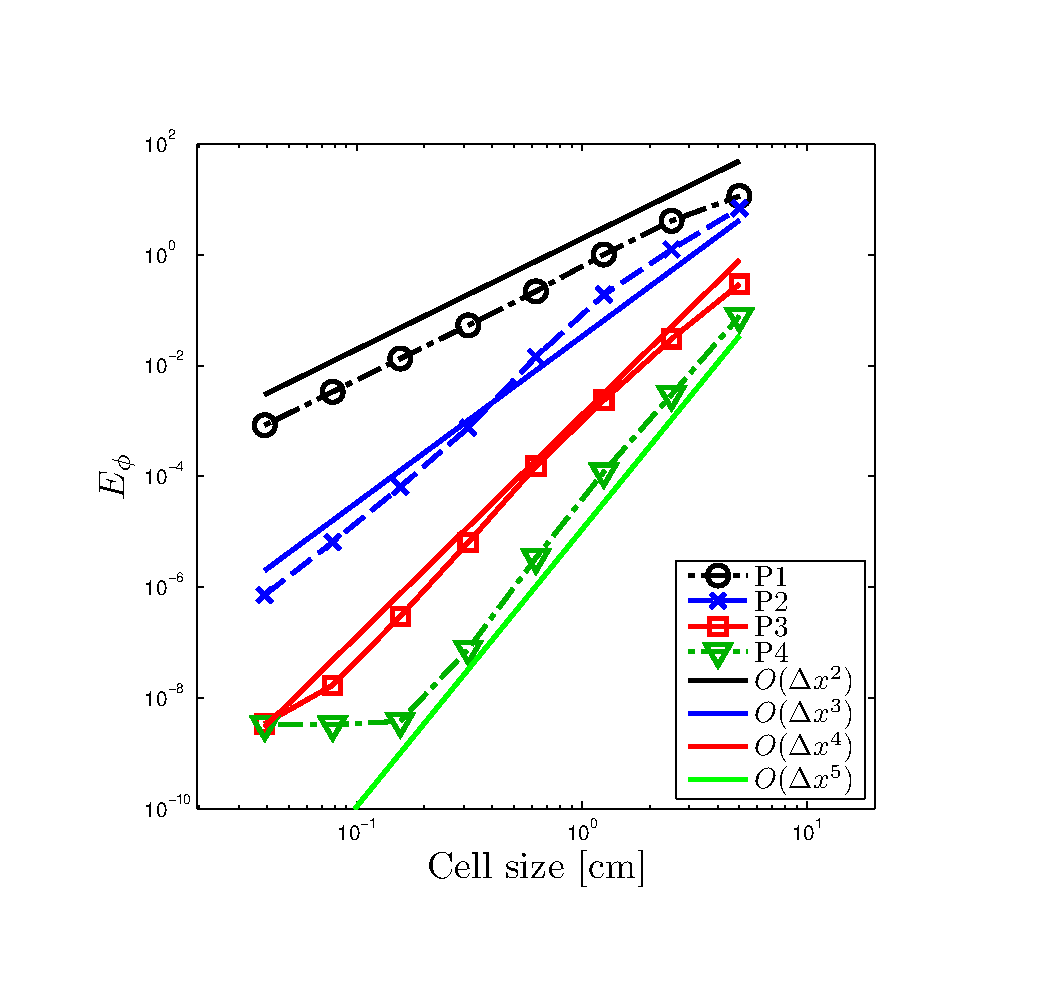
\includegraphics[width=10cm,trim=0.25in  0.25in 0.75in 0.75in,clip=true]{chapter6_grey_radtran/Dissertation_Data/MMS3_SLXS_Lobatto_phi_L2.pdf}
\caption{Convergence of $E_{\phi}$ for the SLXS Lobatto scheme in problem MMS2.}
\label{fig:mms3_slxs_lobatto_e_phi}
\end{figure}
%
%
\begin{figure}[!htp]
\centering
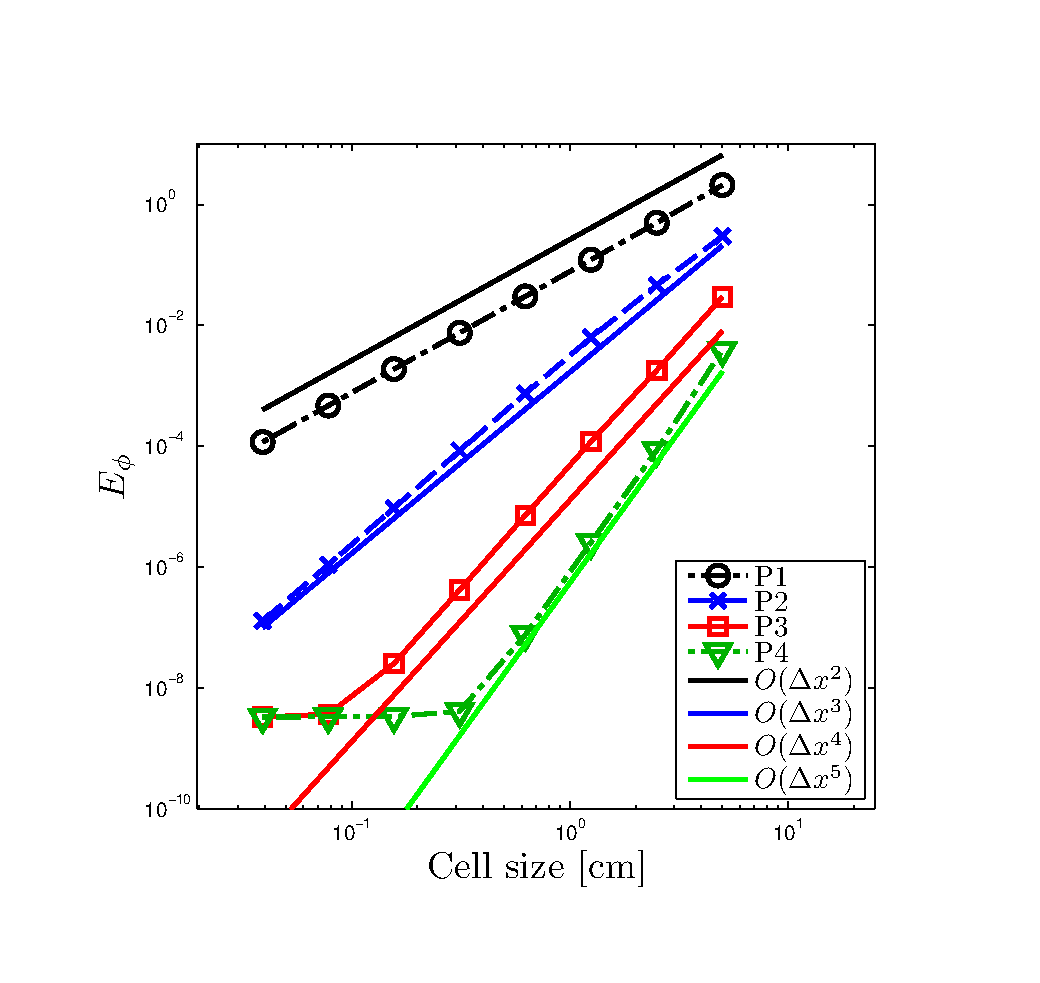
\includegraphics[width=10cm,trim=0.25in  0.25in 0.75in 0.75in,clip=true]{chapter6_grey_radtran/Dissertation_Data/MMS3_SLXS_Gauss_phi_L2.pdf}
\caption{Convergence of $E_{\phi}$ for the SLXS Gauss scheme in problem MMS2.}
\label{fig:mms3_slxs_gauss_e_phi}
\end{figure}
\begin{figure}[!hbp]
\centering
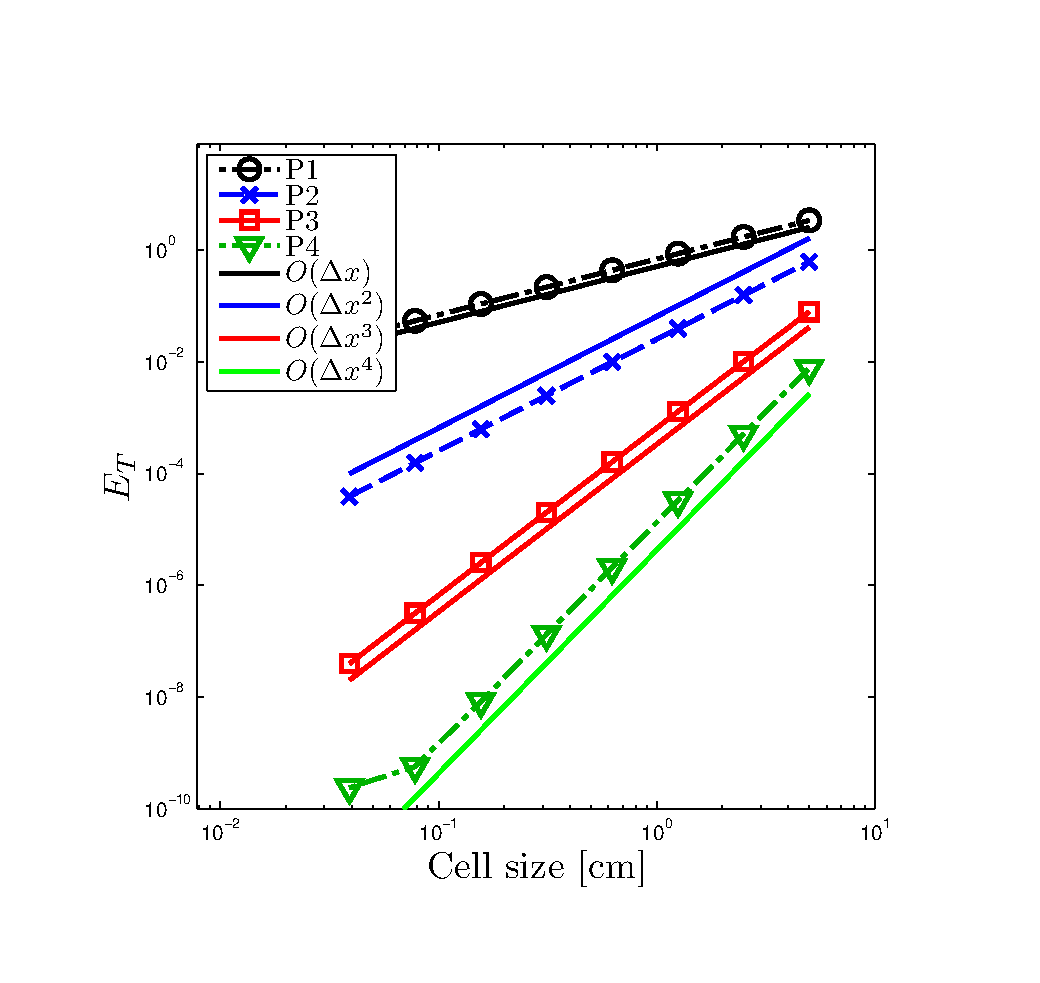
\includegraphics[width=10cm,trim=0.25in  0.25in 0.75in 0.75in,clip=true]{chapter6_grey_radtran/Dissertation_Data/MMS3_SLXS_Lobatto_temp_L2.pdf}
\caption{Convergence of $E_{T}$ for the SLXS Lobatto scheme in problem MMS2.}
\label{fig:mms3_slxs_lobatto_e_t}
\end{figure}
%
%
\begin{figure}[!htp]
\centering
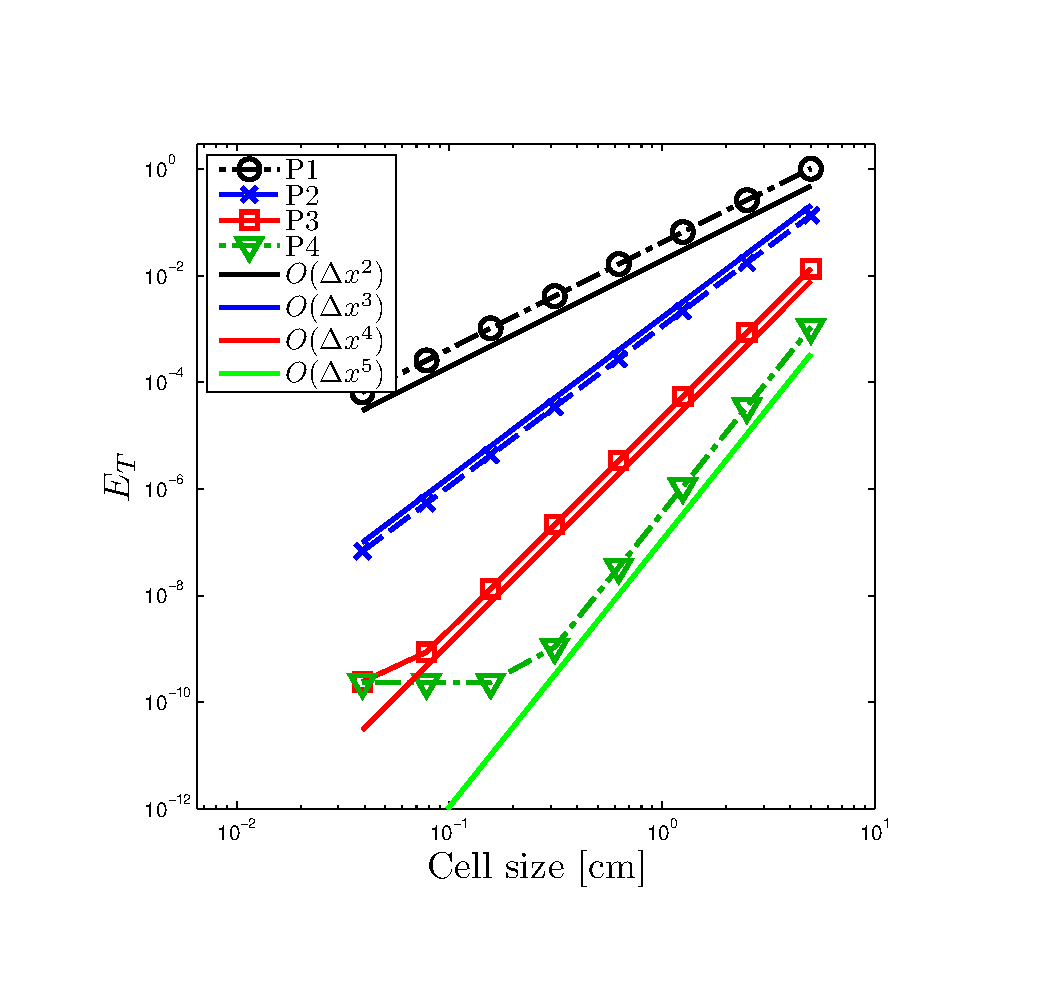
\includegraphics[width=9.5cm,trim=0.25in  0.25in 0.75in 0.75in,clip=true]{chapter6_grey_radtran/Dissertation_Data/MMS3_SLXS_Gauss_temp_L2.pdf}
\caption{Convergence of $E_{T}$ for the SLXS Gauss scheme in problem MMS2.}
\label{fig:mms3_slxs_gauss_e_t}
\end{figure}
%
%
%
\begin{figure}[!hbp]
\centering
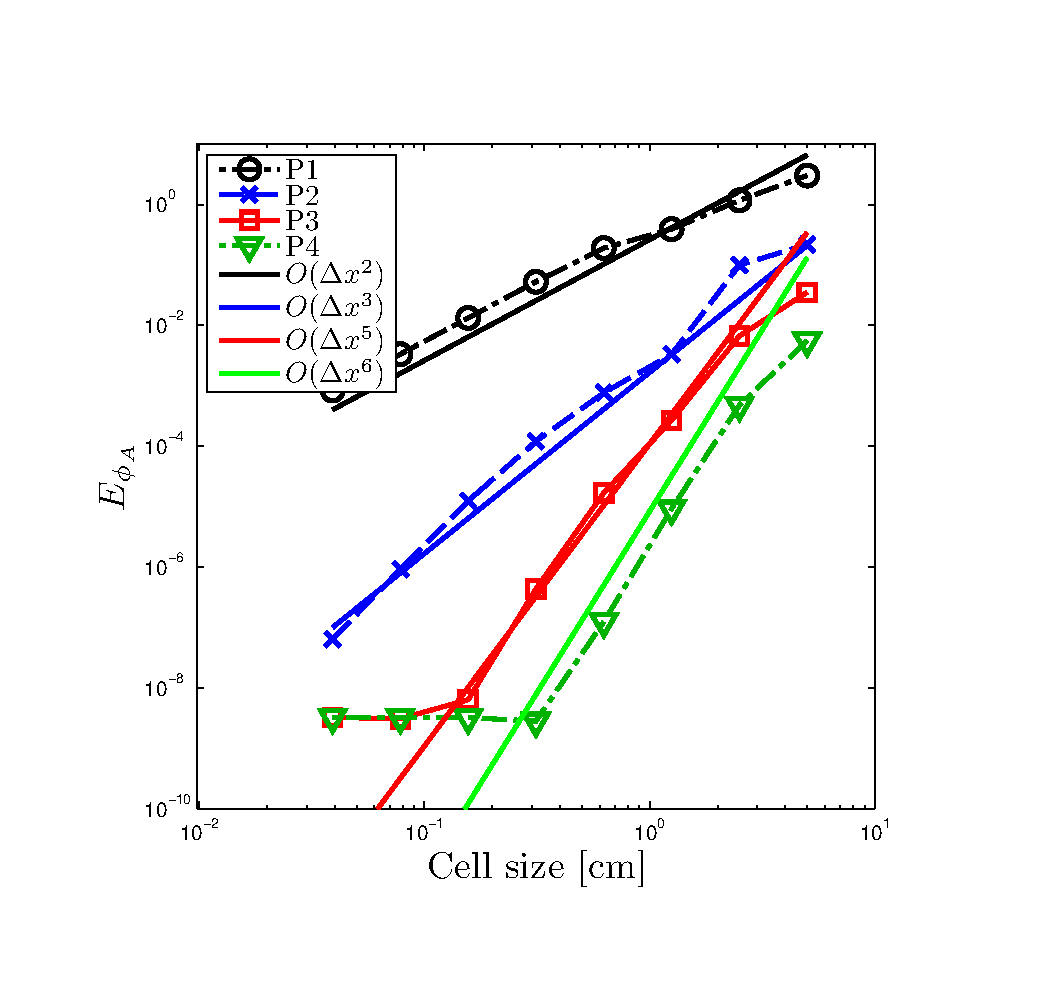
\includegraphics[width=9.5cm,trim=0.25in  0.4in 0.75in 0.75in,clip=true]{chapter6_grey_radtran/Dissertation_Data/MMS3_SLXS_SLXS_Lobatto_phi_A.pdf}
\caption{Convergence of $E_{\phi_A}$ for the SLXS Lobatto scheme in problem MMS2.}
\label{fig:mms3_slxs_lobatto_phi_a}
\end{figure}
%
%
\begin{figure}[!htp]
\centering
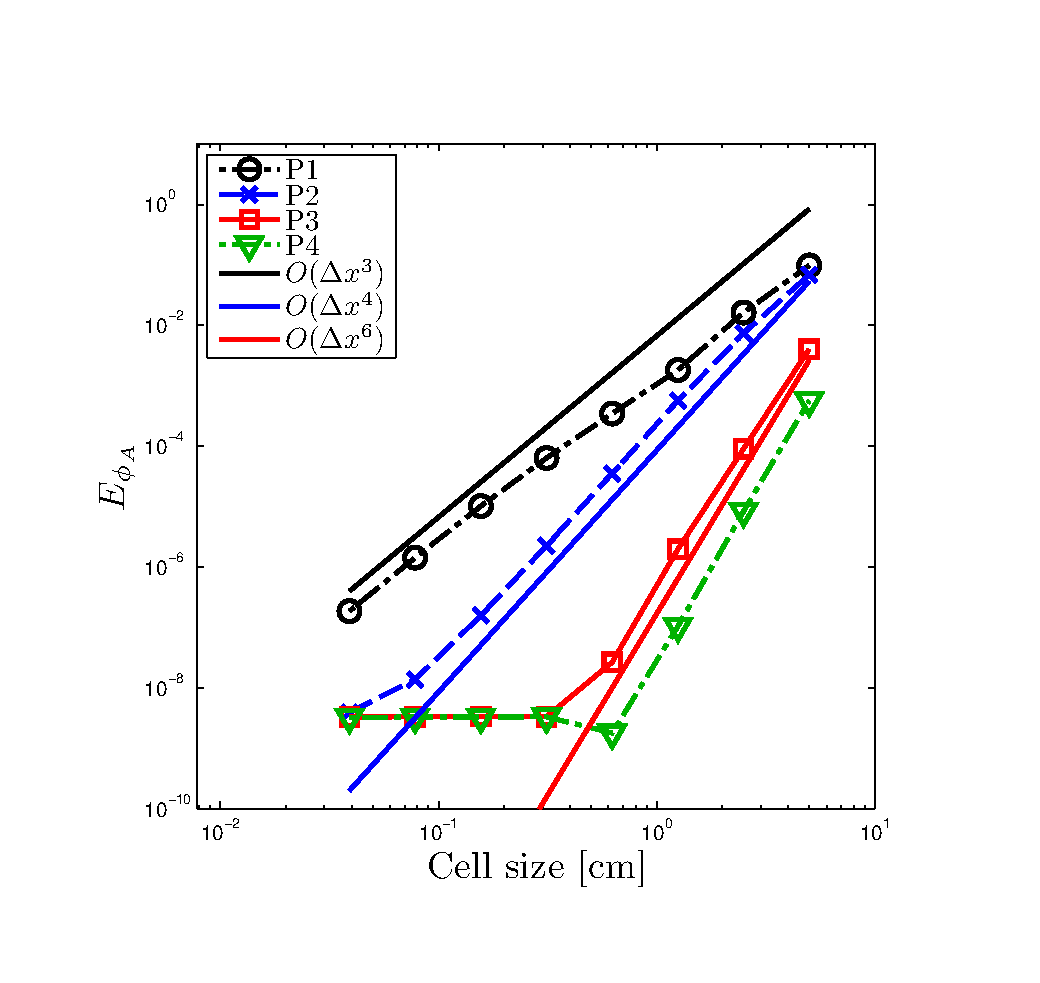
\includegraphics[width=10cm,trim=0.25in  0.25in 0.75in 0.75in,clip=true]{chapter6_grey_radtran/Dissertation_Data/MMS3_SLXS_Gauss_phi_A.pdf}
\caption{Convergence of $E_{\phi_A}$ for the SLXS Gauss scheme in problem MMS2.}
\label{fig:mms3_slxs_gauss_phi_a}
\end{figure}
\begin{figure}[!hbp]
\centering
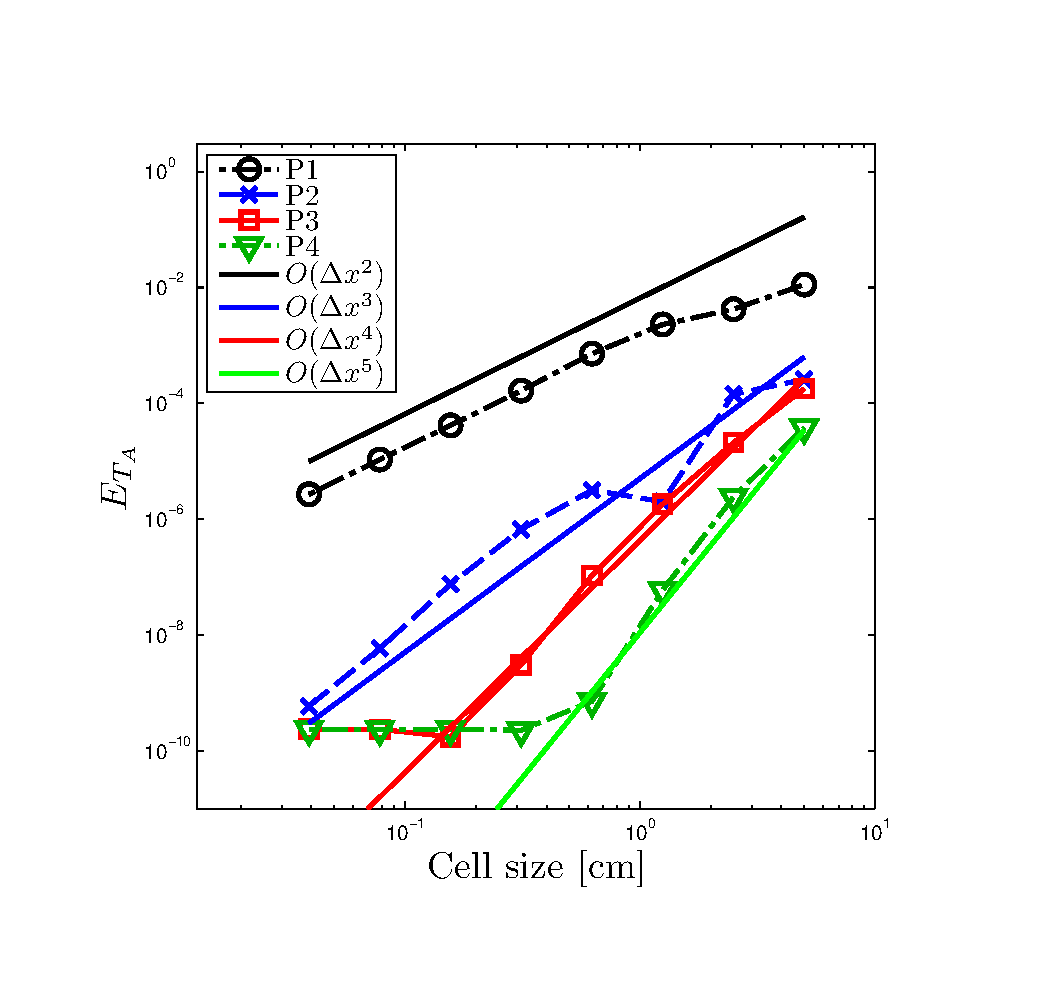
\includegraphics[width=10cm,trim=0.25in  0.25in 0.75in 0.75in,clip=true]{chapter6_grey_radtran/Dissertation_Data/MMS3_SLXS_Lobatto_temp_A.pdf}
\caption{Convergence of $E_{T_A}$ for the SLXS Lobatto scheme in problem MMS2.}
\label{fig:mms3_slxs_lobatto_t_a}
\end{figure}
%
%
\begin{figure}[!htp]
\centering
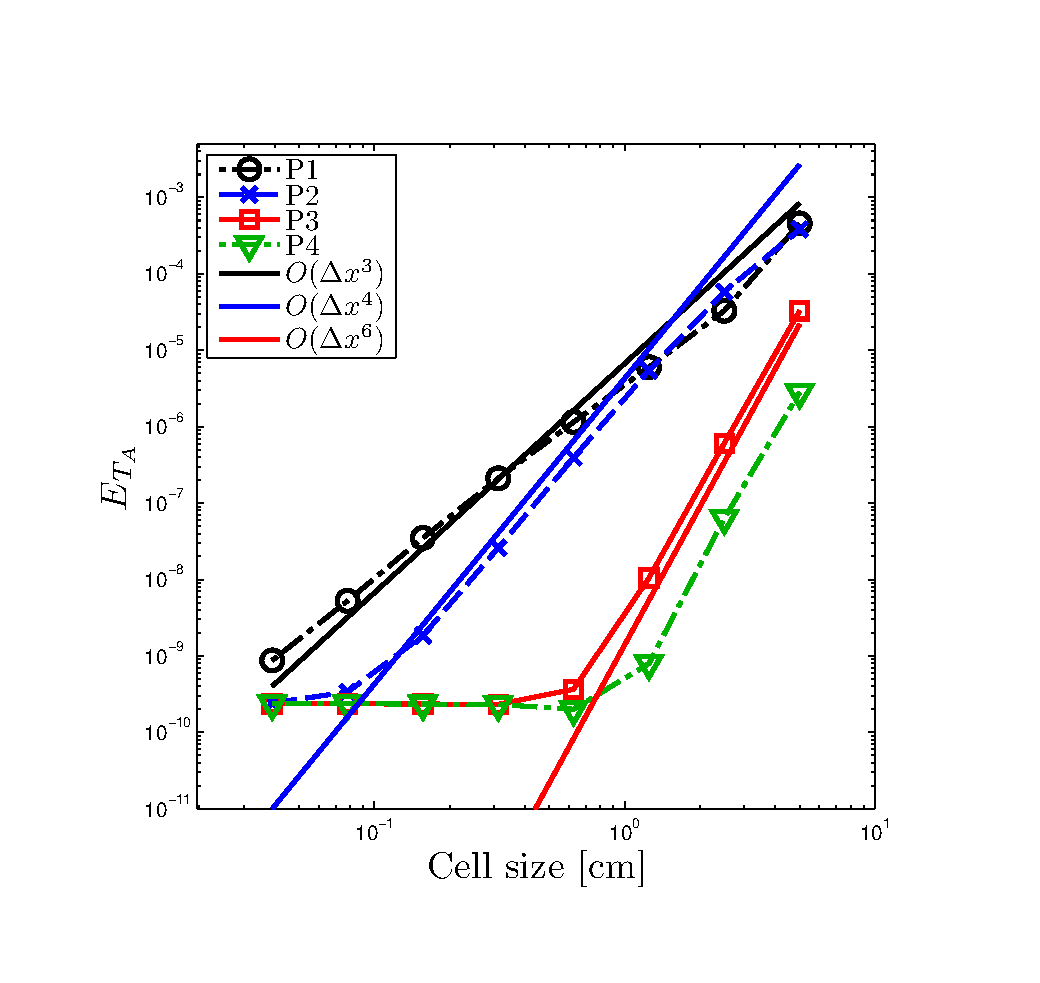
\includegraphics[width=10cm,trim=0.25in  0.25in 0.75in 0.75in,clip=true]{chapter6_grey_radtran/Dissertation_Data/MMS3_SLXS_Gauss_temp_A.pdf}
\caption{Convergence of $E_{T_A}$ for the SLXS Gauss scheme in problem MMS2.}
\label{fig:mms3_slxs_gauss_t_a}
\end{figure}

Focusing now on the convergence of cell average error quantities, we first consider $E_{\phi_A}$ for SLXS Lobatto and SLXS Gauss in \fig{fig:mms3_slxs_lobatto_phi_a} and \fig{fig:mms3_slxs_gauss_phi_a}, respectively.
Both SLXS Lobatto and SLXS Gauss converge $E_{\phi_A}$ at an order less than or at most equal to the order that their respective neutron transport analogs converged $E_{\psi_A}$.
However, since both methods require only a small amount of mesh refinement to reach an error level approximately equal to our temperature tolerance, it is difficult to establish with certainty the order of convergence of either method for higher $P$.
For completeness, we include convergence plots of $E_{T_A}$ for SLXS Lobatto and SLXS Gauss respectively in \fig{fig:mms3_slxs_lobatto_t_a} and \fig{fig:mms3_slxs_gauss_t_a}.
All we can definitively conclude from \figs{fig:mms3_slxs_lobatto_t_a}{fig:mms3_slxs_gauss_t_a} is that both SLXS Lobatto and SLXS Gauss experience increases in convergence of $E_{T_A}$ with increases in trial space degree.

In \figs{fig:mms1_tl_phi}{fig:mms3_slxs_gauss_t_a}, the plateauing of errors that appears in some plots is a result of our relative convergence tolerances for both temperature and angle integrated intensity. 
Given our convergence criteria, we might expect a plateau, $E_{T,min}$ of approximately
\benum
E_{T,min} \int_{x_{1/2} }^{x_{N_{cell}+1/2}}{ \epsilon_T \left[ F_t(t_{end}) W_T(x) \right] dx} \pep
\label{eq:err_plateau}
\eenum
Applying \eqt{eq:err_plateau} to MMS1, $E_{T,min} = 4.6\times 10^{-8}$, which is consistent with the location of the $E_T$ error plateau.
In \eqt{eq:err_plateau}, we are implicitly assuming that the error in $\phi$ is significantly less than the error in temperature. 
Alternatively, we could consider resulted generated with less stringent $\epsilon_T$ and $\epsilon_{\phi}$.
In \fig{fig:low_tol_slxs_gauss_temp} and \fig{fig:low_tol_slxs_lobatto_phi}, we give the results for $E_{T}$ convergence for the SLXS Gauss scheme and $E_{\phi}$ convergence for the SLXS Lobatto scheme for MMS2, but use $\epsilon_T=10^{-8}$ and $\epsilon_{\phi} = 10^{-10}$.  
Comparing the $E_T$ plateau in \fig{fig:low_tol_slxs_gauss_temp} of $\approx 5 \times 10^{-7}$ we see a factor of roughly 1000 increase compared to the plateau observed in \fig{fig:mms3_slxs_gauss_e_t}
 for the same quantity, equivalent to the relative relaxations of $\epsilon_T$ and $\epsilon_{\phi}$.
Likewise, the $E_{\phi}$ plateau of $\approx 10^{-5}$ in \fig{fig:low_tol_slxs_lobatto_phi} is roughly 1000 times greater than the same plateau observed in \fig{fig:mms3_slxs_lobatto_e_phi}.

\begin{figure}[!htp]
\centering
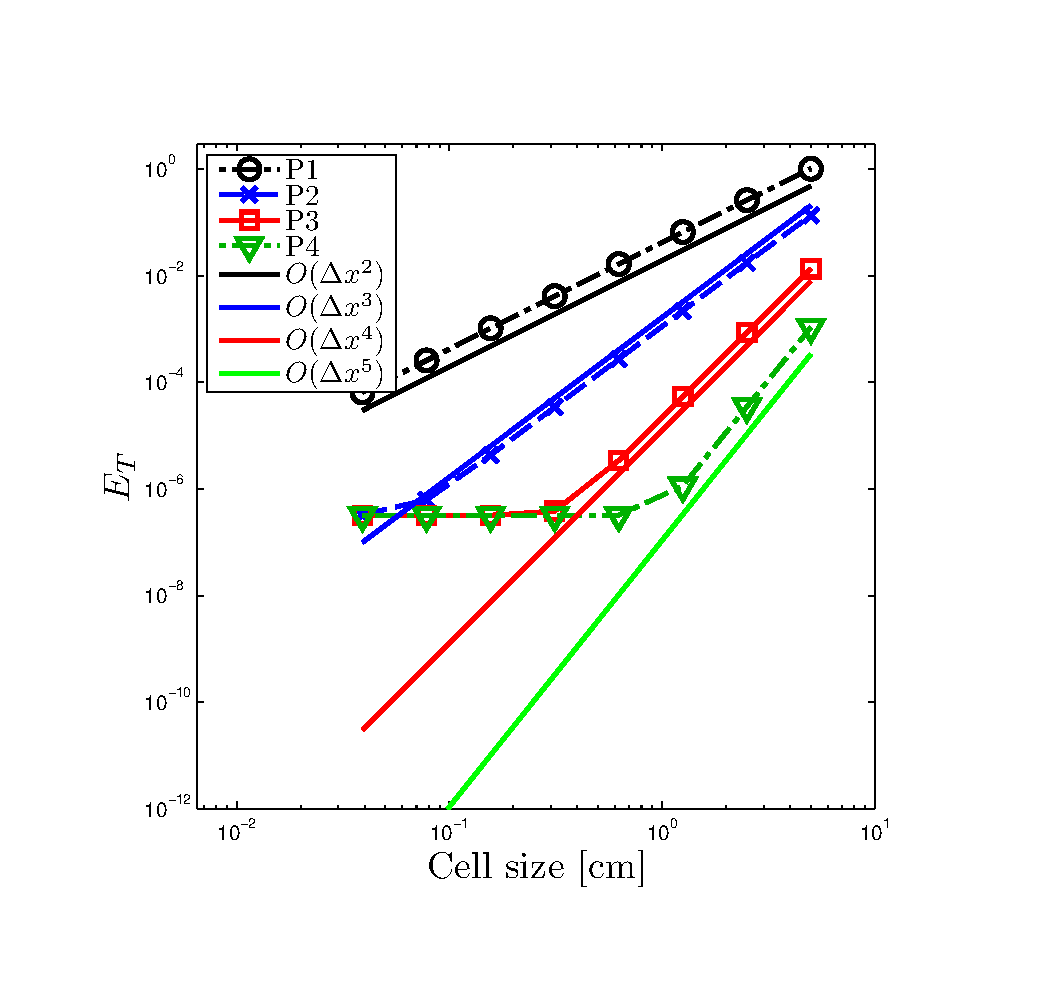
\includegraphics[width=9cm,trim=0.5in  0.5in 1in 0.75in,clip=true]{chapter6_grey_radtran/Dissertation_Data/MMS3_Low_Tol_SLXS_Gauss_temp_L2.pdf}
\caption{Convergence of $E_{T}$ for the SLXS Gauss scheme in problem MMS2 using $\epsilon_T = 10^{-8}$ and $\epsilon_{\phi}=10^{-10}$.}
\label{fig:low_tol_slxs_gauss_temp}
\end{figure}
%
%
\begin{figure}[!hbp]
\centering
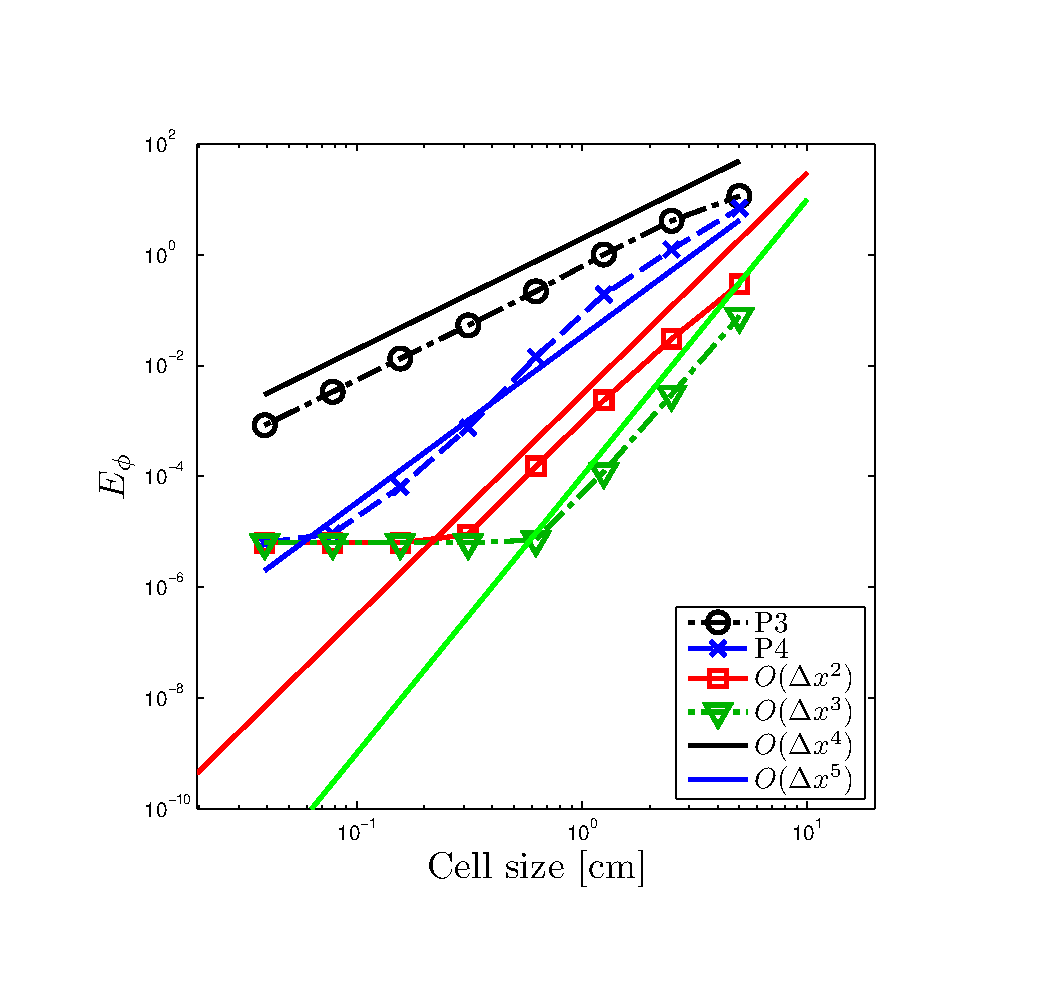
\includegraphics[width=9cm,trim=0.5in  0.5in 1in 0.75in,clip=true]{chapter6_grey_radtran/Dissertation_Data/MMS3_Low_Tol_SLXS_Lobatto_phi_L2.pdf}
\caption{Convergence of $E_{\phi}$ for the SLXS Lobatto scheme in problem MMS2 using $\epsilon_T = 10^{-8}$ and $\epsilon_{\phi}=10^{-10}$.}
\label{fig:low_tol_slxs_lobatto_phi}
\end{figure}

\subsubsection{Constant in Time - Trigonometric in Space - with Temperature Dependent Material Properties}

We now consider a problem that is constant in time and varies as a cosine in space with temperature dependent material properties.  
Though very similar to MMS2, we hope that by considering a truly steady state problem, we can study the spatial error of our DFEM schemes without temporal error interference.
We impose a solution of the form:
\beanum
M(\mu_d) &=& \frac{1}{4\pi} \\
W_I(x) &=& 19 \cos\left( \frac{\pi x}{2} \right) + 20 \pec \\
W_T(x) &=&  15 \cos\left( \frac{\pi x}{2}  \right) + 20 \pec \\
F(t) &=&  10
\eeanum
and define the following material properties:
\beanum
C_v &=& 0.1 + 0.2 T^2 \\
\sigma_a &=& \frac{5}{T^2} \\
\sigma_s &=& 0.01 \pep
\eeanum
Repeating as we have before, we first consider the convergence of $E_{\phi}$ for SLXS Lobatto and SLXS Gauss in \fig{fig:constant_time_lobatto_phi} and \fig{fig:constant_time_gauss_phi}.
\begin{figure}[!htp]
\centering
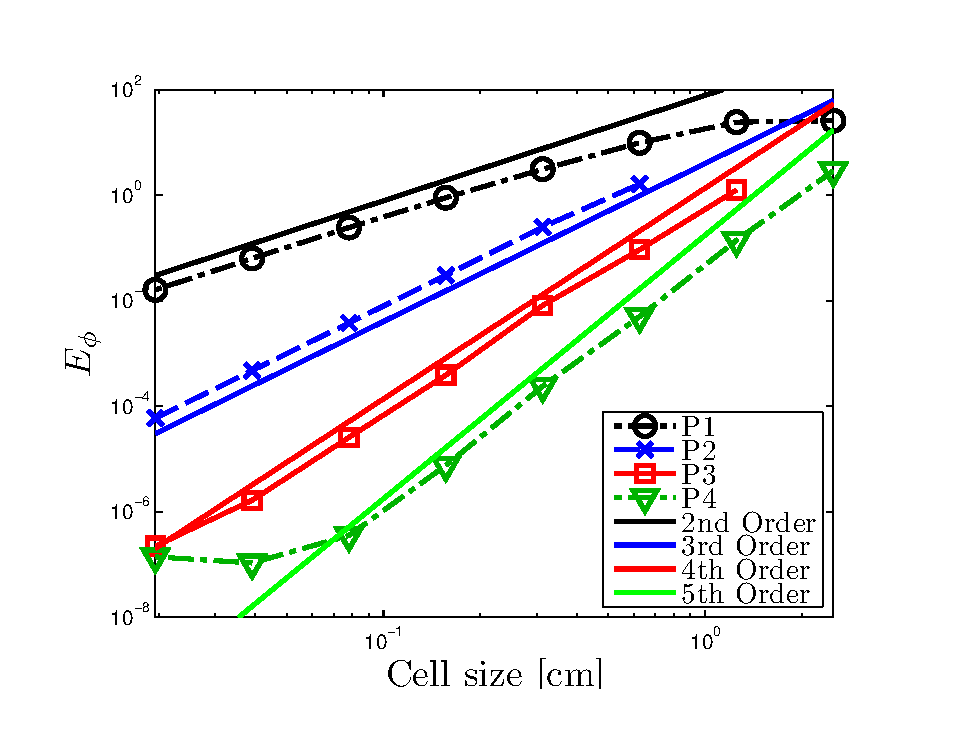
\includegraphics[width=10cm,trim=0.25in  0.2in 0.75in 0.5in,clip=true]{chapter6_grey_radtran/Dissertation_Data/Constant_Time_SLXS_Lobatto_phi_L2.pdf}
\caption{Convergence of $E_{\phi}$ for SLXS Lobatto scheme for steady state test problem.}
\label{fig:constant_time_lobatto_phi}
\end{figure}
%
%
\begin{figure}[!hbp]
\centering
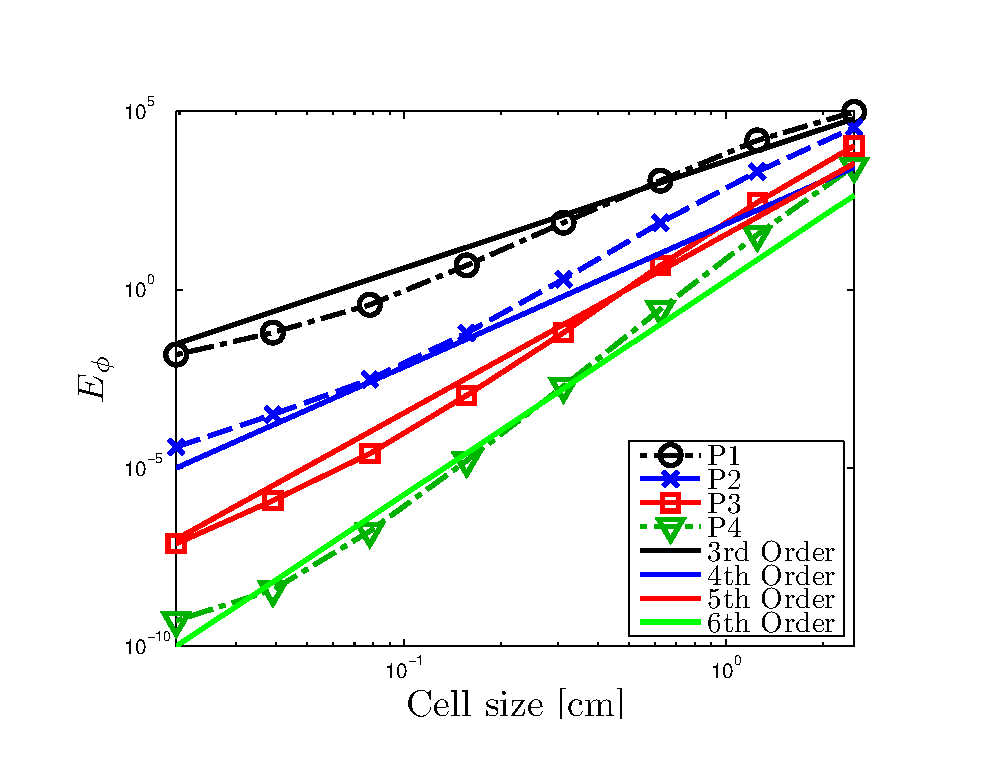
\includegraphics[width=10cm,trim=0.25in  0.2in 0.75in 0.5in,clip=true]{chapter6_grey_radtran/Dissertation_Data/Constant_Time_SLXS_Gauss_phi_L2.pdf}
\caption{Convergence of $E_{\phi}$ for SLXS Gauss scheme, for steady state test problem.}
\label{fig:constant_time_gauss_phi}
\end{figure}
As before, SLXS Lobatto converges $E_{\phi} \propto P+1$.  
However, SLXS Gauss appears to converges $E_{\phi} \propto P+2$.
It is not clear why SLXS Gauss convergence of $E_{\phi}$ increases when moving from the time dependent MMS1 and MMS2 problems to the steady-state test problem.

Now considering the convergence of $E_{T}$, the steady-state problem confirms SLXS Lobatto converges $E_T$ $\propto P$, shown in \fig{fig:constant_time_lobatto_t}, and SLXS Gauss converges $E_T \propto P+2$, as shown in \fig{fig:constant_time_gauss_t}.
\begin{figure}[!htp]
\centering
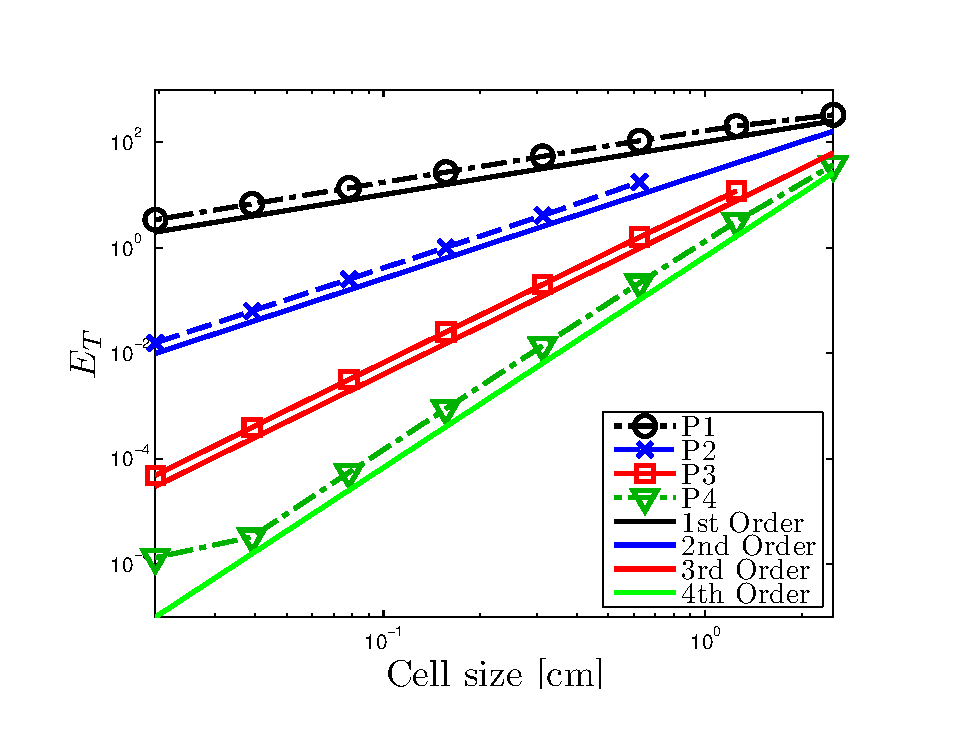
\includegraphics[width=10cm,trim=0.25in  0.2in 0.75in 0.5in,clip=true]{chapter6_grey_radtran/Dissertation_Data/Constant_Time_SLXS_Lobatto_temp_L2.pdf}
\caption{Convergence of $E_{T}$ for SLXS Lobatto scheme, for steady state test problem.}
\label{fig:constant_time_lobatto_t}
\end{figure}
%
\begin{figure}[!hbp]
\centering
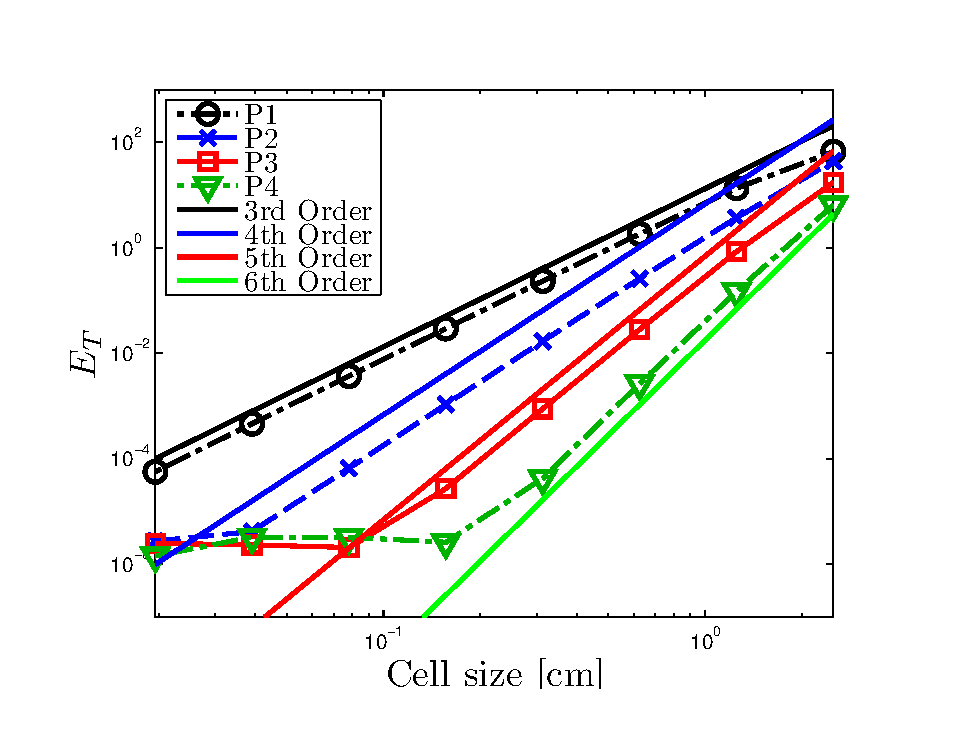
\includegraphics[width=9.5cm,trim=0.25in  0.2in 0.75in 0.5in,clip=true]{chapter6_grey_radtran/Dissertation_Data/Constant_Time_SLXS_Gauss_temp_L2.pdf}
\caption{Convergence of $E_{T}$ for SLXS Gauss scheme, for steady state test problem.}
\label{fig:constant_time_gauss_t}
\end{figure}

We now examine the convergence of $E_{\phi_A}$.  
The estimated order of convergence of $E_{\phi_A}$ in \fig{fig:constant_time_lobatto_phi_a} for SLXS Lobatto, appears to be $\propto 2P$, greater than the results from MMS1 and MMS2, but equal to what we would have hypothesized from neutron transport.  
%Figure \ref{fig:constant_time_lobatto_phi_a} and \fig{fig:mms3_slxs_lobatto_phi_a} giving different estimates of $E_{\phi_A}$ convergence is most likely due to a lack of data points available prior to reaching our iterative tolerances, preventing a clear inference of asymptotic convergence rate.
Similarly the convergence of $E_{\phi_A}$ for SLXS Gauss estimated in \fig{fig:constant_time_gauss_phi_a} appears to be greater, $\propto 2P+2$, than the SLXS Gauss order of convergence for $E_{\phi_A}$, $<2P+1$, given in \fig{fig:mms3_slxs_gauss_phi_a}.
\begin{figure}[!hbp]
\centering
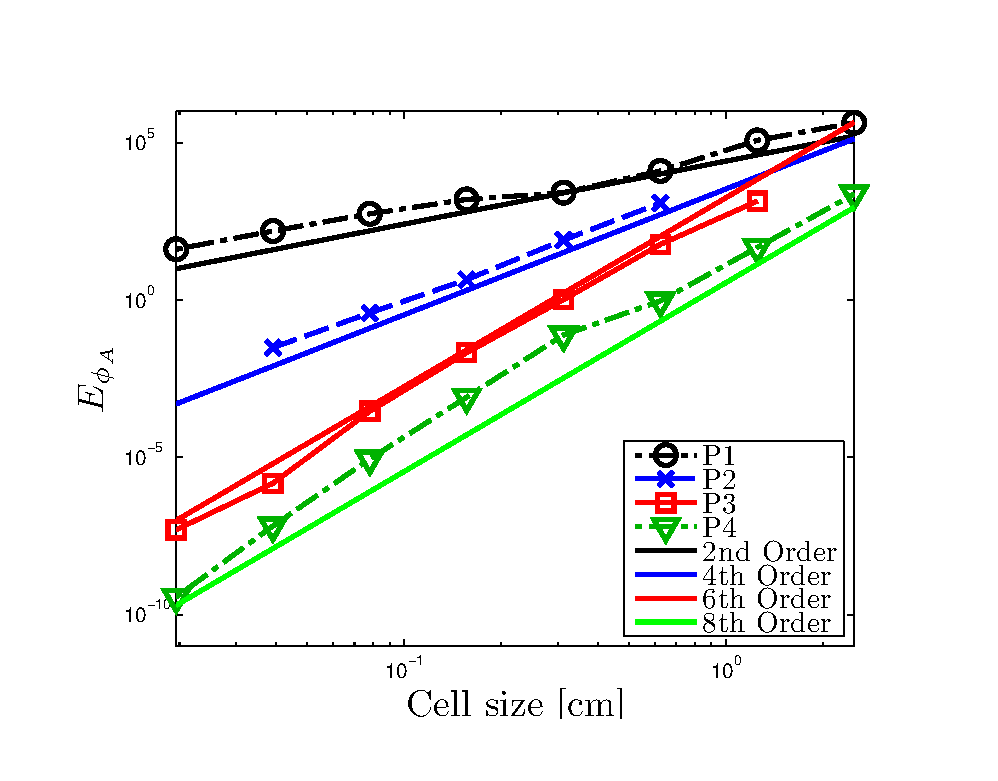
\includegraphics[width=10cm,trim=0.25in  0.2in 0.75in 0.5in,clip=true]{chapter6_grey_radtran/Dissertation_Data/Constant_Time_SLXS_Lobatto_phi_A.pdf}
\caption{Convergence of $E_{\phi_A}$ for SLXS Lobatto scheme, for steady state test problem.}
\label{fig:constant_time_lobatto_phi_a}
\end{figure}
%
%
\begin{figure}[!htp]
\centering
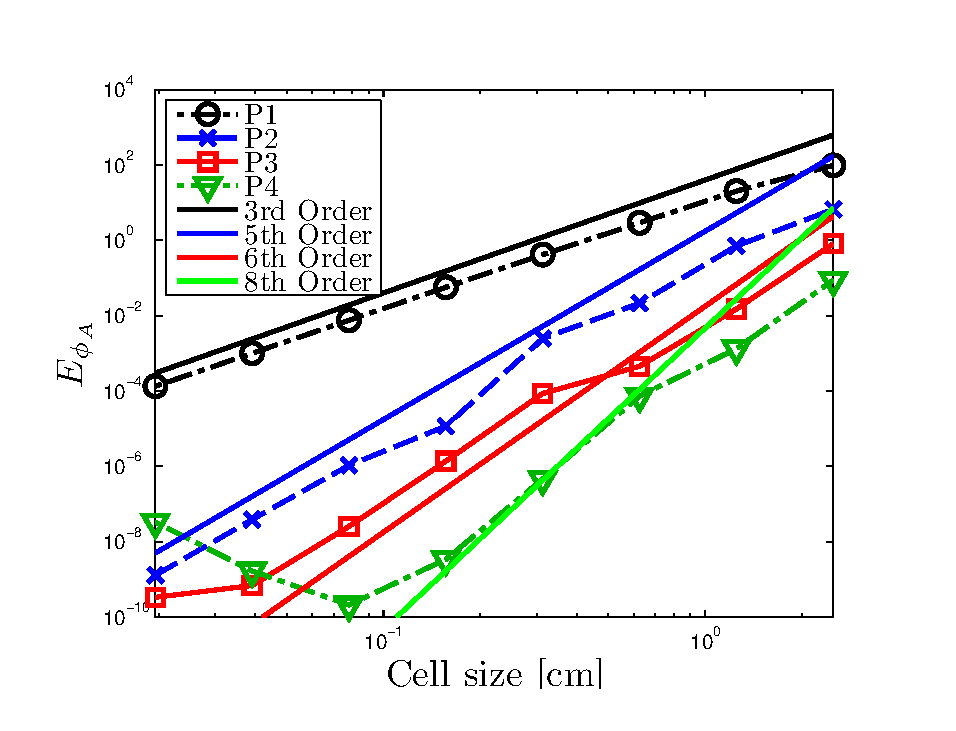
\includegraphics[width=10cm,trim=0.25in  0.2in 0.75in 0.5in,clip=true]{chapter6_grey_radtran/Dissertation_Data/Constant_Time_SLXS_Gauss_phi_A.pdf}
\caption{Convergence of $E_{\phi_A}$ for SLXS Gauss scheme, for steady state test problem.}
\label{fig:constant_time_gauss_phi_a}
\end{figure}

Finally, we consider the convergence of $E_{T_A}$.  
In \fig{fig:constant_time_lobatto_t_a} SLXS Lobatto converges $E_{T_A}$ $\propto 2P$, and in \fig{fig:constant_time_gauss_t_a}
SLXS Gauss converges $E_{T_A} \propto 2P+2$.  
Both of these convergence rates are higher than those observed in any of our previous MMS test problems.
The SLXS Lobatto $E_{T_A}$ convergence rate is equal to the SLXS Lobatto convergence rates for $E_{\psi_A}$ and $E_{IR_A}$, whereas the SLXS Gauss $E_{T_A}$ convergence rate is greater than any convergence rate observed for SLXS Gauss for neutron transport.
\begin{figure}[!htp]
\centering
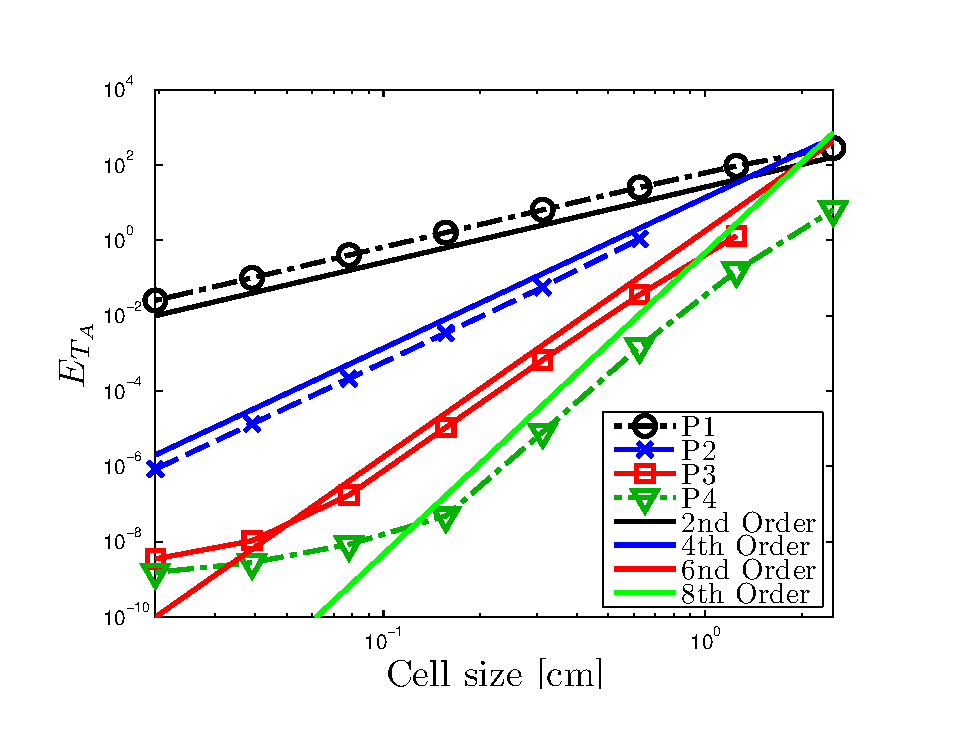
\includegraphics[width=9.5cm,trim=0.25in  0.25in 0.75in 0.5in,clip=true]{chapter6_grey_radtran/Dissertation_Data/Constant_Time_SLXS_Lobatto_temp_A.pdf}
\caption{Convergence of $E_{T_A}$ for SLXS Lobatto scheme, for steady state test problem.}
\label{fig:constant_time_lobatto_t_a}
\end{figure}
%
%
\begin{figure}[!htp]
\centering
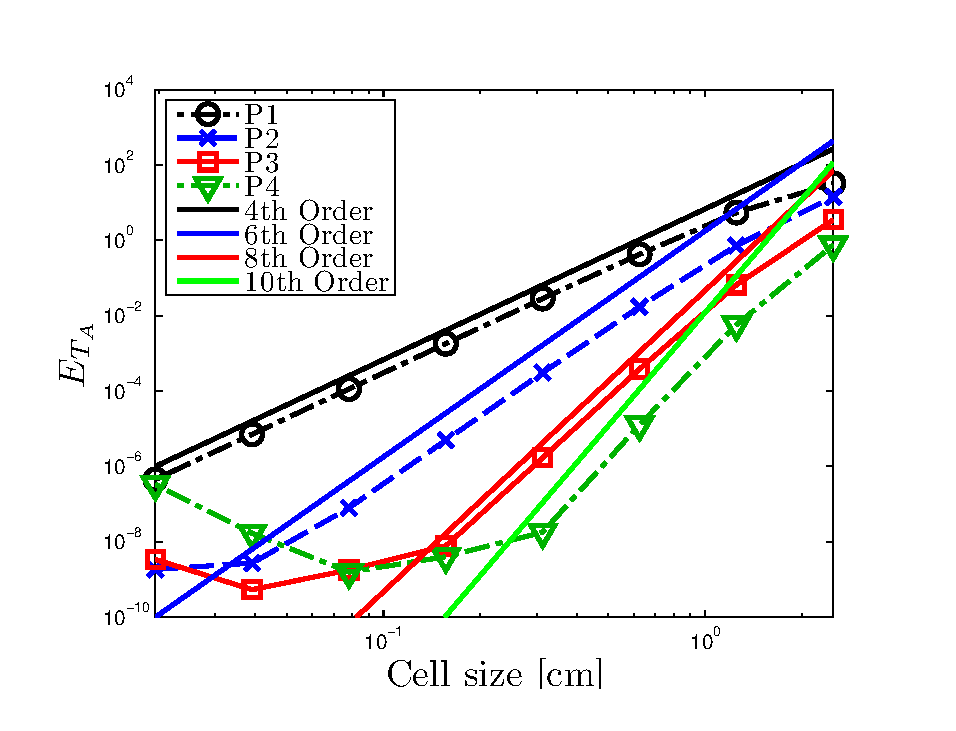
\includegraphics[width=9.5cm,trim=0.25in  0.25in 0.75in 0.5in,clip=true]{chapter6_grey_radtran/Dissertation_Data/Constant_Time_SLXS_Gauss_temp_A.pdf}
\caption{Convergence of $E_{T_A}$ for SLXS Gauss scheme, for steady state test problem.}
\label{fig:constant_time_gauss_t_a}
\end{figure}

\newpage

\subsubsection{Constant in Space - Trigonometric in Time}
\label{sec:time_convergence}


We now verify the asymptotic order of convergence of each SDIRK scheme: IE,  SDIRK 2-2, and SDIRK 3-3, as a function of time step size.
To simplify the process, we consider a problem with constant spatial dependence:
\beanum
M(\mu_d) &=& \frac{1}{4\pi} \\
W_I(x) &=& \frac{10}{4\pi} \\
W_T(x) &=&  10 \\
F(t) &=& 45 \cos\left( \pi t \right) + 46 \pec
\eeanum
$t \in[0,1]$, $\sigma_s = 0.1$, $\sigma_a = 2.5$, $C_v = 0.2$, $x\in[0,10]$ discretized with 10 equally spaced cells.  Convergence of $E_{\phi}$ as a function of $\Delta t$ for the IE, 2-2, and 3-3 time differencing schemes is given in \fig{fig:e_phi_time}.
As expected, IE converges 1st order in time, SDIRK 2-2 converges second order, and SDIRK 3-3 converges third order in time.
The same data for temperature is given in \fig{fig:big_dt}.  
Though the SDIRK 2-2 and SDIRK 3-3 schemes are always more accurate than IE, much smaller time steps were required for SDIRK  2-2 and SDIRK 3-3 to demonstrate their respective asymptotic orders of convergence for $E_T$ than were required to reach asymptotic convergence of $E_{\phi}$ with respect to time step size.
\begin{figure}[!htp]
\centering
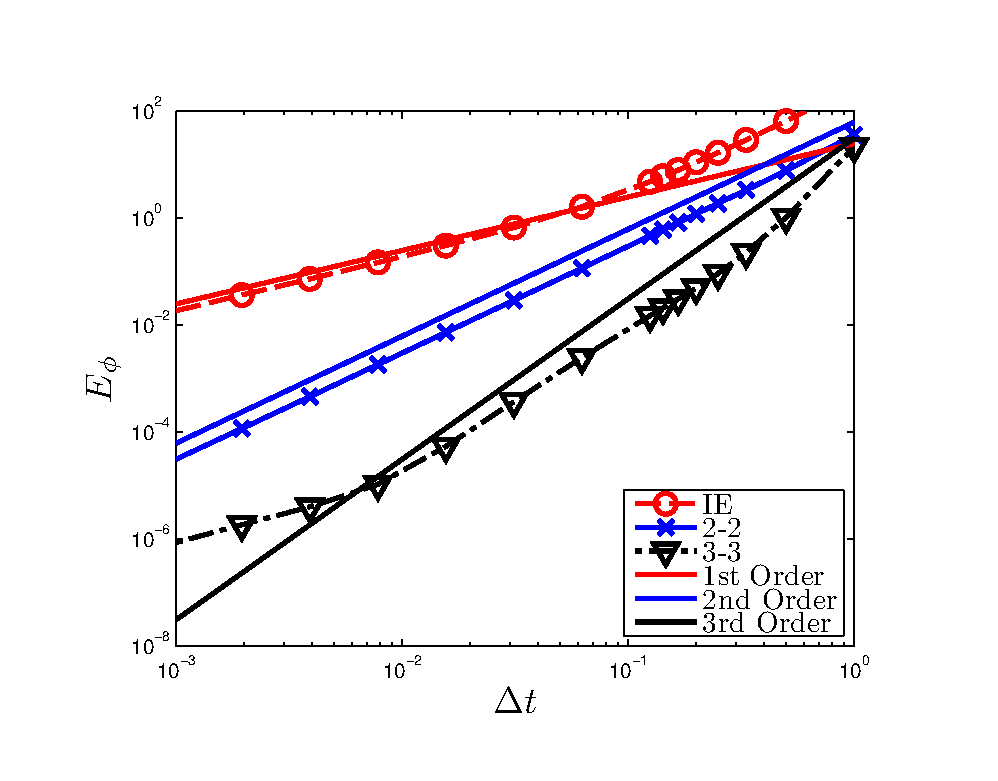
\includegraphics[width=12cm,trim=0.25in  0.2in 0.75in 0.5in,clip=true]{chapter6_grey_radtran/Dissertation_Data/Time_Integrators_Convergence_Phi.pdf}
\caption{Convergence of $E_{\phi}$ for different time integrators as a function of $\Delta t$.}
\label{fig:e_phi_time}
\end{figure}
\begin{figure}[!htp]
\centering
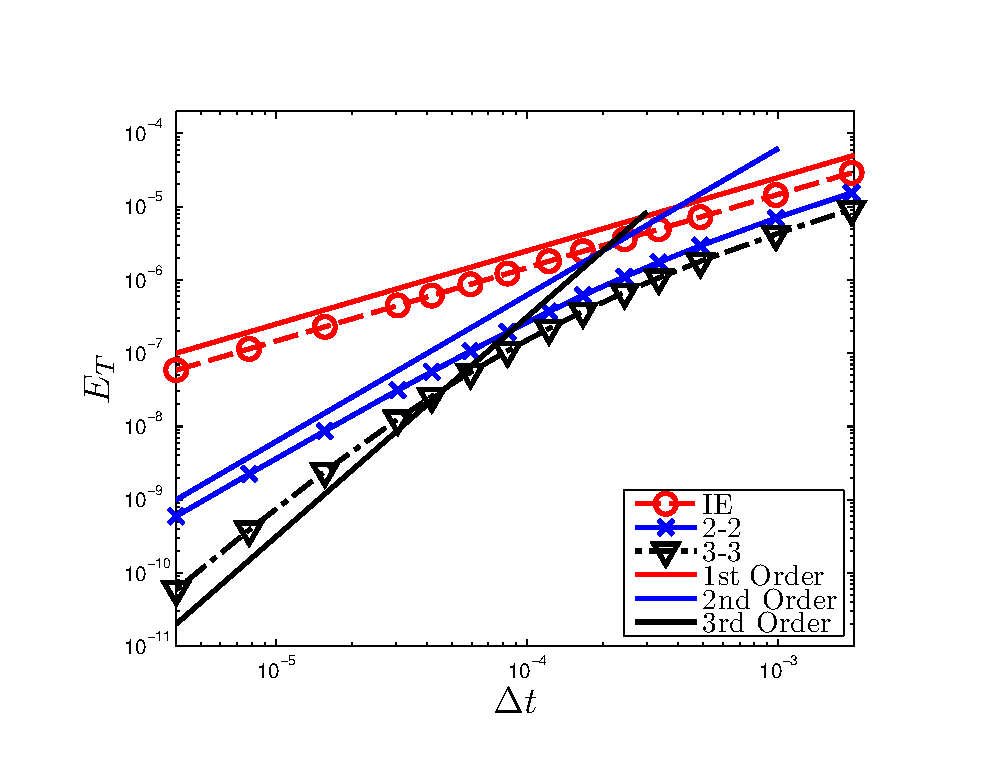
\includegraphics[width=12cm,trim=0.25in  0.2in 0.75in 0.5in,clip=true]{chapter6_grey_radtran/Dissertation_Data/Time_Integrators_Convergence_Temperature.pdf}
\caption{Convergence of $E_{T}$ for different time integrators as a function of $\Delta t$.}
\label{fig:big_dt}
\end{figure}

\pagebreak

\section{Thermal Radiative Transfer Simulations without Analytic Solutions}
\label{sec:marshak_waves}

We now consider two Marshak wave test problems.
In thermal radiative transfer problems, at low temperatures, materials are generally optically thick and emit very few photons, behaving like pure absorbers.
However, as the material heats up, its optical thickness decreases, photon emission increases, and the problem becomes very diffusive.
Marshak wave test problems, problems that begin with a cold material that is heated by an incident photon beam, are extremely challenging for discrete ordinates transport spatial discretizations, requiring methods that are accurate in both transport effects (cold material) and diffusive (heated material) regimes, and that can handle rapid variations in material properties.

The first problem, originally described by Ober and Shadid for radiative diffusion \cite{ober_shadid}, arbitrarily sets $a=c=C_v=1$, and as such, we will refer to it as the ``unity'' Marshak wave problem. 
Originally proposed in 1960 by Petschek and Williamson \cite{physical_marshak}, but considered more recently in \cite{negative_trt,time_adaptive_diffusion}, our second Marshak wave problem has a similar opacity dependence, $\sigma_a \propto T^{-3}$, as the unity Marshak wave problem, but uses physical units.  
We thus refer to the second Marshak wave problem as the physical Marshak wave problem.

\subsection{Unity Marshak Wave Problem}

%The unity Marshak wave problem consists of an initially cold slab that is heated from the left by an incident radiation intensity, with a vacuum boundary condition on the right.
Given as a radiative diffusion problem, we adapt the radiative diffusion problem of \cite{ober_shadid} to discrete ordinates thermal radiative transfer by interpreting the left boundary to be a unit isotropic incident current.
The physical domain is $x\in[0,1]$ and we advance the solution from $t=0$ to $t=1$.
Initially, the slab is in thermal equilibrium, and $T=\left( 10^{-5} \right)^{1/4}$.
There is no scattering, $\sigma_s = 0$, and the absorption opacity is temperature dependent, $\sigma_a = \frac{1}{T^3}$.
Like most thermal radiative transfer problems, no analytic solution exists.  
As such, we focus on qualitative comparisons of how DFEM trial space degree, mesh refinement, and time step refinement affect the radiation energy density and material temperature solutions.

We use an initial mesh of 20 cells, but also consider results using meshes of 80, 320, and 1280 cells.
Unless otherwise noted, for all simulations we use the SDIRK 2-2 time discretization.
We begin with a minimum time step of $\Delta t = 5\times 10^{-4}$ and increase the time step size by 10\% until we reach a maximum time step size of $\Delta t = 10^{-2}$.
For our time refinement studies, we divide the minimum and maximum time step sizes both by a factor of 4, 16, or 64.
We consider linear, quadratic, cubic and quartic SLXS Lobatto and SLXS Gauss schemes.
To demonstrate that assuming a cell-wise constant opacity results in a bladed  TRT temperature solution, we also consider linear SL Lobatto with a cell-wise volumetric average opacity.

We first investigate the effect of assuming a cell-wise constant opacity.  
Figure \ref{fig:bladed_rad_profile} shows the linear SL Lobatto radiation energy density solution at $t=1.0$.
Except for the effects of a very coarse spatial mesh when using 20 cells, the radiation energy density solution is effectively smooth, and comparable to the results published in \cite{ober_shadid}.  
The full temperature solution is shown in \fig{fig:bladed_t_profile_full}.
Clearly, the large, non-monotonic discontinuities (blading) observed in the neutron transport interaction rate profile are present in the TRT temperature profile.
In \fig{fig:bladed_t_profile_full}, mesh refinement reduces the magnitude of the temperature solution blading but does not eliminate the phenomena.
To emphasize that blading is not eliminated with mesh refinement, consider \fig{fig:bladed_t_profile_zoom}, that zooms in on the material temperature solution near the Marshak wavefront.
\begin{figure}[!htp]
\centering
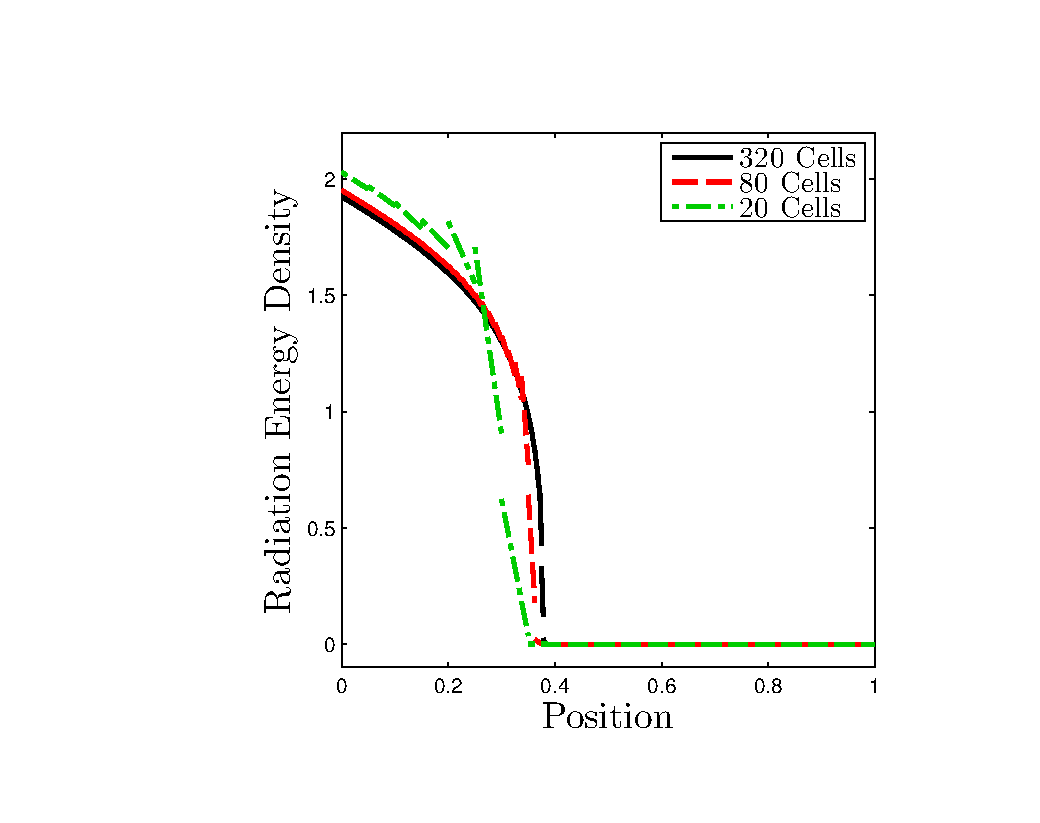
\includegraphics[width=9.5cm,trim=1.2in  0.2in 0.75in 0.5in,clip=true]{chapter6_grey_radtran/Dissertation_Data/Reorder_Blading_Radiation_Full_MultiCell.pdf}
\caption{Linear SL Lobatto radiation solution for the unity Marshak wave problem assuming cell-wise constant volumetric averaged opacities.}
\label{fig:bladed_rad_profile}
\end{figure}
%
%
\begin{figure}[!hbp]
\centering
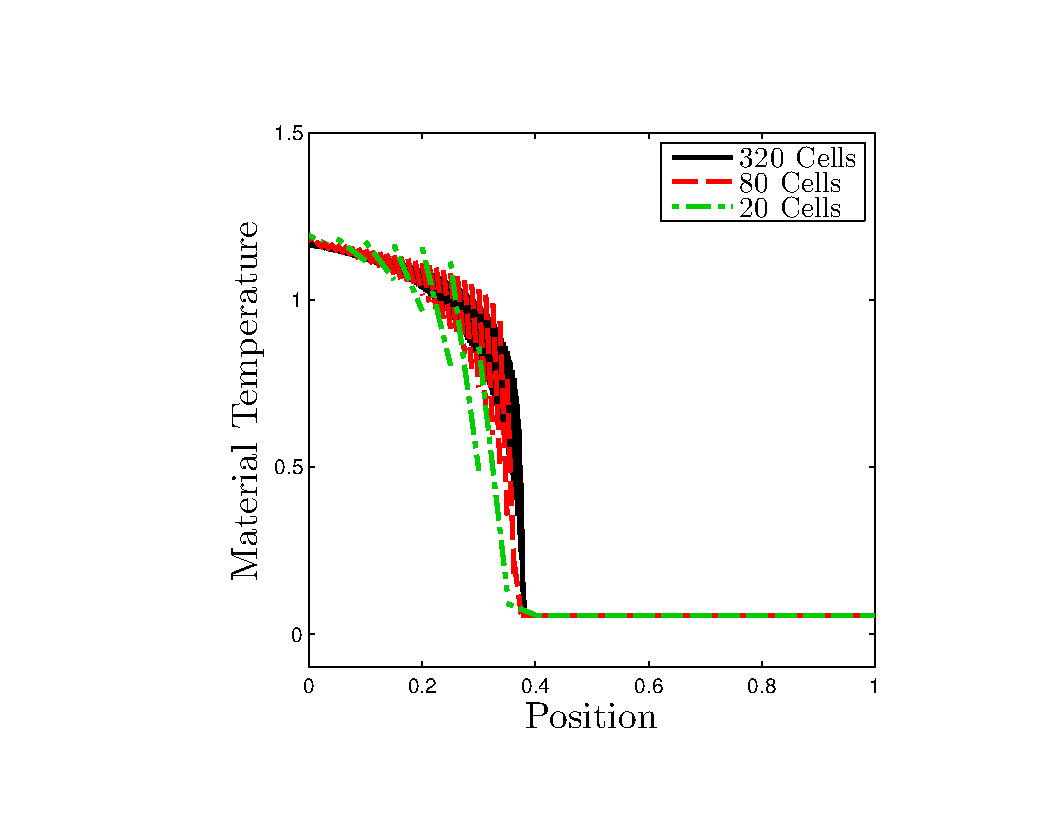
\includegraphics[width=9.5cm,trim=1.2in  0.2in 0.75in 0.5in,clip=true]{chapter6_grey_radtran/Dissertation_Data/Reorder_Blading_Temperature_Full_MultiCell.pdf}
\caption{Linear SL Lobatto temperature solution for the unity Marshak wave problem assuming cell-wise constant volumetric averaged opacities.}
\label{fig:bladed_t_profile_full}
\end{figure}
%
%
\begin{figure}[!htp]
\centering
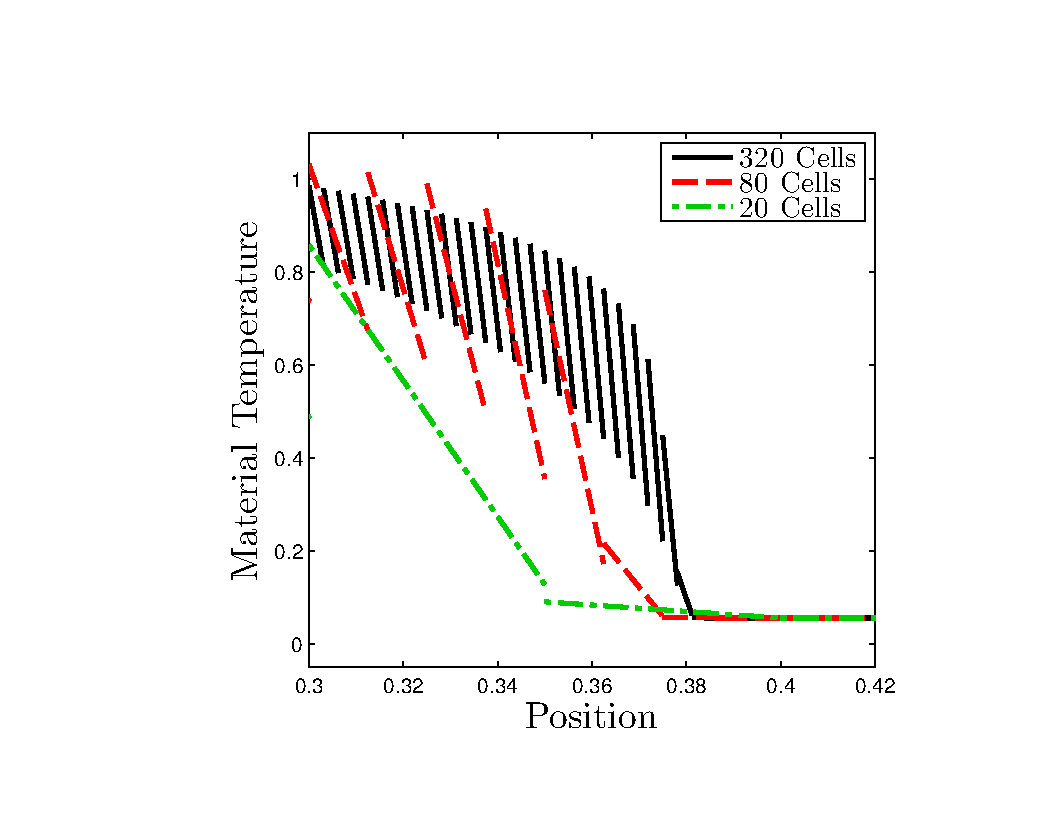
\includegraphics[width=9.5cm,trim=1.2in  0.2in 0.75in 0.5in,clip=true]{chapter6_grey_radtran/Dissertation_Data/Reorder_Blading_Temperature_Zoom_MultiCell.pdf}
\caption{Linear SL Lobatto temperature solution for the unity Marshak wave problem near the wavefront.}
\label{fig:bladed_t_profile_zoom}
\end{figure}
Clearly, \fig{fig:bladed_t_profile_full} and \fig{fig:bladed_t_profile_zoom}, in addition to the limited order of convergence results of \fig{fig:mms3_constant_lobatto_temp} and \fig{fig:mms3_constant_gauss_temp} demonstrate that the assumption of a cell-wise constant opacity is not appropriate for thermal radiative transfer simulations with temperature dependent material properties.

For comparison, consider the linear SLXS Lobatto radiation energy density solution in \fig{fig:linear_slxs_full_rad} and the temperature solution in \fig{fig:linear_slxs_full_temp}, computed using 80 mesh cells.
Visually, there is little difference between the SL Lobatto and SLXS Lobatto angle integrated intensity solutions.
However, this is not the case when examining the material temperature solutions.  
Unlike \fig{fig:bladed_t_profile_full}, \fig{fig:linear_slxs_full_temp} does not exhibit any blading.

%
\begin{figure}[!hbp]
\centering
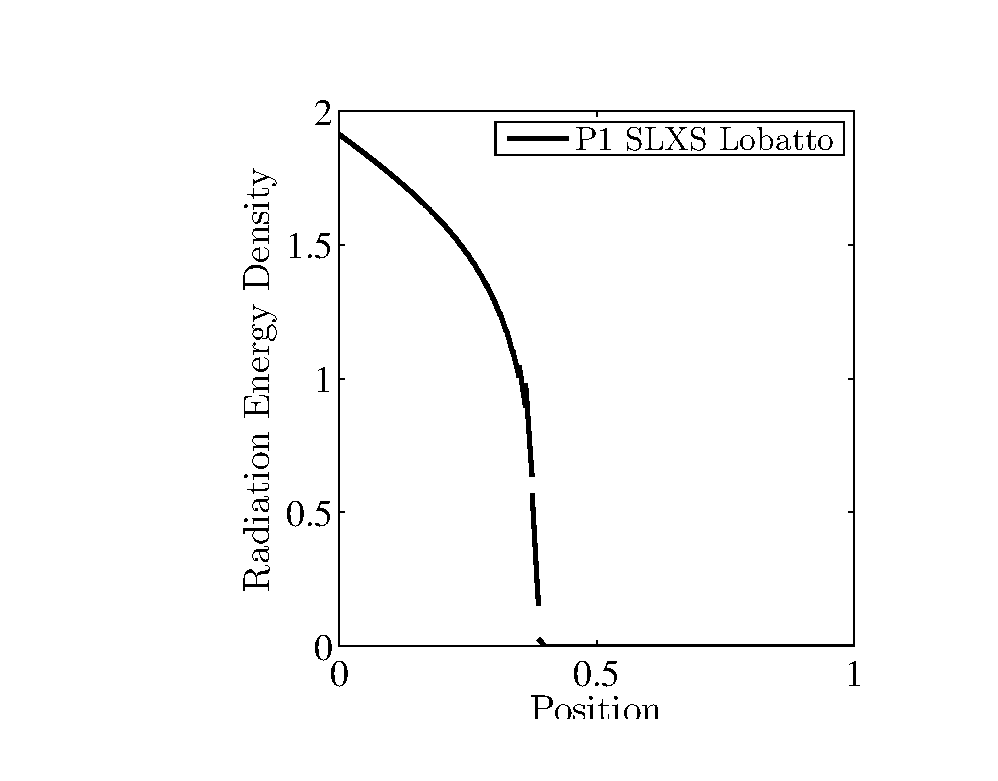
\includegraphics[width=9.5cm,trim=1.2in  0.2in 0.75in 0.5in,clip=true]{chapter6_grey_radtran/Dissertation_Data/SLXS_Lobatto_80_Cells_Radiation.pdf}
\caption{Linear SLXS Lobatto angle integrated intensity solution with 80 cells.}
\label{fig:linear_slxs_full_rad}
\end{figure}
%
%
\begin{figure}[!htp]
\centering
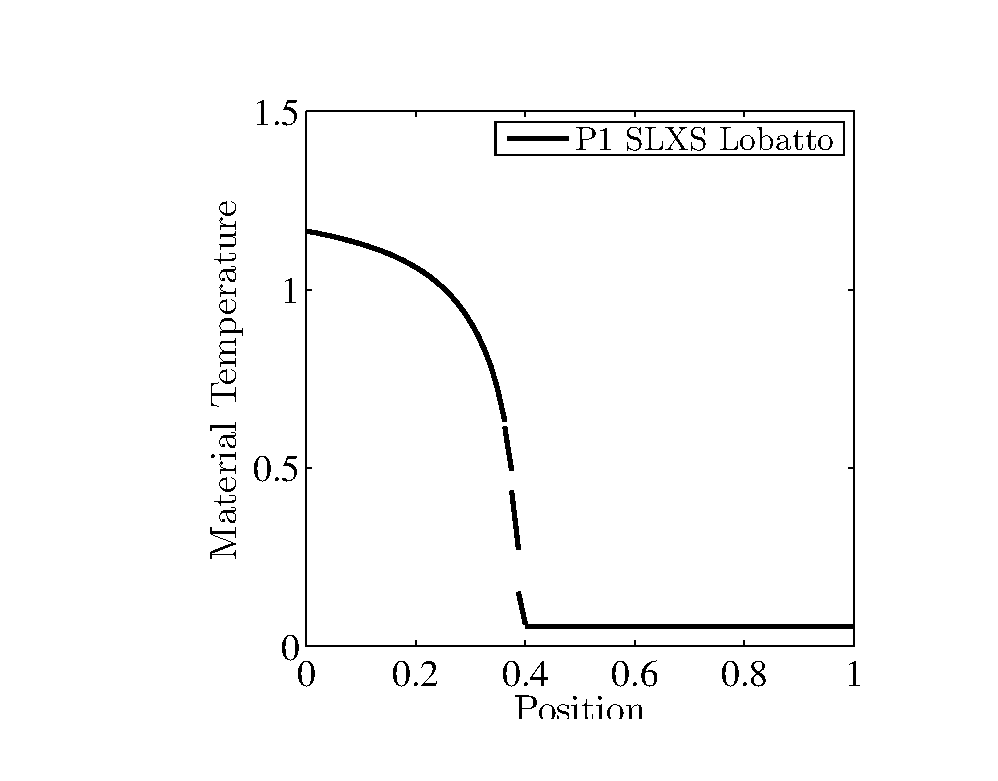
\includegraphics[width=9.5cm,trim=1.2in  0.2in 0.75in 0.5in,clip=true]{chapter6_grey_radtran/Dissertation_Data/SLXS_Lobatto_80_Cells_Temperature.pdf}
\caption{Linear SLXS Lobatto temperature solution with 80 cells.}
\label{fig:linear_slxs_full_temp}
\end{figure}
%

We now consider the effects of spatial mesh refinement on the unity Marshak wave problem.  
We first consider the linear SLXS Lobatto scheme, looking at a zoom in near the wavefront of the radiation profile in \fig{fig:lobatto_convergence_rad} and the material temperature profile in \fig{fig:lobatto_convergence_temp}
\begin{figure}[!hbp]
\centering
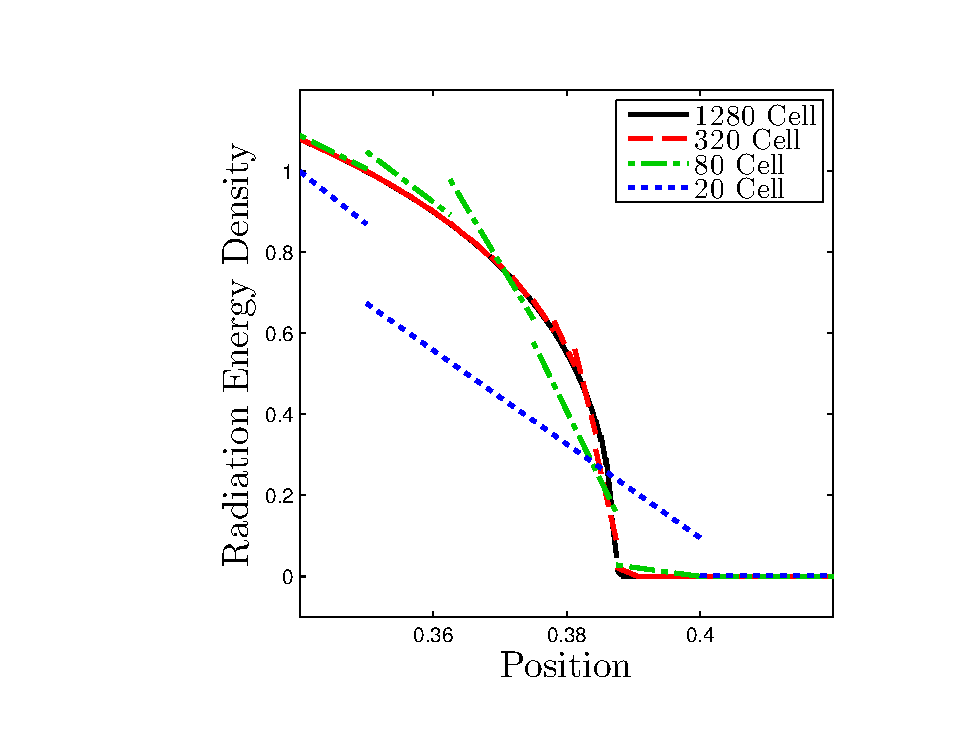
\includegraphics[width=10cm,trim=1.0in  0.2in 0.5in 0.5in,clip=true]{chapter6_grey_radtran/Dissertation_Data/Reorder_Marshak_Zoom_Radiation_SL_Lobatto_P1_Cell_Refinement.pdf}
\caption{Linear SLXS Lobatto radiation solution near wavefront with increasing spatial mesh refinement.}
\label{fig:lobatto_convergence_rad}
\end{figure}
%
%
\begin{figure}[!htp]
\centering
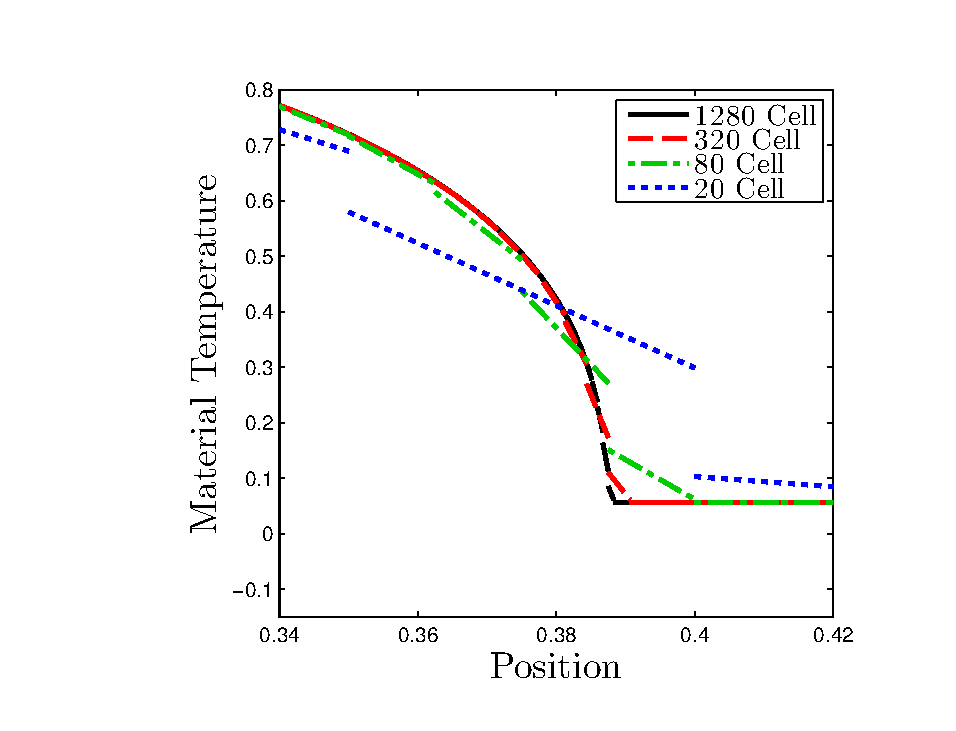
\includegraphics[width=10cm,trim=1.0in  0.2in 0.5in 0.5in,clip=true]{chapter6_grey_radtran/Dissertation_Data/Reorder_Marshak_Zoom_Temperature_SL_Lobatto_P1_Cell_Refinement.pdf}
\caption{Linear SLXS Lobatto temperature solution near wavefront with increasing spatial mesh refinement.}
\label{fig:lobatto_convergence_temp}
\end{figure}
Though the changes are subtle, we can see that mesh refinement actually changes the location of both the radiation and temperature profile wavefront, with the changes more prominent in the material temperature profile, \fig{fig:lobatto_convergence_temp}.
The changes in the material temperature profile are more pronounced than in the radiation profile because linear SLXS Lobatto more accurately calculates the radiation intensity than the material temperature, converging $E_{\phi} \propto 2$ and $E_T \propto 1$.
Equivalent plots to \fig{fig:lobatto_convergence_rad} and \fig{fig:lobatto_convergence_temp} are provided in \fig{fig:gauss_convergence_rad} and \fig{fig:gauss_convergence_temp}, respectively for the quartic SLXS Gauss scheme.
\begin{figure}[!hbp]
\centering
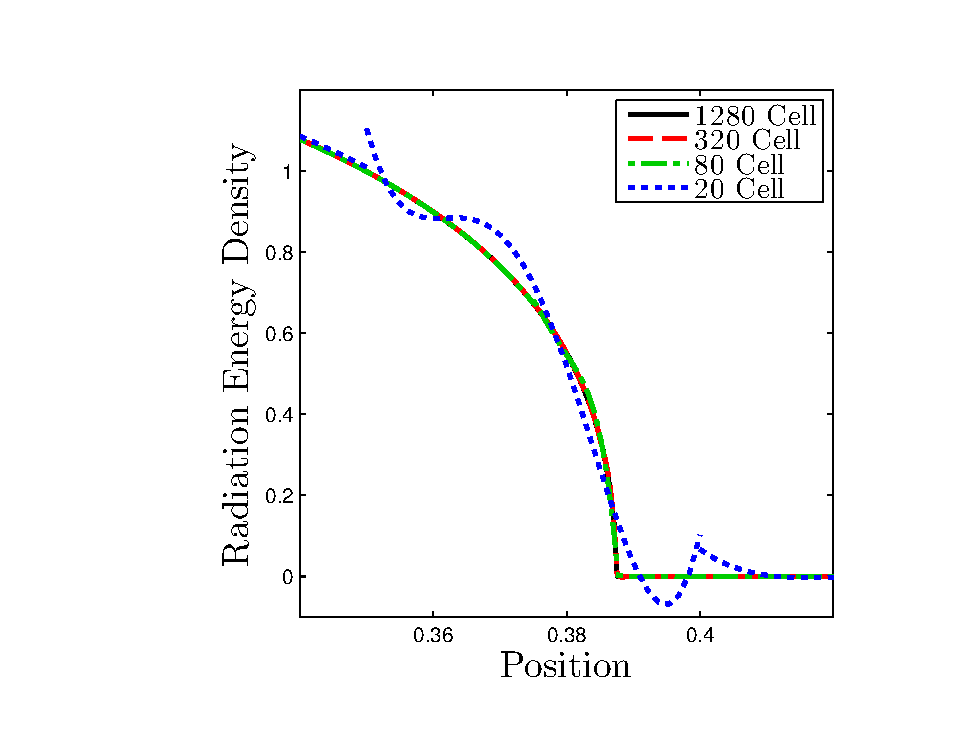
\includegraphics[width=10cm,trim=1.0in  0.2in 0.5in 0.5in,clip=true]{chapter6_grey_radtran/Dissertation_Data/Reorder_Marshak_Zoom_Radiation_SL_Gauss_P4_Cell_Refinement.pdf}
\caption{Quartic SLXS Gauss radiation solution near wavefront with increasing spatial mesh refinement.}
\label{fig:gauss_convergence_rad}
\end{figure}
%
%
\begin{figure}[!htp]
\centering
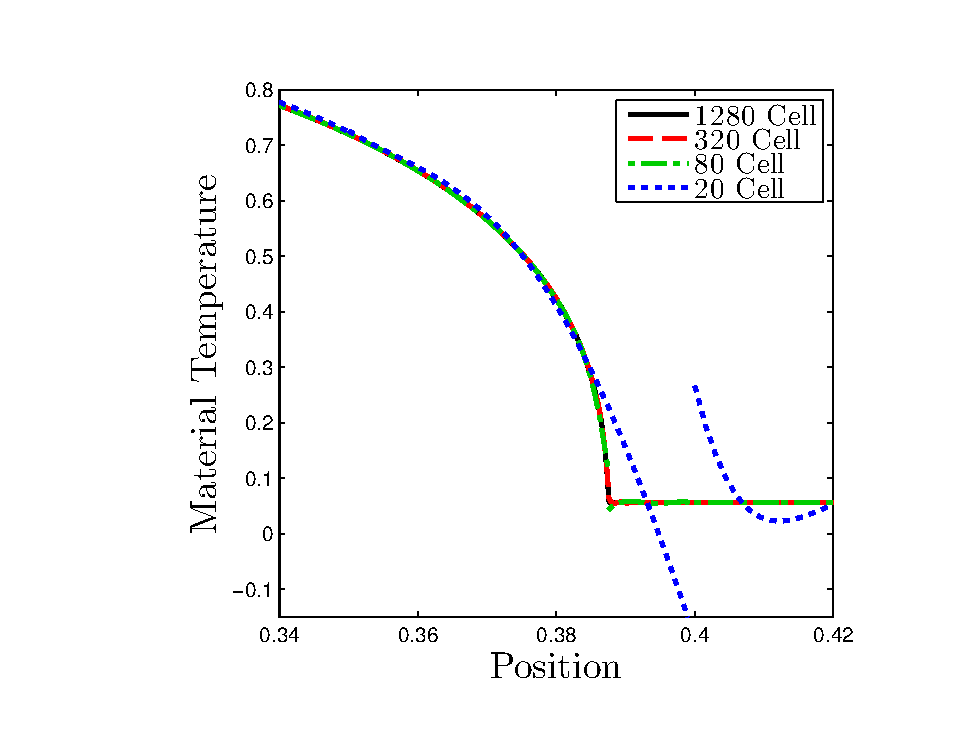
\includegraphics[width=10cm,trim=1.0in  0.2in 0.5in 0.5in,clip=true]{chapter6_grey_radtran/Dissertation_Data/Reorder_Marshak_Zoom_Temperature_SL_Gauss_P4_Cell_Refinement.pdf}
\caption{Quartic SLXS Gauss temperature solution near wavefront with increasing spatial mesh refinement.}
\label{fig:gauss_convergence_temp}
\end{figure}
Due to the SLXS Gauss' high order of spatial convergence, few changes are noticeable with mesh refinement, except when moving from 20 to 80 cells.
However, when moving from 20 to 80 cells, the Gibbs' phenomena near the solution discontinuity are no longer visible, except for a very small negativity in the temperature solution.
All solutions for this spatial mesh refinement study use $\Delta t = 1.5625 \times 10^{-4}$.

We now examine the effect of increasing DFEM trial space degree, on a fixed mesh of 320 spatial cells using SLXS Lobatto, focusing on the region near the Marshak wavefront.
In \fig{fig:p_convergence_rad} we plot the angle integrated intensity profile and plot the temperature profile in \fig{fig:p_convergence_temp}
\begin{figure}[!htp]
\centering
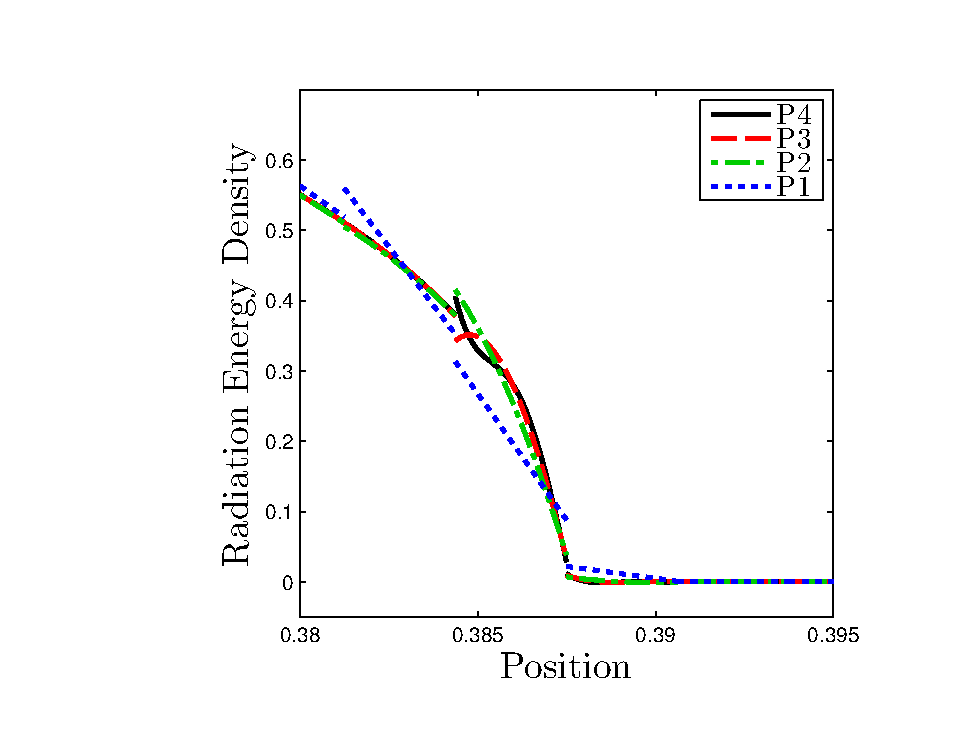
\includegraphics[width=10cm,trim=1.0in  0.2in 0.5in 0.5in,clip=true]{chapter6_grey_radtran/Dissertation_Data/Pointless_Marshak_Zoom_Radiation_Lobatto_P_Refinement.pdf}
\caption{SLXS Lobatto radiation energy density solution with 320 cells for different $P$ near Marshak wavefront.}
\label{fig:p_convergence_rad}
\end{figure}
%
\begin{figure}[!hbp]
\centering
\includegraphics[width=10cm,trim=1.0in  0.2in 0.5in 0.5in,clip=true]{chapter6_grey_radtran/Dissertation_Data/Pointless_Marshak_Zoom_Temperature_Lobatto_P_Refinement.pdf}
\caption{SLXS Lobatto material temperature solution with 320 cells for different $P$ near Marshak wavefront.}
\label{fig:p_convergence_temp}
\end{figure}
Increasing $P$ make the wavefront in the radiation profile sharper, but at a resolution of 320 cells, none of the $P$ considered result in a visually continuous solution.
The most notable changes with increase $P$ come in the temperature profile, where linear SLXS Lobatto does not form a sharp interface, whereas all of the higher $P$ schemes capture the non-smooth transition more accurately.

Before looking at very high spatial resolution solutions, we first consider the effect of time step refinement on the unity Marshak wave problem in \fig{fig:time_refinement_rad} for the angle integrated intensity and in \fig{fig:time_refinement_temp} for the material temperature solution.
Both \fig{fig:time_refinement_rad} and \fig{fig:time_refinement_temp} use a quartic SLXS Gauss spatial discretization with 1280 cells.
The effects of decreasing time step size are non-trivial near the wavefront.
As seen in \fig{fig:time_refinement_rad}, at lower time resolutions, $\Delta t$ and $\frac{\Delta t}{4}$, the wavefront is visibly not uniform concave down, with several ``wiggles'' in the radiation profile in the heated region of the slab.
Additionally, increased temporal resolution causes the discontinuity at the leading edge of the wavefront to sharpen.
In \fig{fig:time_refinement_temp}, the effects of increased time resolution are the same as in \fig{fig:time_refinement_rad}.
However, increased time resolution more noticeably sharpens the discontinuity in the temperature profile than it eliminates wavefront wiggles, though in \fig{fig:time_refinement_temp} the $\Delta t$ curve is not strictly concave down in the heated region of the slab near the wavefront.
%
%
\begin{figure}[!htp]
\centering
\includegraphics[width=10cm,trim=1.0in  0.2in 0.5in 0.5in,clip=true]{chapter6_grey_radtran/Dissertation_Data/Time_Refinement_Zoom_Radiation.pdf}
\caption{Quartic SLXS Lobatto radiation energy density solution with 1280 cells for different time refinements near the Marshak wavefront.}
\label{fig:time_refinement_rad}
\end{figure}
%
%
\begin{figure}[!hbp]
\centering
\includegraphics[width=10cm,trim=1.0in  0.2in 0.5in 0.5in,clip=true]{chapter6_grey_radtran/Dissertation_Data/Time_Refinement_Zoom_Temperature.pdf}
\caption{Quartic SLXS Lobatto temperature solution with 1280 cells for different time refinements near the Marshak wavefront.}
\label{fig:time_refinement_temp}
\end{figure}

\pagebreak

We now discuss highly resolved $S_2$ solutions to the Marshak wave problem.
Our hope is that with sufficient spatial resolution and higher order DFEM, we are able to resolve transport boundary layers.
Our highest resolution simulation uses ten thousand spatial mesh cells.
Given the initial, cold temperature of the slab is roughly $T=0.056$,  $\sigma_t = \sigma_a = \frac{1}{T^3}$, then the total slab optical thickness is roughly 5700 MFP thick, and when using ten though cells, each mesh cell is roughly $0.57$ MFP thick.  
As noted by Larsen, Morel, and Miller \cite{thick_diffusion_larsen}, this type of mesh spacing is neither optically thick nor thin.
To answer whether ten thousand mesh cells is sufficient, we first consider \fig{fig:res_zoom_comparison} where we compare the results of cubic SLXS Lobatto schemes that use
\begin{enumerate}
\item ten thousand spatial cells, with ten thousand time steps and the SDIRK 3-3 scheme,
\item ten thousand spatial cells, with one thousand time steps and the SDIRK 3-3 scheme, and 
\item 1280 spatial cells, with six thousand time steps of the SDIRK 3-3 scheme.
\end{enumerate} 
\begin{figure}[!htp]
\centering
\includegraphics[width=13cm,trim=1.0in  0.75in 1.0in 1.0in,clip=true]{chapter6_grey_radtran/Dissertation_Data/Zoom_10k_Phi.pdf}
\caption{Plot of the radiation energy density on a logarithmic scale for different high resolution simulations near the Marshak wavefront.}
\label{fig:res_zoom_comparison}
\end{figure}
Missing' segments in \fig{fig:res_zoom_comparison} are caused by negative angle integrated intensity solutions.
The 1280 cell simulation has only 1 negative node.
The ten thousand cell simulation that uses one thousand time steps has a total of 8 negative nodes; one entire cell has a negative radiation energy density, and two other cells have at least one node with a negative radiation energy density.
Since the ten thousand cell simulation with ten thousand time steps does not have any negative radiation energy densities, it is clear then that accurate TRT simulations require both space and time refinement.

In \fig{fig:boundary_layer}, we plot the angular intensities for $\mu=\pm\frac{1}{\sqrt{3}}$ of the ten thousand cell, ten thousand time step simulation.  
\begin{figure}[!htp]
\centering
\includegraphics[width=11cm,trim=0.5in  0.0in 0.5in 0.5in,clip=true]{chapter6_grey_radtran/Dissertation_Data/50_Cells_at_Wavefront_Intensity_Log.pdf}
\caption{Plot of the angular intensity on a logarithmic scale near the transport boundary layer at the Marshak wave front.}
\label{fig:boundary_layer}
\end{figure}
Clearly the radiation traveling from the hot to cold region, $I_d(\mu_d=\frac{1}{\sqrt{3}},x)$ has a large boundary layer near the thermal, but the rapid rise in angular intensity appears to be smooth, suggesting we have resolved the radiation boundary layer. 
Unfortunately, to obtain high resolution everywhere at all times in the simulation requires a uniform spatial mesh, and using ten thousand total cells leaves only ten cells available to resolve the transport boundary layer present at $x\in[0.387 0.388]$ at $t=1.0$.

We conclude our discussion of the unity Marshak wave problem by considering higher $S_N$ solutions to the Marshak wave problem.  
First, we compare the $S_8$ solution to the $S_2$ solution for material temperature in \fig{fig:s2_vs_s8_temperature} and for radiation energy density in \fig{fig:s2_vs_s8_radiation}.  
The $S_8$ solution in \figs{fig:s2_vs_s8_temperature}{fig:s2_vs_s8_radiation} was generated using quartic SLXS Gauss with five thousand spatial cells, the SDIRK 2-2 scheme, and approximately ten thousand time steps.  
The $S_2$ solution is the same solution as plotted in \fig{fig:boundary_layer}.
\begin{figure}[!htp]
\centering
\includegraphics[width=11cm,trim=1.0in  0.5in 0.2in 0.6in,clip=true]{chapter6_grey_radtran/S8_vs_S2_Material_Temperature.pdf}
\caption{$S_8$ and $S_2$ material temperature profiles.}
\label{fig:s2_vs_s8_temperature}
\end{figure}
%
\begin{figure}[!htp]
\centering
\includegraphics[width=11cm,trim=1.0in  0.3in 0.2in 0.5in,clip=true]{chapter6_grey_radtran/S8_vs_S2_Radiation_Energy_Density.pdf}
\caption{$S_8$ and $S_2$ radiation energy density profiles.}
\label{fig:s2_vs_s8_radiation}
\end{figure}
The $S_8$ solution exhibits many of the qualitative features we would expect a transport solution to exhibit. % versus the $S_2$ solution which is very close to the diffusion solution.
For example, we expect the transport solution to have a higher temperature solution near the problem boundary, with a more rapid drop in both the material temperature and radiation energy density/angle integrated intensity solutions relative to a diffusion solution.
Additionally, we expect the transport material temperature and radiation energy density solution to penetrate farther into the slab than the diffusion solution, but with a less steep gradient.
Figures \ref{fig:s2_vs_s8_radiation}-\ref{fig:s2_vs_s8_temperature} both exhibit these behaviors, caused by the transport solution becoming more and more like $\delta(\mu-1)$ in optically thick regions. 
However, we did not expect the non-smooth features near $x=0.2$.
We suspect the kinks in the temperature and radiation energy density profiles is caused by the transition of the most glancing $\mu_d >0$ from being dominated by boundary contributions to being dominated by photon re-emission.
To verify this, we plot the $S_8$ intensity solution in \fig{fig:s8_intensity_full}.
\begin{figure}[!htp]
\centering
\includegraphics[width=16cm,trim=1.5in  0.5in 0.2in 1in,clip=true]{chapter6_grey_radtran/S8_Intensity_SemiLogy.pdf}
\caption{Log plot of $S_8$ intensities for the unity Marshak wave problem.}
\label{fig:s8_intensity_full}
\end{figure}

We now zoom in to the boundary layer intensities near $x=0.2$ and near the thermal wave front.
In \fig{fig:s8_zoom_glance}, it is clear that the intensity in the direction of $\mu=+0.1834$ experiences a rapid variation as the incident flux from the boundary is attenuated, and the isotropic emission from the heated regions of the slabs becomes the main contributor to $I(\mu_d = +0.1834)$.
It is also clear that despite having 25 cells with quartic DFEM in the region $x\in[.18,.185]$, the factor $\approx 7\times$ step drop in $I(\mu_d = +0.1834)$ cannot be fully resolved. 
\begin{figure}[!ht]
\centering
\includegraphics[width=12cm,trim=0.5in  0.2in 0.5in 0.5in,clip=true]{chapter6_grey_radtran/Dissertation_Data/S8_pos_mu_glance_boundary_layer_log.pdf}
\caption{Logarithmic plot of intensity near glancing $\mu=+0.1834$ boundary layer. }
\label{fig:s8_zoom_glance}
\end{figure}The more glancing $\mu_d$, the sooner the transition, relative to the left boundary.


Near the hot/cold material interface, all angular intensities experience a boundary layer transition.  
Using higher order DFEM and high spatial resolution, it appears that we are able to resolve these boundary layers, given the smooth profile of angular intensity for every direction in the quadrature set.
\begin{figure}[!ht]
\centering
\includegraphics[width=16cm,trim=1.5in  0.2in 0.5in 0.75in,clip=true]{chapter6_grey_radtran/Dissertation_Data/S8_thermal_wavefront_boundary_layer.pdf}
\caption{Logarithmic plot of intensity boundary layers near thermal wavefront.}
\label{fig:s8_zoom_thermal_wavefront}
\end{figure}

Next we investigate the structure of an $S_{32}$ solution with 1000 spatial cells, quartic SLXS Gauss, and five thousand time steps using the SDIRK 2-2 time integration scheme.
The material temperature solution is plotted in \fig{fig:s8_vs_s32_temperature} against the $S_8$ solution that uses quartic SLXS Gauss,  five thousand spatial cells, and ten thousand SDIRK time integration steps.
Likewise, the angle integrated intensity solutions are compared in \fig{fig:s8_vs_s32_radiation}.
\begin{figure}[!htp]
\centering
\includegraphics[width=16cm,trim=1.5in  0.2in 0.5in 0.75in,clip=true]{chapter6_grey_radtran/Dissertation_Data/S8_vs_S32_Material_Temperature.pdf}
\caption{Comparison of $S_8$ and $S_{32}$ material temperature profiles for the unity Marshak wave problem.}
\label{fig:s8_vs_s32_temperature}
\end{figure}
%
%
\begin{figure}[!htp]
\centering
\includegraphics[width=16cm,trim=1.5in  0.2in 0.5in 0.75in,clip=true]{chapter6_grey_radtran/Dissertation_Data/S8_vs_S32_Radiation.pdf}
\caption{Comparison of $S_8$ and $S_{32}$ angle integrated intensity solutions for the unity Marshak wave problem.}
\label{fig:s8_vs_s32_radiation}
\end{figure}
Even with $S_{32}$ Gauss quadrature, we continue to see non-smooth dips in both the material temperature and angle integrated intensity profiles, however the dips are significantly smaller for the $S_{32}$ solution as compared to the $S_8$ solution, particularly for the material temperature profile.
In \fig{fig:s8_vs_s32_radiation}, the $S_{32}$ exhibits four smaller dips as compared to the single, larger dip associated with $S_8$.
Suspecting these are caused by glancing incidence angles in the quadrature set, we plot the angular intensity for all $\mu_d > 0$ in \fig{fig:s32_intensity}.
\begin{figure}[!htp]
\centering
\includegraphics[width=16cm,trim=1.5in  0.2in 0.5in 0.75in,clip=true]{chapter6_grey_radtran/Dissertation_Data/S32_Intensity.pdf}
\caption{$S_{32}$ intensity solutions for all $\mu_d > 0$, for the unity Marshak wave problem.}
\label{fig:s32_intensity}
\end{figure}
As with the $S_8$ solution, the dips in $\phi$ are associated with corresponding dips in $I_d$ for glancing $\mu_d>0$.\
The discontinuity associated with $\mu_d = 0.3319$ is obscured in \fig{fig:s8_vs_s32_radiation} as the dip occurs just as the $S_{32}$ angle integrated intensity cross over the $S_8$ angle integrated intensity solution.
The $\mu_d=0.0483$ intensity jump in \fig{fig:s32_intensity} causes the greatest effect in \fig{fig:s8_vs_s32_radiation} for two reasons.  
First, the most glancing quadrature angle is attenuated the most rapidly and as such would be expected to have the greatest drop in value.
Second, Gauss angular quadrature assigns the greatest weight to the quadrature points most near $\mu_d = 0$. 
Surprisingly, the $S_8$ and $S_{32}$ calculations have nearly identical positions and values of the temperature and angle integrated intensity solution near the problem boundary and the hot/cold interface.  
If however, the goal is a smooth transport solution, the value of $N$ required to create a smooth $S_N$ $\phi$ solution appears to be much higher than $S_{32}$, due to the presence of time ray effects \cite{lewis_book}.

The kinks observed in the higher order $S_N$ solutions for the Marshak wave problem are examples of time ray effects.
Typically these are not observed in thermal radiative transfer simulations, because as the material heats up, the magnitude of photon re-emission sources quickly becomes comparable to and surpasses the rapidly attenuated incident photon contribution to the angular intensity.
If the observed kinks are time ray effects, they will be worse at earlier times and less pronounced at later times, due to the attenuation of the incident intensity contribution over a greater distance (as the wave front advances) and photon re-emission from the increased material temperature.
To verify that the observed kinks are indeed time ray effects, consider \fig{fig:phi_time_slices} and \fig{fig:temp_time_slices} which show the $S_{32}$ Marshak wave radiation energy density and material temperature at different points in time, computed using 1000 spatial cells, cubic SLXS Lobatto, $\Delta t_{max} = 2 \times 10^{-4}$, and the SDIRK 2-2 time scheme.
\begin{figure}[!htp]
\centering
\includegraphics[width=17cm,trim=2in  0.5in 0.5in 0.75in,clip=true]{chapter6_grey_radtran/Dissertation_Data/S32_Time_Ray_Effects_Radiation_Cv1_SigA1.pdf}
\caption{$S_{32}$ radiation energy density at different times for the unity Marshak wave problem.}
\label{fig:phi_time_slices}
\end{figure}
\begin{figure}[!hbp]
\centering
\includegraphics[width=17cm,trim=2in  0.4in 0.5in 0.75in,clip=true]{chapter6_grey_radtran/Dissertation_Data/S32_Time_Ray_Effects_Temperature_Cv1_SigA1.pdf}
\caption{$S_{32}$ material temperature solution at different times for the unity Marshak wave problem.}
\label{fig:temp_time_slices}
\end{figure}
While the earliest time material temperature solution does not have visually large kinks due to ray effects, ray effects can be seen in the radiation energy density solution at all times considered.
To observe that the radiation energy density ray effects decrease in magnitude at later times, first consider the radiation energy density at $t=0.1$, given in \fig{fig:t01_radiation_energy}, and then compare to the radiation energy density at $t=2.0$ given in \fig{fig:t2_radiation_energy}.  
Figure \ref{fig:t01_radiation_energy} and \fig{fig:t2_radiation_energy} use the same $y$-axis scaling.  
Comparing \figs{fig:t01_radiation_energy}{fig:t2_radiation_energy}, it is clear that the radiation energy drops associated with ray effects are significantly larger at $t=0.1$ than at $t=2.0$.
\begin{figure}[!htp]
\centering
\includegraphics[width=16cm,trim=2in  0.5in 0.5in 0.75in,clip=true]{chapter6_grey_radtran/Dissertation_Data/S32_T01_Radiation_Equal_Height.pdf}
\caption{$S_{32}$ radiation energy density at $t=0.1$ for the unity Marshak wave problem.}
\label{fig:t01_radiation_energy}
\end{figure}
\begin{figure}[!hbp]
\centering
\includegraphics[width=16cm,trim=2in  0.4in 0.5in 0.75in,clip=true]{chapter6_grey_radtran/Dissertation_Data/S32_T2_Radiation.pdf}
\caption{$S_{32}$ radiation energy density at $t=2$ for the unity Marshak wave problem.}
\label{fig:t2_radiation_energy}
\end{figure}
The $\mu$ labels in \figs{fig:t01_radiation_energy}{fig:t2_radiation_energy} correspond to the directional cosines of angular intensities that experience a significant drop at those locations.
 as shown in \fig{fig:t01_intensity} and \fig{fig:t2_intensity} for $t=0.1$ and $t=2$, respectively.
\begin{figure}[!htp]
\centering
\includegraphics[width=16cm,trim=2in  0.5in 0.5in 0.75in,clip=true]{chapter6_grey_radtran/Dissertation_Data/S32_T01_Intensity.pdf}
\caption{$S_{32}$ angular intensity for $\mu_d>0$ at $t=0.1$ for the unity Marshak wave problem.}
\label{fig:t01_intensity}
\end{figure}
\begin{figure}[!hbp]
\centering
\includegraphics[width=16cm,trim=2in  0.4in 0.5in 0.75in,clip=true]{chapter6_grey_radtran/Dissertation_Data/S32_T2_Intensity.pdf}
\caption{$S_{32}$ angular intensity for $\mu_d>0$ at $t=2$ for the unity Marshak wave problem.}
\label{fig:t2_intensity}
\end{figure}
Comparing \fig{fig:t01_intensity} to \fig{fig:t2_intensity} clearly shows that as time progresses, ray effects decrease, in \fig{fig:t01_intensity}, there are six angular intensities that have a discontinuous jump from being dominated by incident boundary conditions and heated material photon re-emission whereas in \fig{fig:t2_intensity}, at most 4 directions experience a non-smooth transition from being dominated by incident boundary contributions ti being dominated by photon re-emission.

Though ray effects are inherent to discrete ordinates calculations, the severe time ray effects observed in the unity Marshak wave problem are more a function of problem parameters than of a fundamental flaw with discrete ordinates methods applied to thermal radiative transfer.
The choice to define $a=c=C_v=1$ and $\sigma_t = \sigma_a = \frac{1}{T^3}$ was chosen by previous authors, and did not correspond to a physical scaling of typical physical material properties.
This can easily be seen by considering an alternative simulation, where we define $\sigma_t = \sigma_a = \frac{1000}{T^3}$.
Under this assumption, even the heated material is optically thick, and photon re-emission quickly becomes the more dominant contributor to angular intensity than incident photon energy.
In \fig{fig:sig_a_1000_radiation}, radiation energy density solutions for the modified unity Marshak wave problem at different times are given for a simulation using 1000 spatial cells, $x\in[0,1]$, linear SLXS Lobatto, and SDRIK 2-2 time differencing.
\begin{figure}[!htp]
\centering
\includegraphics[width=8cm,trim=1in  0.5in 1in 0.75in,clip=true]{chapter6_grey_radtran/Dissertation_Data/More_Times_P1_S8_Time_Ray_Effects_Radiation_Cv1_SigA1000.pdf}
\caption{$S_{8}$ radiation energy density solutions for the modified unity Marshak wave problem with $\sigma_a = \frac{1000}{T^3}$ at different times.}
\label{fig:sig_a_1000_radiation}
\end{figure}
\begin{figure}[!hbp]
\centering
\includegraphics[width=8cm,trim=1in  0.6in 1.0in 0.75in,clip=true]{chapter6_grey_radtran/Dissertation_Data/More_Times_P1_S8_Time_Ray_Effects_Temperature_Cv1_SigA1000.pdf}
\caption{$S_{8}$ material temperature solutions for modified unity Marshak wave problem with $\sigma_a = \frac{1000}{T^3}$ at different times.}
\label{fig:sig_a_1000_temperature}
\end{figure}
Figures \ref{fig:sig_a_1000_radiation}-\ref{fig:sig_a_1000_temperature} make it clear that changing $\sigma_a$ fundamentally alters the ``unity'' Marshak wave problem.
The thermal wave does not penetrate nearly as far in the modified unity Marshak wave problem, but also does not exhibit any time ray effects as compared to the original unity Marshak wave problem.

\subsection{Physical Marshak Wave Problem}

We now consider a Marshak wave problem that uses a physical units that has been considered repeatedly in the literature \cite{negative_trt,time_adaptive_diffusion,physical_marshak}.
The problem consists of a $0.05~[cm]$ slab at an initial temperature of $1~[eV]$, heated from the left with an isotropic $1~[keV]$ photon source.
After $0.1~[sh]$, $1~[sh]=10^{-8}~[sec]$, the thermal wave will have nearly passed through the entire domain.
The material heat capacity is temperature independent, $C_v = 0.3~[\frac{jerks}{cm^3~keV}]$, $\sigma_a = \frac{300}{T^3} [cm^{-1}]$, with $T$ in keV, and $\sigma_s = 0$.
Representative angle integrated intensity and temperature solutions at various times are given in \fig{fig:physical_slices_radiation} and \fig{fig:physical_slices_temperature}.    
The representative solutions are generated using 100 spatial cells with cubic SLXS Lobatto and $S_8$ Gauss angular quadrature.
\begin{figure}[!htp]
\centering
\includegraphics[width=16cm,trim=2in  0.4in 0.5in 0.75in,clip=true]{chapter6_grey_radtran/Dissertation_Data/100C_Physical_Marshak_Wave_Radiation_Times.pdf}
\caption{$S_{8}$ angle integrated intensity solutions at various times for physical Marshak wave problem.}
\label{fig:physical_slices_radiation}
\end{figure}
\begin{figure}[!hbp]
\centering
\includegraphics[width=16cm,trim=2in  0.4in 0.5in 0.75in,clip=true]{chapter6_grey_radtran/Dissertation_Data/100C_Physical_Marshak_Wave_Temperature_Times.pdf}
\caption{Temperature solutions at various times for physical Marshak wave problem.}
\label{fig:physical_slices_temperature}
\end{figure}
We note that \fig{fig:physical_slices_radiation} does not exhibit any time ray effects.  
This problem description, given in the cm-sh-keV unit system, has a heat capacity on the same order as $C_v=1$ in the unity Marshak wave problem.  
In addition the product of the radiation constant, $a = 0.01372~[\frac{jerks}{cm^3~keV^4}]$, and speed of light, $c=299.792~[cm/sh]$, $ac = 4.113~\left[\frac{jerks}{cm^2~sh~keV^4}\right]$, is on the same order as $a=c=1$ from the unity Marshak wave problem.
The only thing that is significantly different in this problem is that the numerator in the definition of $\sigma_a$ is a factor of 300 larger in this physical Marshak wave problem than the unity Marshak wave problem, reaffirming that the time ray effects observed in the unity Marshak wave problem are atypical of discrete ordinate solutions applied to the thermal radiative transfer equations, and a function more of the optically thin nature of the unity Marshak wave problem at higher temperatures.

Our main interest in the physical Marshak wave problem is to test our different adaptive time criteria.  
Using the notation of \eqt{eq:adaptive_change}, in all of the results that follow, we will assume $\Delta T_{goal} = 0.01$, unless otherwise stated.
We first apply  each adaptive method to a linear SLXS discretization of the physical Marshak wave using 100 spatial cells.
Time step size selected as function of the simulated time in the simulation is given for each method in \fig{fig:linear_time_steps} with $\Delta t_{goal} =0.01$.
\begin{figure}[!htp]
\centering
\includegraphics[width=17cm,trim=2in  0.4in 0.5in 0.75in,clip=true]{chapter6_grey_radtran/Dissertation_Data/P1_vs_time.pdf}
\caption{Time step sizes selected for different adaptive criterion applied to a linear SLXS Lobatto discretization of the physical Marshak wave problem.}
\label{fig:linear_time_steps}
\end{figure}
For this particular problem, the point-wise adaptive criterion taken from \cite{time_adaptive_diffusion}, yields the same time step selection at every time step as the modified point-wise criterion with $T_{offset}=0~eV$ because no negative temperature solutions are generated with a linear SLXS Lobatto discretization of this problem.
The 4-5 single time steps of the point-wise criterion time step size trace that are orders of magnitude smaller than neighboring time step sizes are artifacts of outputting the solution at selected times, and taking the required time step to output exactly at those times.
The volumetric scheme with $N_{cg}$ chooses larger time step sizes than the point-wise adaptive criterion as expected, since a $1\%$ change average over a volume permits a much larger increase in $T$ than a $1\%$ increase maximum at any one point.
We also note the large number of sharps peaks and valleys present in all traces of time step size in \fig{fig:linear_time_steps}.  
Each valley, or time step minimum comes as the thermal wave crosses into the next mesh cell.
Additionally, we note that since the speed of the thermal front slows as time progresses, the peaks occur at a greater frequency for earlier times than near the end of the simulation.
The slowing of the wave can be more clearly visualized by viewing \fig{fig:physical_slices_temperature},.
At $t=0.01 ~[sh]$, the wave is at approximately $x=0.0125~[cm]$.
If the thermal wave propagated at a constant speed, then at $t=0.08~[sh]$, we would expect the thermal wave to be near $x= .1~[cm]$.  
However, the thermal wave is only located at approximately $x<0.04~[cm]$ in \fig{fig:physical_slices_temperature}.
The number of time steps each adaptive method took, as well as the number of time steps that were rejected are given in \tbl{tbl:p1_steps}. 
Rejected time steps are those $\Delta t^n$, that after computing $\Delta T$ using $\widetilde{T}^{n+1}$ and $\widetilde{T}^n$, $\Delta T > 1.2 \Delta T_{goal}$, thus indicating $\Delta t^n$ was too large, requiring a repeat of the time step from $t^n$ to $t^{n+1}$.
\begin{table}[!htp]
\centering
\caption{Time steps taken for different adaptive time stepping criterion for physical Marshak wave problem discretized with linear SLXS Lobatto and 100 cells.}
\label{tbl:p1_steps}
\begin{tabular}{|c|c|c|}
\hline
{} &  Total Steps & Rejected Steps \\
\hline
Point-wise & 77648 & 0 \\
\hline
Modified Point-wise, &    &  \\
$T_{offset} = 0~[eV]$ &  77648  &  0\\
\hline
Volumetric, $N_{cg} = 1$ & 49957   & 0\\
\hline
\end{tabular}
\end{table}

We now examine the performance of each adaptive time criterion applied to a cubic SLXS Lobatto discretization of the physical Marshak wave problem using 100 spatial cells.
As seen in \fig{fig:physical_slices_temperature}, negative temperature solutions are present at the thermal wavefront.
The negative temperature solutions are cause the simplest point-wise adaptive criterion, \eqt{eq:pointwise_adaptive}, to fail.
For all attempted spatial resolutions, the point-wise adaptive criterion always attempts to take vanishingly small time steps.
To show that the challenging nature of an under resolved Marshak wave problem causes the point-wise adaptive criterion to fail, and that adaptive time step selection techniques 
are  compatible with higher order DFEM schemes for TRT simulations, we consider an alternative to the Marshak wave problem.
Using the same spatial domain, temporal domain, and material properties as the physical Marshsak wave problem, but the slab is heated with  a distributed volumetric radiation source equivalent to a black body material radiating energy at a temperature of 1~keV instead of an incident 1~keV temperature source.
Thus, 
\begin{enumerate}
\item the solution is constant in space, 
\item opacities do not vary spatially,
\item the radiation solution is strictly non-negative, 
\item negative temperatures are not generated, and
\item the point-wise adaptive criterion does not fail.
\end{enumerate}
A trace of $\Delta t$ selected at each time step, normalized by dividing the time step number $n$ by the total number of time steps, $n_{final}$, required by a given adaptive criterion to complete the problem is given in \fig{fig:source_trace} for a simulation of the source driven problem using cubic SLXS Lobatto and 1000 spatial cells.
Figure \ref{fig:source_trace} shows that for a spatially constant solution all three adaptive criteria yield the same time step size, as might be expected.  However, this is still sufficient to demonstrate that adaptive time step selection criteria may be used for higher order DFEM TRT simulations, but they must be designed in a sufficiently sophisticated way that adaptive technique can survive the numerical shortcomings of low spatial resolution problems.
\begin{figure}[!htp]
\centering
\includegraphics[width=16cm,trim=2in  0.4in 0.5in 0.75in,clip=true]{chapter6_grey_radtran/Dissertation_Data/Source_dt_trace.pdf}
\caption{Time step sizes selected for adaptive criteria for volumetric radiation source driven problem.}
\label{fig:source_trace}
\end{figure}

Table \ref{tbl:p3_counts} summarizes the number of time steps required to complete the physical Marshak wave problem for the modified point-wise and volumetric adaptivity criterion using 100 equally spaced cells and the cubic SLXS Lobatto scheme.
\begin{table}[!htp]
\centering
\caption{Time steps taken for different adaptive time stepping criterion for physical Marshak wave problem discretized with cubic SLXS Lobatto and 100 cells.}
\label{tbl:p3_counts}
\begin{tabular}{|c|c|c|}
\hline
{} &  Total Steps & Rejected Steps \\
\hline
Modified Point-wise, &   Failed & \\
$T_{offset} = 0~[eV]$ &    &   \\
\hline
Modified Point-wise, &   558495  & 3 \\
$T_{offset} = 1~[eV]$ &     &  \\
\hline
Modified Point-wise, &  397608  & 2\\
$T_{offset} = 5~[eV]$ &    &  \\
\hline
Modified Point-wise, &  184033  & 0\\
$T_{offset} = 50~[eV]$ &    &  \\
\hline
Volumetric, $N_{cg} = 1$ &  1320259  & 976 \\
\hline
Volumetric, $N_{cg} = 2$ & 68182   & 1252 \\
\hline
Volumetric, $N_{cg} = 5$ & 29607   & 1346 \\
\hline
Volumetric, $N_{cg} = 10$ & 16657   & 1449 \\
\hline
Volumetric, $N_{cg} = 25$ & 9716   & 1631 \\
\hline
Volumetric, $N_{cg} = 50$ & 7124   & 1736 \\
\hline
Volumetric, $N_{cg} = 100$ & 5936   & 1808 \\
\hline
\end{tabular}
\end{table}
Comparing the number of steps taken in \tbl{tbl:p3_counts} to \tbl{tbl:p1_steps} makes it clear that higher order DFEM methods applied to TRT simulations challenge the performance of simple time adaptive criteria.
Indeed, the modified point-wise scheme struggles, requiring $T_{floor}$ to be artificially high to yield reasonable time step sizes.
Interestingly though, using an artificially high $T_{floor}$ did not yield significantly larger maximum time step sizes.  
As seen in \fig{fig:mod_comparison}, the largest time step size chosen with the modified point-wise adaptive scheme is the same regardless whether $T_{offset} = 1~[ev]$ or $T_{offset} = 50~[eV]$.
\begin{figure}[!htp]
\centering
\includegraphics[width=16cm,trim=2in  0.4in 0.5in 0.75in,clip=true]{chapter6_grey_radtran/Dissertation_Data/Modified_Pointwise_T_offset.pdf}
\caption{Time step sizes for modified point-wise adaptive criteria for cubic SLXS Lobatto discretization of the physical Marshak wave problem with different $T_{offset}$.}
\label{fig:mod_comparison}
\end{figure}

Though the volumetric adaptive criterion with $N_{cg}=1$  requires more than twice as many time steps to solve the same Marshak wave problem with cubic rather than linear DFEM, the modified point-wise scheme requires more than $7\times$ time steps to solve the same problem with higher DFEM order. 
Additionally, the modified point-wise adaptive criterion is not universally applicable without a large $T_{offset}$, as evidenced by the failure the modified point-wise adaptive criterion for $T_{offset}=0~[eV]$, and exceedingly high number of time steps required with $T_{offset}=1~[eV]$.
Consider now the trace of $\Delta t$ selection as a function of time in the simulation in \fig{fig:50ev_1C} for the modified point-wise scheme with $T_{offset}=50~[eV]$ to the volumetric adaptive criterion with $N_{cg}=1$.
\begin{figure}[!htp]
\centering
\includegraphics[width=16cm,trim=2in  0.4in 0.5in 0.75in,clip=true]{chapter6_grey_radtran/Dissertation_Data/Volumetric_1C_vs_50ev_in_time.pdf}
\caption{Time step sizes for volumetric and modified point-wise adaptive criteria for cubic SLXS Lobatto discretization of the physical Marshak wave problem.}
\label{fig:50ev_1C}
\end{figure}
We see all of the same features we observed for the linear SLXS Lobatto solution: peak/valley pairs as the thermal wave enters each successive cell in the mesh and the volumetric scheme taking larger time steps than the point-wise scheme.  
However, it is important to note that though the volumetric scheme takes larger time steps, it also adapts and takes much smaller time steps when necessary, smaller even than the modified point-wise adaptive scheme with $T_{offset}=50~[eV]$.

Table \ref{tbl:p3_counts} demonstrates that larger values of $N_{cg}$ take significantly larger average time steps, but how does $\Delta t$ selection vary for different $N_{cg}$ as a function of time?
In \fig{fig:1c_vs_100c}, the two extrema of $N_{cg}$ for this particular spatial discretization, there appear to be no significant differences between the trend in time of the different values of $N_{cg}$, with the exception that for $N_{cg}=100$, $\Delta t$ is chosen approximately $10\times-100\times$ larger than $\Delta t$ for $N_{cg}=1$.  
Both $N_{cg}=1$ and $N_{cg}=100$ have the peaks and valleys associated with the thermal wave passing into each new mesh cell.
\begin{figure}[!htp]
\centering
\includegraphics[width=16cm,trim=2in  0.4in 0.5in 0.75in,clip=true]{chapter6_grey_radtran/Dissertation_Data/Volumetric_Trace_1cg_vs_100cg_vs_time.pdf}
\caption{Time step sizes for volumetric adaptive criteria with $N_{cg}=1$ and $N_{cg}=100$ for }
\label{fig:1c_vs_100c}
\end{figure}
This is not the case for intermediate values of $N_{cg}$.  
Consider \fig{fig:5c_vs_25c} that plots $\Delta t$ selected during the simulation for the volumetric adaptive criterion using $N_{cg}=5$ and $N_{cg}=25$.
\begin{figure}[!htp]
\centering
\includegraphics[width=16cm,trim=2in  0.4in 0.5in 0.75in,clip=true]{chapter6_grey_radtran/Dissertation_Data/Volumetric_Trace_5cg_vs_25cg_vs_time.pdf}
\caption{Time step sizes for volumetric adaptive criteria with $N_{cg}=1$ and $N_{cg}=100$. }
\label{fig:5c_vs_25c}
\end{figure}
The dips we have thus far seen and associated with the thermal wave crossing individual mesh cells are present, but so are other, lower frequency dips.
These slower, periodic drops in $\Delta t$ are associated with the thermal wave crossing from one volumetric adaptive grouping into another.  
If a problem was run until the slab was at a uniform temperature, i.e. the thermal wave has passed entirely through the slab, there would be $N_{groups}-1$ repetitive groupings.

Finally, we wish to examine whether the vastly different values of time steps taken by the different adaptive criteria.
As no analytic solution exists, we must simply compare the results of simulations that use different adaptive criteria at some time value.
Assuming that any temporal introduced by taking too large of a time step accumulates, we look at the angle integrated intensity and temperature solutions at $t=0.1~[sh]$.
Further, assuming that the largest differences occur between the simulation that took the most time steps and the simulation that took the fewest time steps, in \figs{fig:time_difference_radiation}{fig:time_difference_temperature} we compare the angle integrated intensity and temperature solutions of simulations, respectively, of the modified point-wise adaptive criterion with $T_{offset} = 1~[eV]$, and the volumetric adaptive criterion with $N_{cg}=100$.
\begin{figure}[!htp]
\centering
\includegraphics[width=16cm,trim=2in  0.4in 0.5in 0.75in,clip=true]{chapter6_grey_radtran/Dissertation_Data/100C_Physical_Marshak_Wave_Radiation_Adaptive_Comparison_Final_1eV.pdf}
\caption{Comparison of angle integrated intensity for different adaptive criteria at $t=0.1~[sh]$.}
\label{fig:time_difference_radiation}
\end{figure}
\begin{figure}[!htp]
\centering
\includegraphics[width=16cm,trim=2in  0.4in 0.5in 0.75in,clip=true]{chapter6_grey_radtran/Dissertation_Data/100C_Physical_Marshak_Wave_Temperature_Adaptive_Comparison_Final_1eV.pdf}
\caption{Comparison of temperature for different adaptive criteria at $t=0.1~[sh]$.}
\label{fig:time_difference_temperature}
\end{figure}
Despite the modified point-wise scheme with $T_{offset}=1~[eV]$ using nearly $95\times$ more time steps than the volumetric criterion with $N_{cg}=100$, with this level of spatial accuracy, there is no appreciable visual difference between the two solutions, suggesting that the volumetric adaptive criteria is more efficient than the modified point-wise criteria when applied to higher order DFEM TRT simulations.

\newpage

\section{Effectiveness of MIP DSA for TRT Iterative Acceleration}
\label{sec:mip_results}

As of yet, we have failed to discuss the iterative performance of the modified interior penalty diffusion synthetic operator (MIP DSA) applied to the grey thermal radiative transfer equations.
Though the problems we have considered are not necessarily optically thick, we have used MIP DSA to iteratively solve all problems.
A large number of the problems we have considered are not optically thick, in part because we were interested in spatial error convergence.
In \tbl{tbl:iteration_count}, we give a sampling of the average number of iterations required to update the intensity for a given thermal iteration for the problems we have considered thus far.

Several observations can be made regarding the data in \tbl{tbl:iteration_count}.  
Most importantly, MIP DSA applied to the grey TRT is a stable iterative scheme and at worst requires as many iterations as source iteration alone.
Also, the number of iterations for MIP DSA and SI are nearly equal only for most of the problems we have considered, but for those where SI requires larger number of iterations, the ratio of SI+DSA iterations to SI alone iterations grows.
Finally, MIP DSA is compatible with the self-lumping DFEM schemes we have developed that explicitly account for the within cell variation of opacity and heat capacity.

\begin{table}[!htp]
\centering
\caption{Iteration count for different TRT model problems.}
\begin{tabular}{|c|c|c|c|}
\hline
Problem Description & Scheme & Average DSA+SI & Average SI \\
{}									&				 &  Iterations & Iterations  \\
\hline
MMS Constant Time & Linear  & 1.4 & 2.4 \\
4 cells 					& SLXS Lobatto & {} & {} \\
\hline
MMS Constant Time	 & Cubic 			 & 1.6 & 2.3 \\
8 cells 						& SLXS Lobatto & {} & {} \\
\hline
MMS Constant Time	 & Cubic 				 & 1.8 & 1.8 \\
128 cells 					& SLXS Lobatto & {} & {} \\
\hline
MMS1 						& Quadratic 		& 2.0 & 13.5 \\
2 cells 				& SLXS Gauss 		& {}  & {} \\
\hline
MMS1 						& Quadratic 	& 3.0 & 13.6 \\
32 cells 				& SLXS Gauss 	& {} & {} \\
\hline
MMS1	 				& Quadratic  & 4.0 & 13.5 \\
128 cells 		& SLXS Gauss & {} & {} \\
\hline
MMS1 					& Quadratic		& 4.2 & 13.5 \\
256 cells 		& SLXS Gauss 	& {} & {} \\
\hline
MMS2 						& Linear	 & 1.0 & 2.7 \\
2 cells 					& SLXS Gauss & {} & {} \\
\hline
MMS Constant Space 									& Quartic 				 & 17.0 & 39.0 \\
Alexander 3-3, $\Delta t=1$					& SLXS Lobatto 			& {}  & {} \\
\hline
MMS Constant Space 										& Quartic 				 & 6.6 & 11.7 \\
Alexander 3-3, $\Delta t=\frac{1}{8}$	& SLXS Lobatto 			& {}  & {} \\
\hline
MMS Constant Space 										& Quartic 				 & 2.3 & 4.9 \\
Alexander 3-3, $\Delta t=\frac{1}{128}$	& SLXS Lobatto 			& {}  & {} \\
\hline
Marshak Wave 									&  Linear			 & 2.1 & 2.9 \\
20 cells, largest $\Delta t$	& SLXS Lobatto & {} 		 & {} \\
\hline
\end{tabular}
\label{tbl:iteration_count}
\end{table}

To demonstrate the iterative effectiveness of MIP DSA we now present a problem designed solely to be optically thick.
We again define a dimensionless problem, $a=c=1$.
We assume a constant $C_v = 0.05$, define $x\in[0,100]$, $t\in[0,5]$, $\sigma_s = 0$, and $\sigma_a = \frac{5000}{T^2}$.
Initially, the slab is in thermodynamic equilibrium at a temperature of $T=0.5$, and is heated with an incident current of $100$ on the left hand side of the slab.
We difference the problem with linear SLXS Lobatto using 50 spatial cells, implicit Euler in time differencing, and a maximum time step size of $\Delta t_{max} = 0.1$.
The average number of transport iterations per thermal iteration is given in \tbl{tbl:high_iter_count}.
\begin{table}[!ht]
\centering
\caption{Iteration count for a very optically thick TRT problem.}
\label{tbl:high_iter_count}
\begin{tabular}{|c|c|}
\hline
Intensity  						& Average Intensity					\\				
Iterative Strategy		& Iterations Per Thermal Iteration \\
\hline
DSA		&   10  \\ 
\hline
SI  &   18378 \\
\hline
\end{tabular}
\end{table}
Clearly, MIP DSA can significantly reduce the iterative work required to solve the grey TRT equations, but the majority of problems we have considered are not very optically thick.

In optically thick and diffusive problems such as this, the traditional convergence condition of 
\benum
\norm{ \phi^{(\ell+1) } - \phi^{(\ell)} } < \epsilon_{\phi} \pec
\eenum
can lead to false convergence \cite{adams_larsen_fast_iterative}.
Noting that our chosen point-wise convergence condition $\text{change\_phi} < \epsilon_{\phi}$, with $\text{change\_phi}$ as defined in \eqt{eq:change_phi}  is not a true mathematical norm, we would still like to investigate the issue of false convergence.
To do so, we first define a norm based convergence condition:
\benum
\norm{ \phi^{(\ell+1)} - \phi^{(\ell)} }_{L^1} < \epsilon_{\phi} \norm{ \phi^{(\ell+1)}}_{L^1} \pep
\label{eq:l1}
\eenum
In \eqt{eq:l1}, we have multiplied the right hand side by $\norm{ \phi^{(\ell+1)} }$ to allow for a uniform convergence criteria, regardless of the physical scale of any particular problem.
As shown in \cite{adams_larsen_fast_iterative}, we may eliminate false convergence by normalizing our convergence condition with $1-\rho$,
\benum
\frac{\norm{\phi^{(\ell+1)} - \phi^{(\ell)}_{L^1} } }{ 1- \rho}< \epsilon_{\phi} \pec
\label{eq:rho_convergence}
\eenum
where $\rho$ is the spectral radius, which we estimate as:
\benum
\rho \approx \frac{ \norm{\phi^{(\ell+1)} - \phi^{(\ell)} } }{ \norm{\phi^{(\ell)} - \phi^{(\ell-1)} } }\pep
\eenum
In \tbl{tbl:rho_iters}, we plot the average number of iterations required to converge $\phi$ for each time step for our optically thick and diffusive test problem.  For all methods, we used $\epsilon_{\phi} = 10^{-10}$.
\begin{table}[!hbp]
\centering
\caption{Average number of inner iterations per thermal iteration using different convergence criteria.}
\label{tbl:rho_iters}
\begin{tabular}{|c|c|c|c|}
\hline
{}  &  $\text{change\_phi} <\epsilon_{\phi}$ & 
		$ \frac{\norm{ \phi^{(\ell+1)} - \phi^{(\ell)} }_{L^1} }{ \norm{ \phi^{(\ell+1)}}_{L^1}  } < \epsilon_{\phi}$  & 
		$\frac{\norm{\phi^{(\ell+1)} - \phi^{(\ell)}_{L^1} } }{ (1- \rho) \norm{\phi^{(\ell+1)}} }< \epsilon_{\phi} $\\
		\hline
SI & 18378 & 6382 & 22563 \\
\hline
DSA & 10 & 7 & 7 \\
\hline
\end{tabular}
\end{table}
Table \ref{tbl:rho_iters} clearly indicates that for optically thick, diffusive problems, the near unity spectral radius can lead to false iterative convergence, and as such should be accounted for explicitly via \eqt{eq:rho_convergence}.  
We also remark that our choice of using $\norm{\phi^{(\ell+1)} }_{L^1}$ as a physical scaling constant could possibly be improved upon, as $\norm{\phi^{(\ell+1)}}_{L^1}$ is dominated by the already heated region, whereas the greatest changes in $\phi$ are occurring near the thermal wavefront.



